\clearpage

\section{Event Simulation and Selection \label{sec:simulation}}

\subsection{Sample generation}

We study the performance of the super-razor variables in the context of searches for new physics appearing in two different scenarios:
\begin{itemize}
\item Pair production of sleptons (selectrons $\tilde{e}^\pm$ or smuons $\tilde{\mu}^\pm$) decaying to electrons or muons, respectively, and neutralinos ($\tilde{\chi}_1^0$) with 100\% branching ratio (BR) for both left- or right-handed sparticles.
\item Pair production of the lightest chargino ($\tilde{\chi}_1^\pm$) decaying into $\tilde{\chi}_1^0$ and a $W$-boson with 100\% BR. We require both $W$-bosons to decay leptonically while accounting for the SM $W$-boson branching ratio.
\end{itemize}
Event samples corresponding to these signal models were generated using {\tt MadGraph5} \cite{Alwall:2011uj} and {\tt Pythia 6.4} \cite{Sjostrand:2006za}, with up to two extra matched jets. 
We consider slepton and chargino masses between the LEP bound ($\sim 100$~GeV) up to 450~GeV, with neutralino masses varying between zero and 20 GeV less than their respective parent sparticle masses. Production cross sections for these signal events were obtained for the LHC with $\sqrt{s} = 8$~TeV at next-to-leading order (NLO) using {\tt Prospino} \cite{Beenakker:1999xh}. All superpartners except for the neutralino and active slepton flavor/chargino were decoupled by setting their mass to 2.5~TeV and the chargino was assumed to be wino-like. In the mass intervals considered, the resulting cross sections range from $\sim 100 - 1$~fb for both flavors of sleptons and $\sim 5000-100$~fb for the chargino, with the cross-sections as a function of sparticle mass illustrated in Figure~\ref{fig:sigma}. 
\begin{figure}[ht]
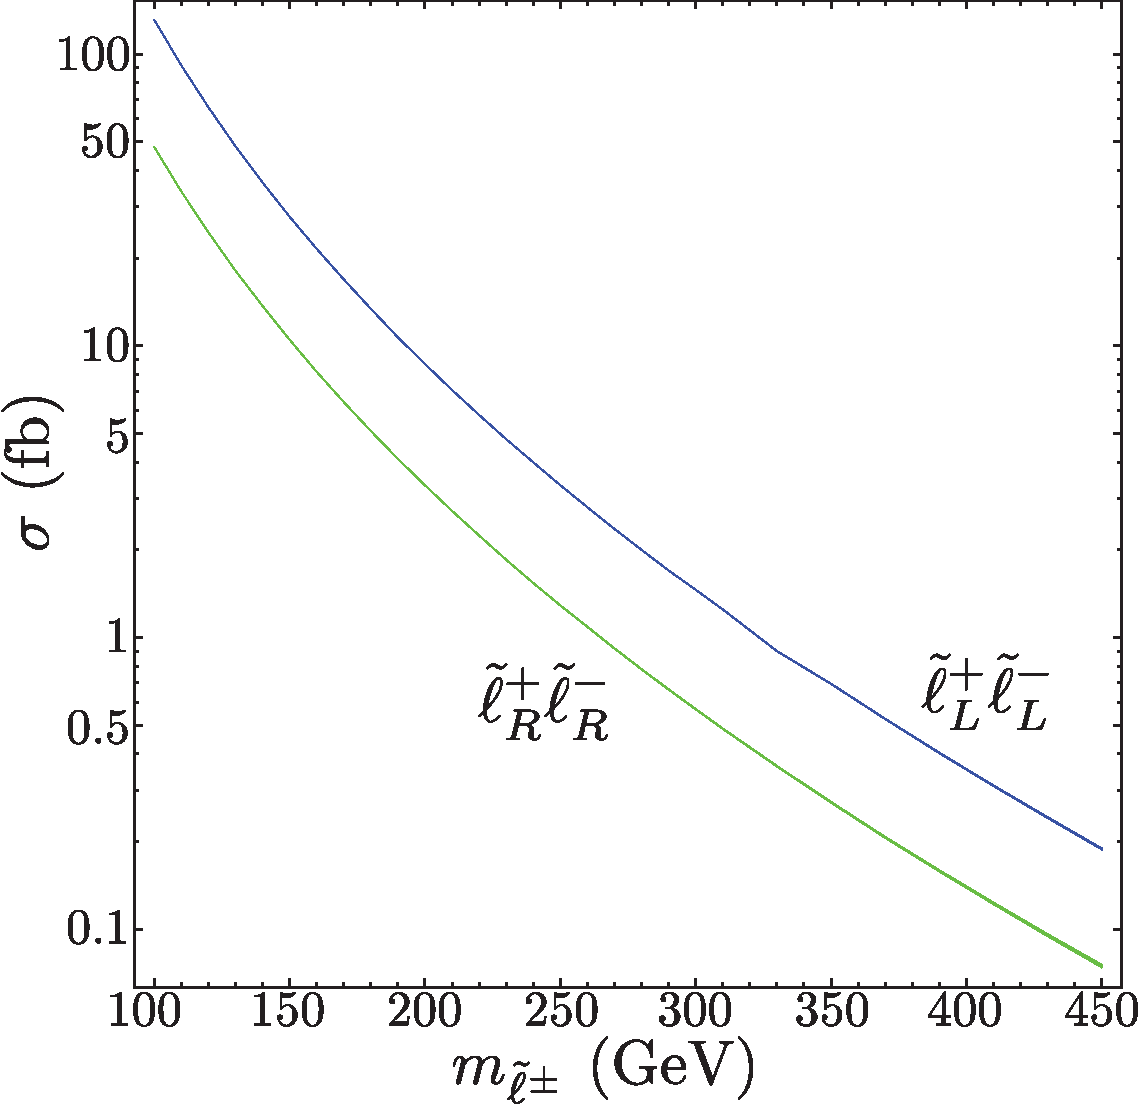
\includegraphics[width=0.29\columnwidth]{fig/sectionIII/sleptonxs2.pdf}\hspace{5em}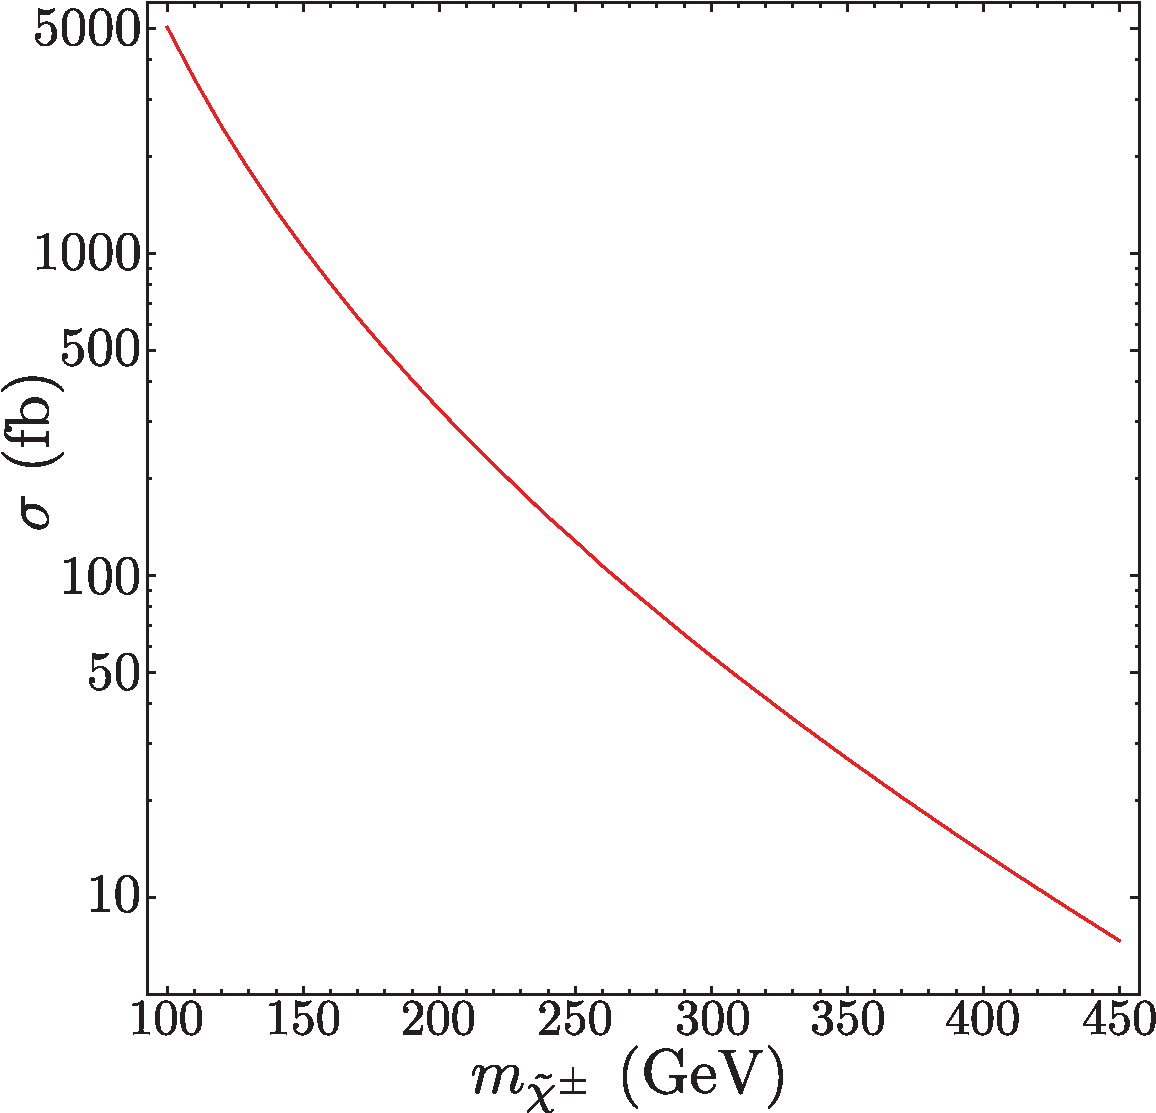
\includegraphics[width=0.3\columnwidth]{fig/sectionIII/charginoxs2.pdf} 
\caption{Left: $1^{\rm st}$ or $2^{\rm nd}$ generation left-handed (blue) and right-handed (green) slepton pair production cross sections. Right: Chargino pair production cross section. Cross sections calculated using {\tt Prospino} \cite{Beenakker:1999xh} at NLO for the LHC with $\sqrt{s}=8$~TeV. Theoretical errors indicated by width of lines. \label{fig:sigma}}
\end{figure}

In order to estimate the sensitivity of the CMS and ATLAS experiments to these putative signals we also generate event samples corresponding to the primary SM backgrounds in the di-lepton final state: di-boson ($W^+W^-$, $W^\pm Z$, and $ZZ$) production, Drell-Yan $(Z/\gamma^*\to\ell\ell)+$jets, and top pair production. Event samples were generated for all channels in {\tt MadGraph5}+{\tt Pythia 6.4},
with up to two extra matched jets and cross-sections calculated from the same generator configuration. 

\subsection{Detector simulation and baseline selection~\label{sec:baseline}}

All of the event samples, for both signal and background processes, are analyzed using the PGS toy detector simulation, from which reconstructed leptons (electrons and muons) are identified and jets are clustered. For all the kinematic distributions and results presented in this work, simulated events are included only if they satisfy baseline selection requirements. 

Each event is required to have exactly two reconstructed leptons with $p_{T} > 20$~GeV and $|\eta| < 2.5$. Events are discarded which have more than two leptons satisfying this requirement. Furthermore, these leptons are required to have opposite charge. The combination of these requirements reduces the yields of selected events corresponding to di-boson backgrounds such as $WZ$ and $ZZ$ where there are either more than two leptons reconstructed or the two leptons arise from the decays of different bosons. Events are assigned to one of three flavor categories corresponding to same flavor (SF) where there are either two reconstructed electrons ($e^-e^+$) or muons ($\mu^-\mu^+$) and opposite flavor (OF), containing
$e\mu$ events. An additional requirement of $m(\ell\ell) > 15$~GeV is applied to events falling in the SF categories in order to reject backgrounds with low-mass di-lepton resonances.

Jets are clustered from simulated calorimeter cells using FastJet \cite{Cacciari:2011ma} and the anti-$k(t)$ algorithm \cite{Cacciari:2008gp}.
Events containing at least one jet with $p_{T} > 25$~GeV and $|\eta| < 2.5$ which is identified as $b$-tagged are discarded from the event sample in order to reduce the contribution from events containing top quarks. The number of reconstructed jets is used to classify events into one of three jet multiplicity categories: 0 jet, $1$ jet and $\ge 2$ jet. This jet counting scheme is based on jets with with $p_{T} > 30$~GeV and $|\eta| < 3$. Furthermore, events are discarded if either of the two reconstructed leptons falls within a cone of $\Delta R \equiv \sqrt{\Delta\eta^{2}+\Delta\phi^2} = 0.4$ around any of the reconstructed jets in the event. Unless otherwise indicated, kinematic distributions include the sum of all three flavor and jet multiplicity categories. 

\subsection{Comparison of different kinematic variables}

We evaluate the potential for the variable $M_{\Delta}^{R}$ to be used in a search for di-slepton and di-chargino production signals by comparing it with similar variables used in CMS and ATLAS searches. The CMS search for slepton production in the di-lepton final state~\cite{CMS-PAS-SUS-13-006} utilizes the variable $M_{CT\perp}$ \cite{Matchev:2009ad,Tovey:2008ui} while the analogous ATLAS analysis \cite{ATLAS-CONF-2013-049} includes requirements on the variable $M_{T2}$~\cite{Lester:1999tx,Barr:2003rg} in definitions of signal regions sensitive to the presence of di-leptons following from slepton decays. The distributions of each of these kinematic variables, $M_{\Delta}^{R}$, $M_{CT\perp}$, and $M_{T2}$, are shown in Figure~\ref{fig:compare} for slepton and chargino signals with various sparticle mass combinations.

The behavior of each of the three variables is similar. Each is sensitive to the quantity $M_{\Delta}$ for signal events, with a sharp edge or endpoint at the true value. The shape of each distribution is largely insensitive to the absolute value of $M_{\Delta}$, such that distributions are nearly identical when scaled by $M_{\Delta}$ (differences are observed when the parent sparticle and the neutralino approach degeneracy). The similarities between these $M_{\Delta}$ sensitive variables are indicative of the fact that they are highly correlated and represent largely redundant information about events. 

\begin{figure}[ht]
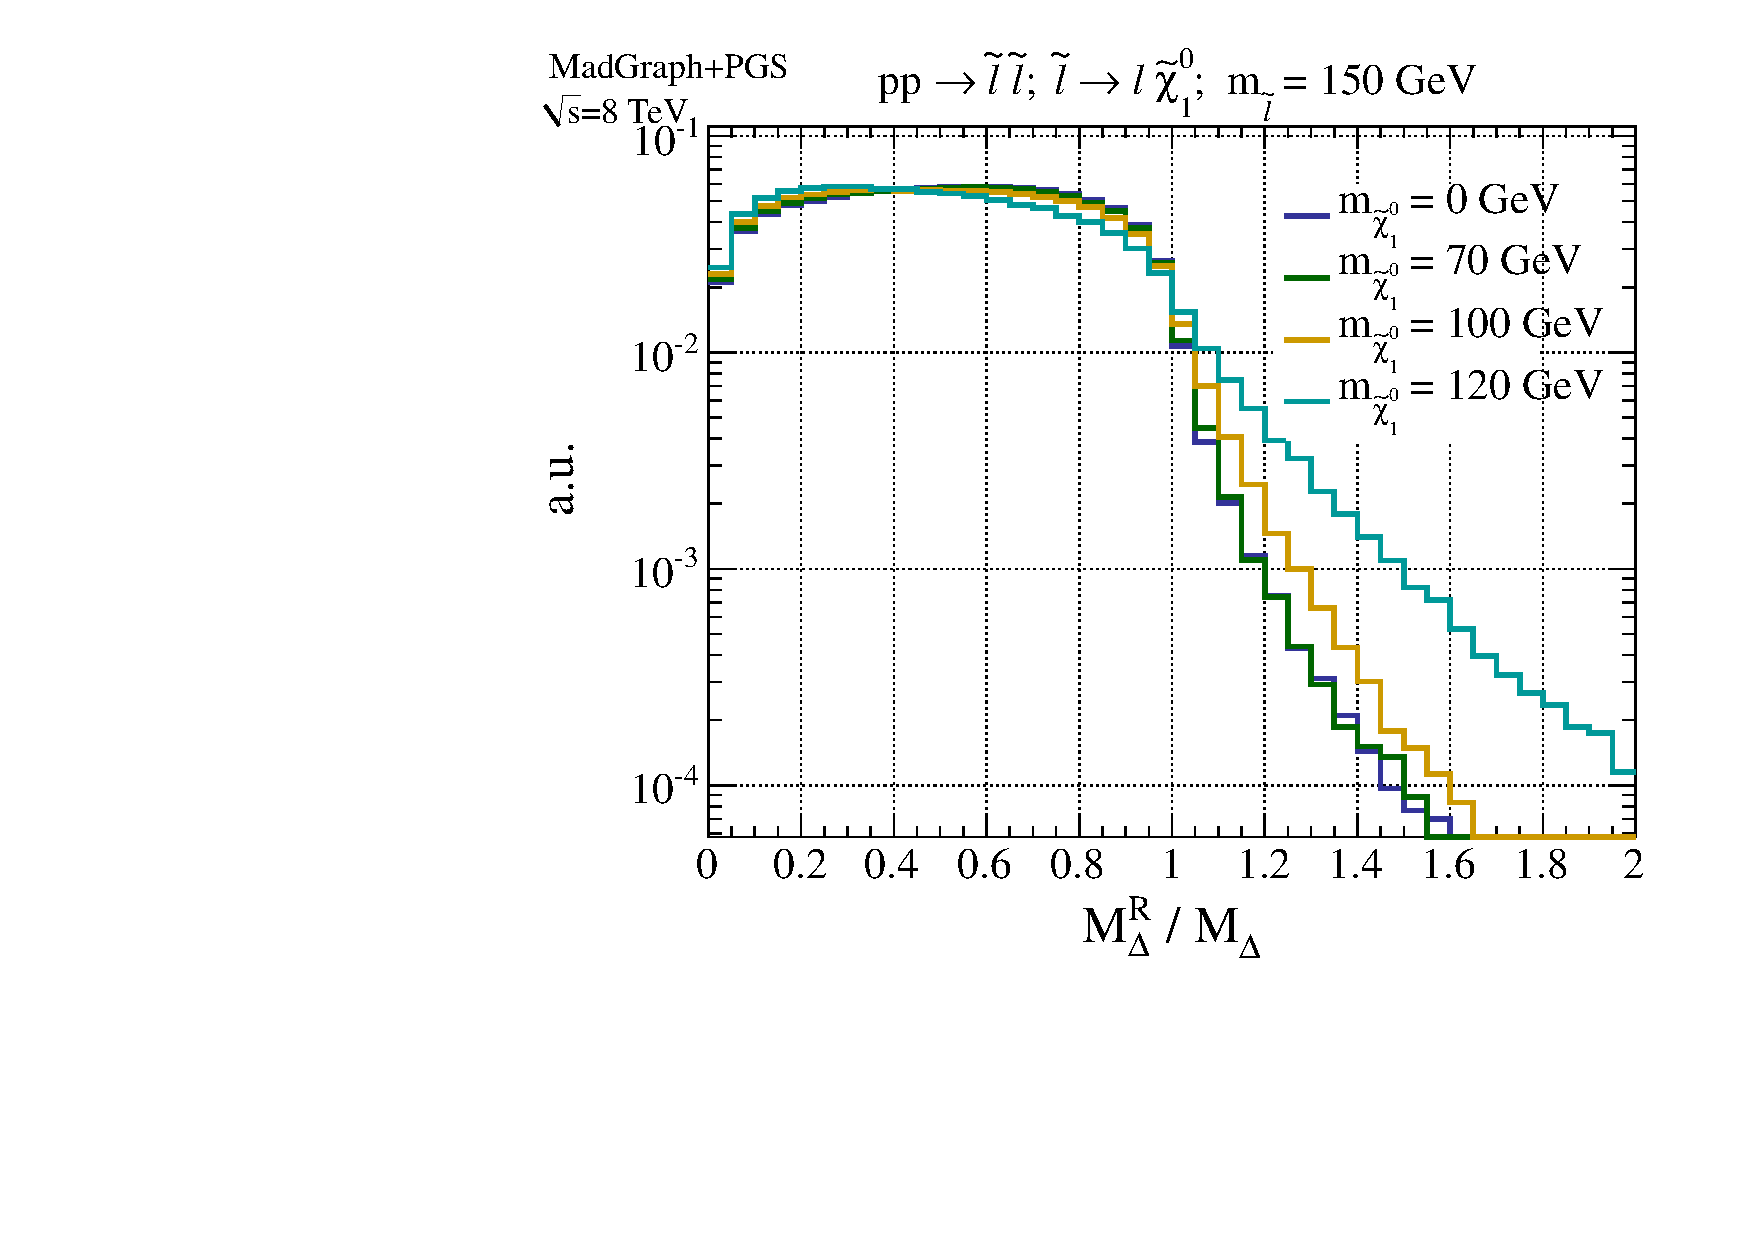
\includegraphics[width=0.3\columnwidth]{fig/sectionIII/Mdelta_norm_log_1D_slepton.pdf}
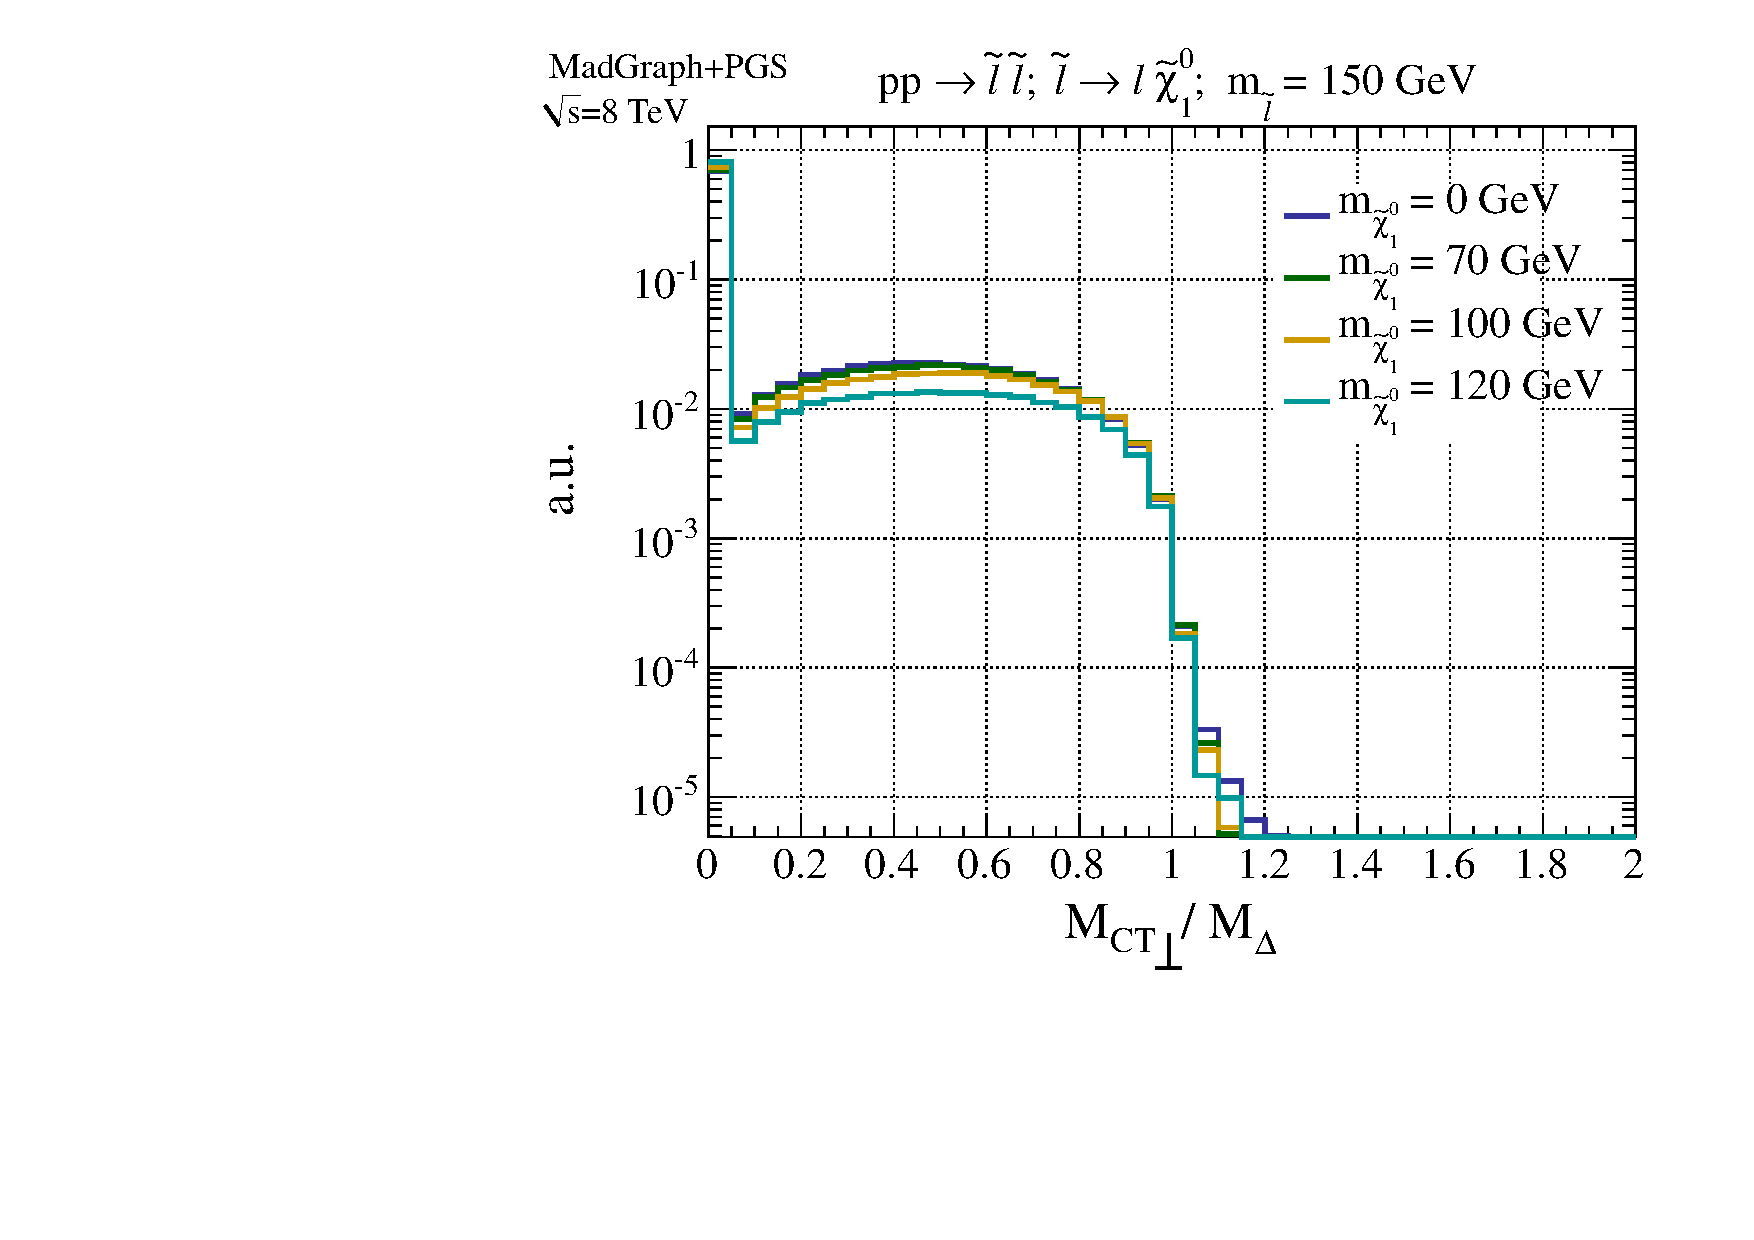
\includegraphics[width=0.3\columnwidth]{fig/sectionIII/MCTperp_norm_log_1D_slepton.pdf} 
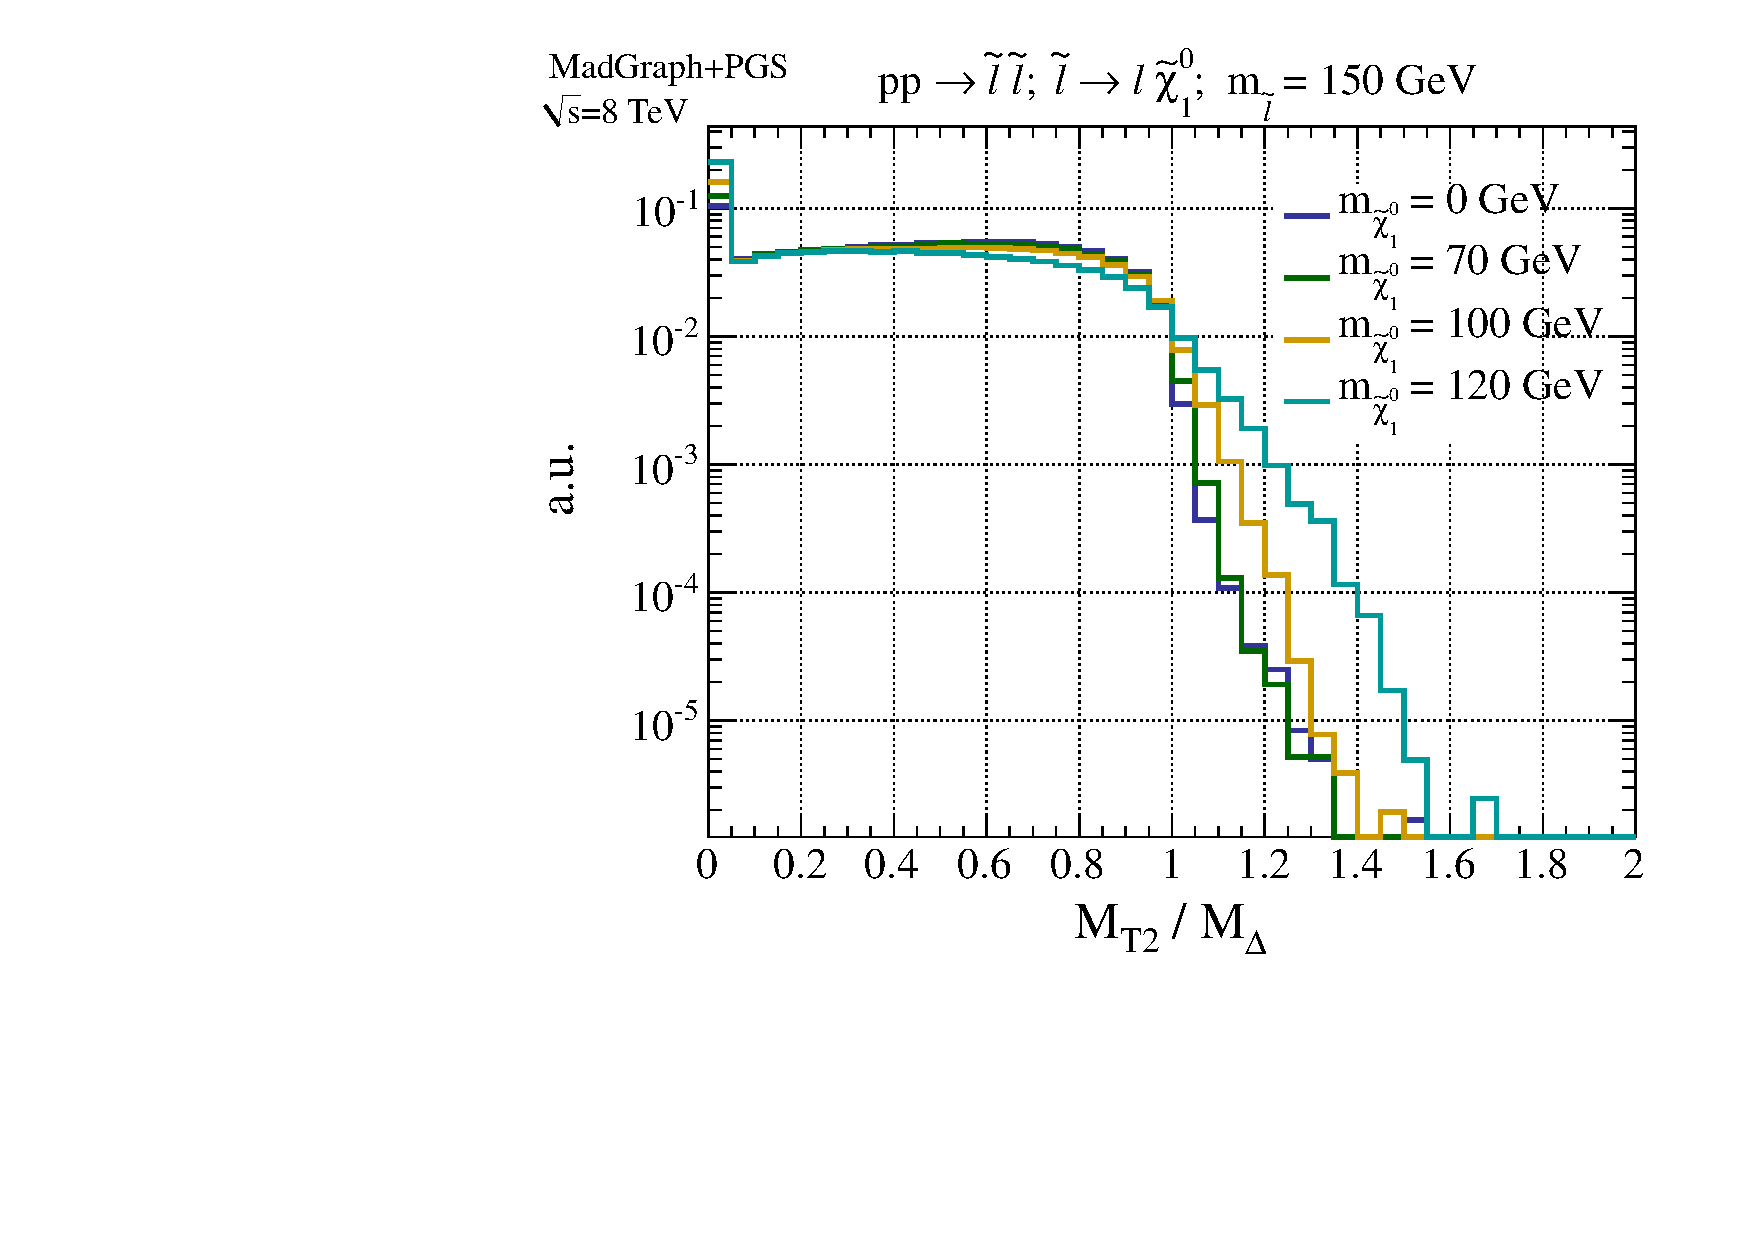
\includegraphics[width=0.3\columnwidth]{fig/sectionIII/MT2_norm_log_1D_slepton.pdf} 
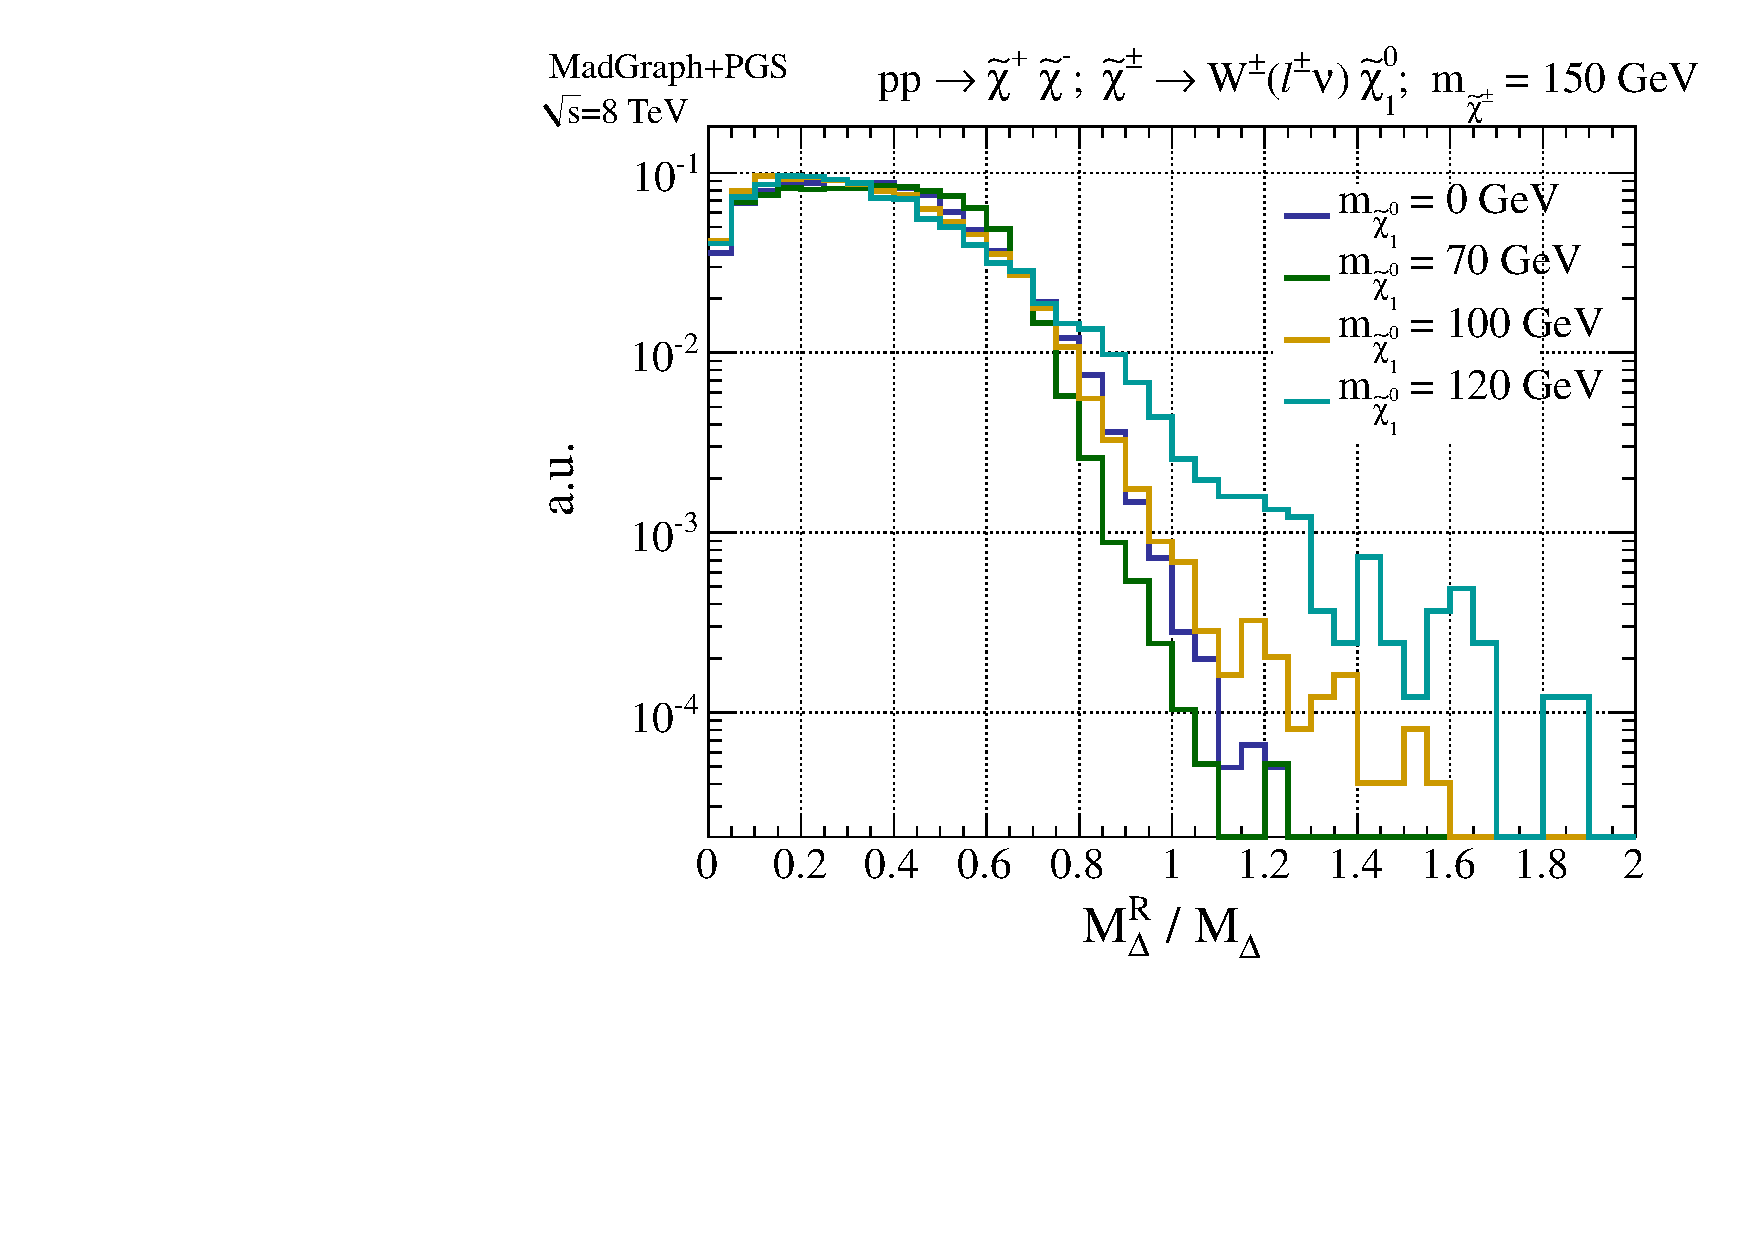
\includegraphics[width=0.3\columnwidth]{fig/sectionIII/Mdelta_norm_log_1D_chargino.pdf}
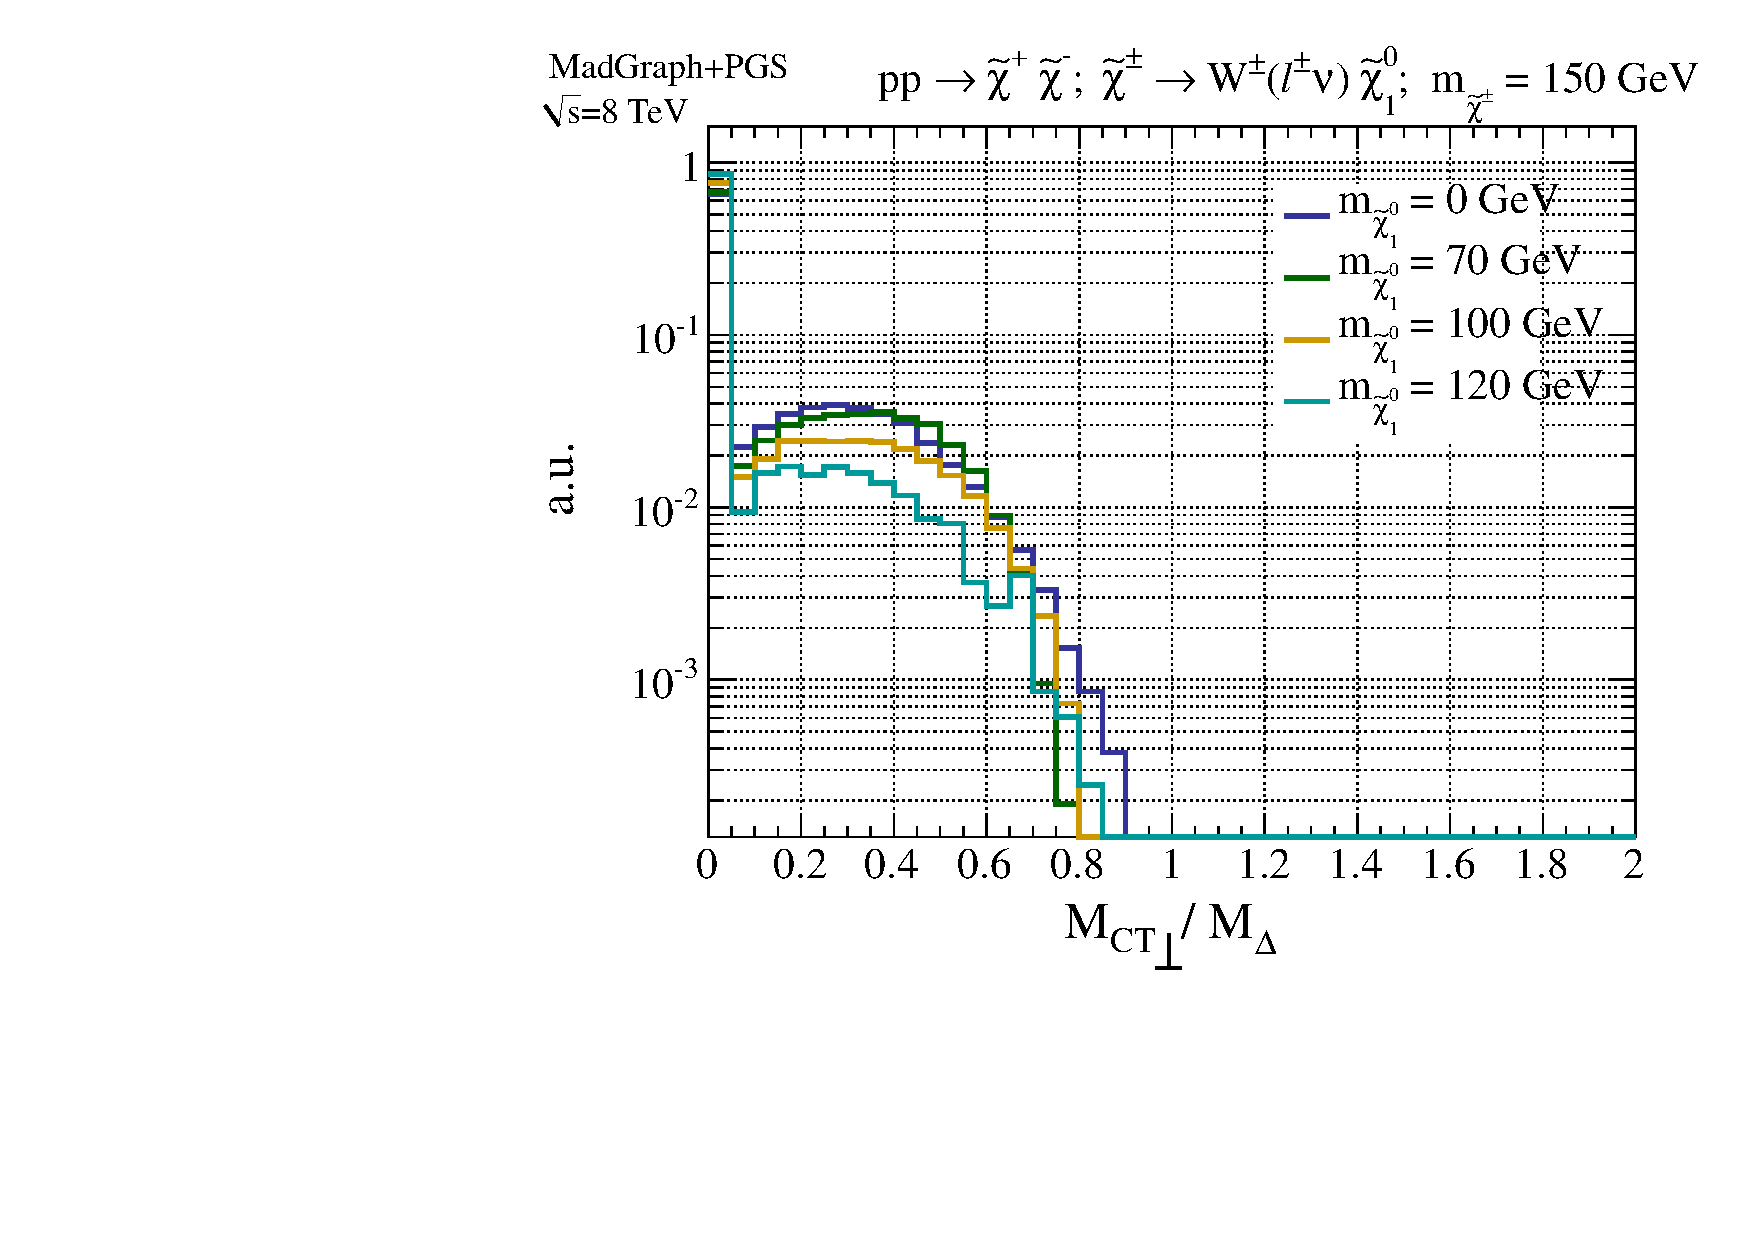
\includegraphics[width=0.3\columnwidth]{fig/sectionIII/MCTperp_norm_log_1D_chargino.pdf} 
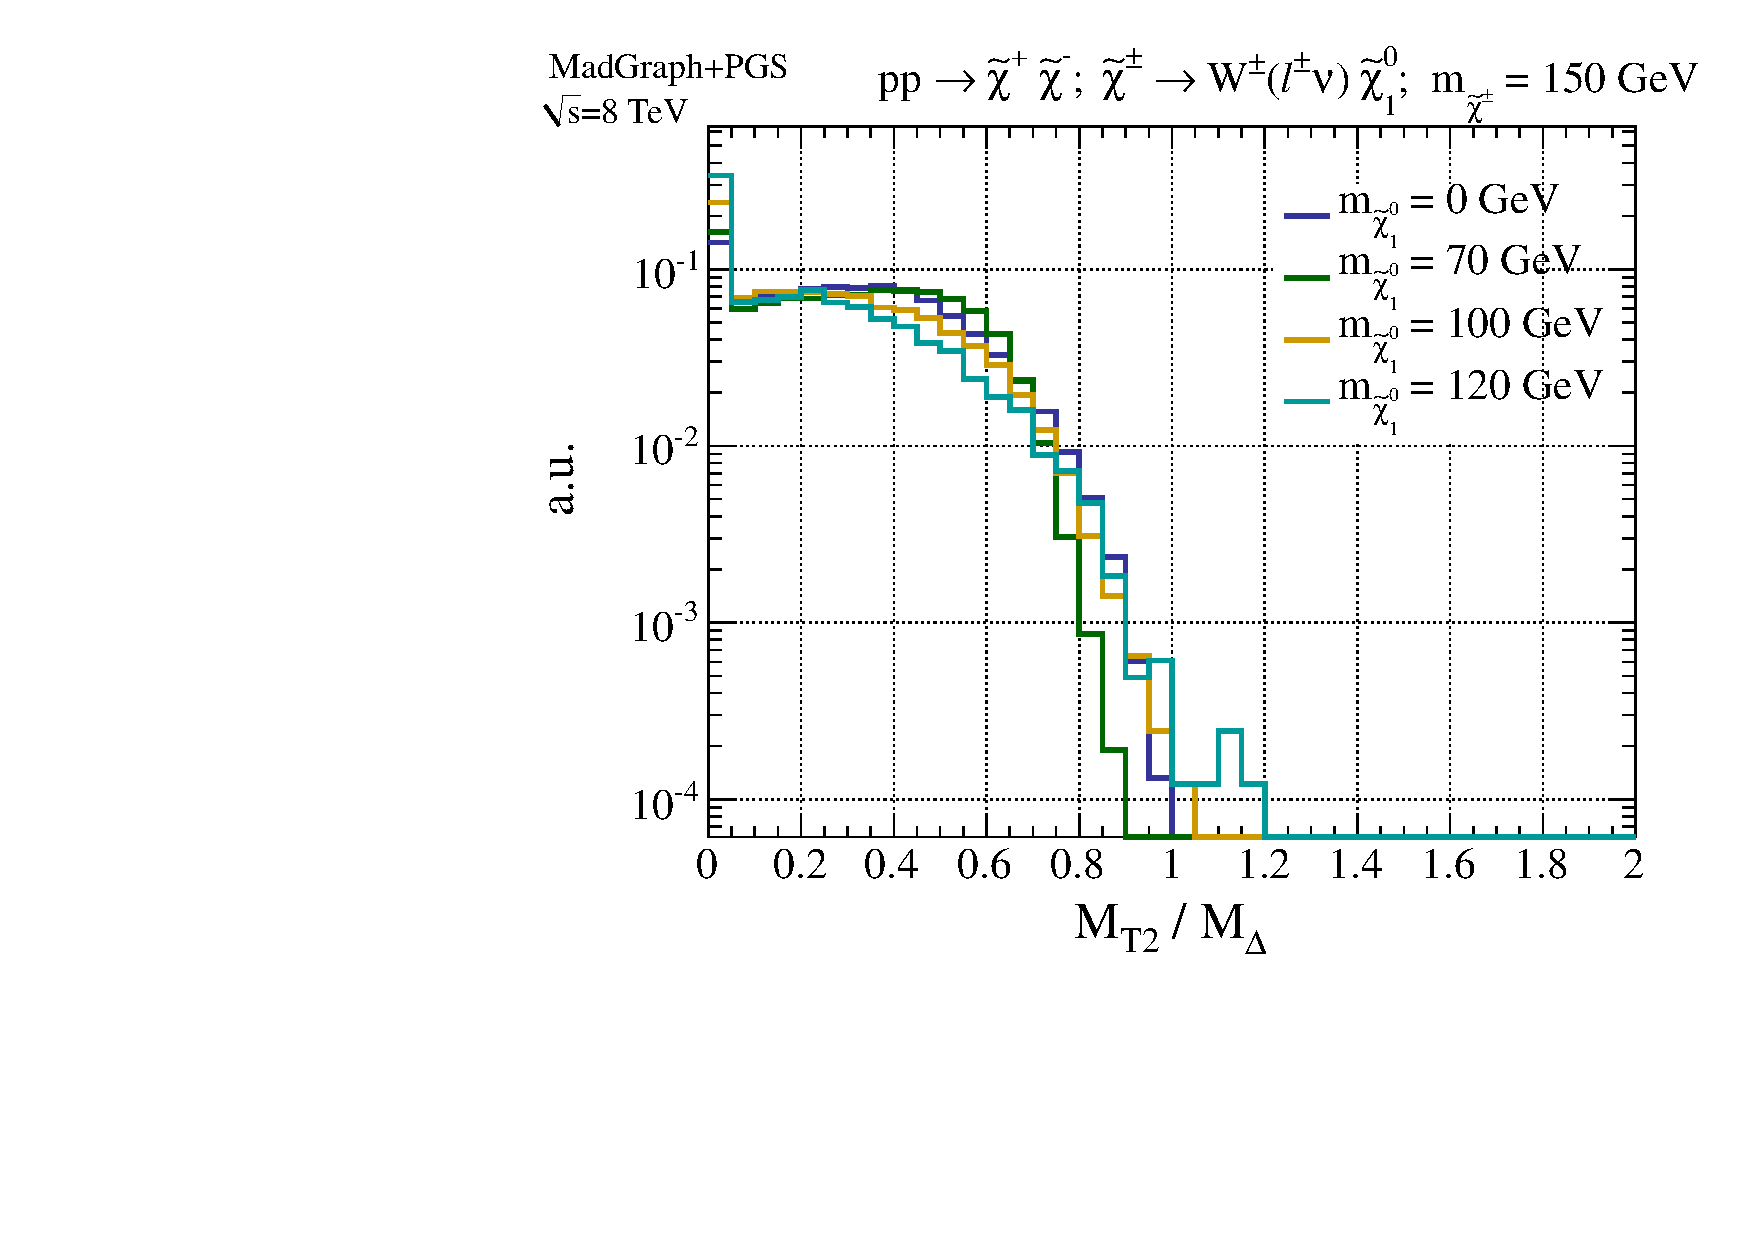
\includegraphics[width=0.3\columnwidth]{fig/sectionIII/MT2_norm_log_1D_chargino.pdf} 
\caption{Distributions of $M_{\Delta}$ estimating variables for sleptons (top row) and charginos (bottom row) with mass 150~GeV decaying into neutralinos and leptons, for a range of neutralino masses. Variables include $M_{\Delta}^{R}$ (left), $M_{CT\perp}$ (center) and $M_{T2}$ (right), all normalized to the true value of $M_{\Delta}$ for each sample. \label{fig:compare}}
\end{figure}

An important property of $M_{CT\perp}$ and $M_{T2}$ is their almost complete insensitivity to the transverse momenta of the di-sparticle CM frame ($p_{T}^\text{CM}$) in these events. Regardless of the velocity of the sparticles in the laboratory frame, the position of the $M_{\Delta}$ endpoint in these distributions remains largely unchanged. This property is convenient for interpretation of the putative signal distributions and essential in the construction of these searches, since it also guarantees the invariance of the same kinematic feature for backgrounds like $WW$ and $t\bar{t}$, even for large $p_{T}^\text{CM}$.  For $M_{T2}$, under-constrained kinematic degrees of freedom are assigned through minimization which removes the $p_{T}^\text{CM}$ dependence. Meanwhile, $M_{CT\perp}$ considers only the lepton kinematics along the transverse axis perpendicular to $\vec{p}_{T}^\text{\, CM}$, largely ignoring variations which are sensitive to its magnitude. 

For $M_{\Delta}^{R}$ the same behavior is achieved by explicitly correcting for non-zero $p_{T}^\text{CM}$, transforming the di-lepton system from the laboratory frame to an approximation of the CM frame. By using only Lorentz invariant information in the determination of this transformation, the definition of the resulting reference frame is stable under variations of $p_{T}^\text{CM}$, as are kinematic variables (such as $M_{\Delta}^{R}$) evaluated in it. From Figure~\ref{fig:compare} is clear that the endpoint behavior of these $M_{\Delta}$ estimators has only mild sensitivity to the choice of strategy for removing $p_{T}^\text{CM}$ dependence. 

However, this choice does effect which events can be used to gain sensitivity to $M_{\Delta}$, as can be seen in the presence or absence of an accumulation of events with a value of zero for each of these discriminants. By only considering information along one transverse axis in the event, $M_{CT\perp}$ is exactly zero around 50\% of the time, corresponding to cases where the two leptons are moving in opposite directions along that axis. $M_{T2}$ exhibits similar behavior, though with fewer events having $M_{T2} = 0$. This fraction of events are observed to vary with different signal mass combinations, and also with the magnitude of $p_{T}^\text{CM}$ (see Figure~\ref{fig:compare}). This latter dependence can be seen by comparing the $M_{T2}$ distribution between different jet multiplicity categories, as shown in Figure~\ref{fig:compare_njet}, for each of the three $M_{\Delta}$ estimators, whereby larger jet multiplicity is generally correlated with larger $p_{T}^\text{CM}$. We observe that $M_{\Delta}^{R}$ does not exhibit this behavior.

\begin{figure}[ht]
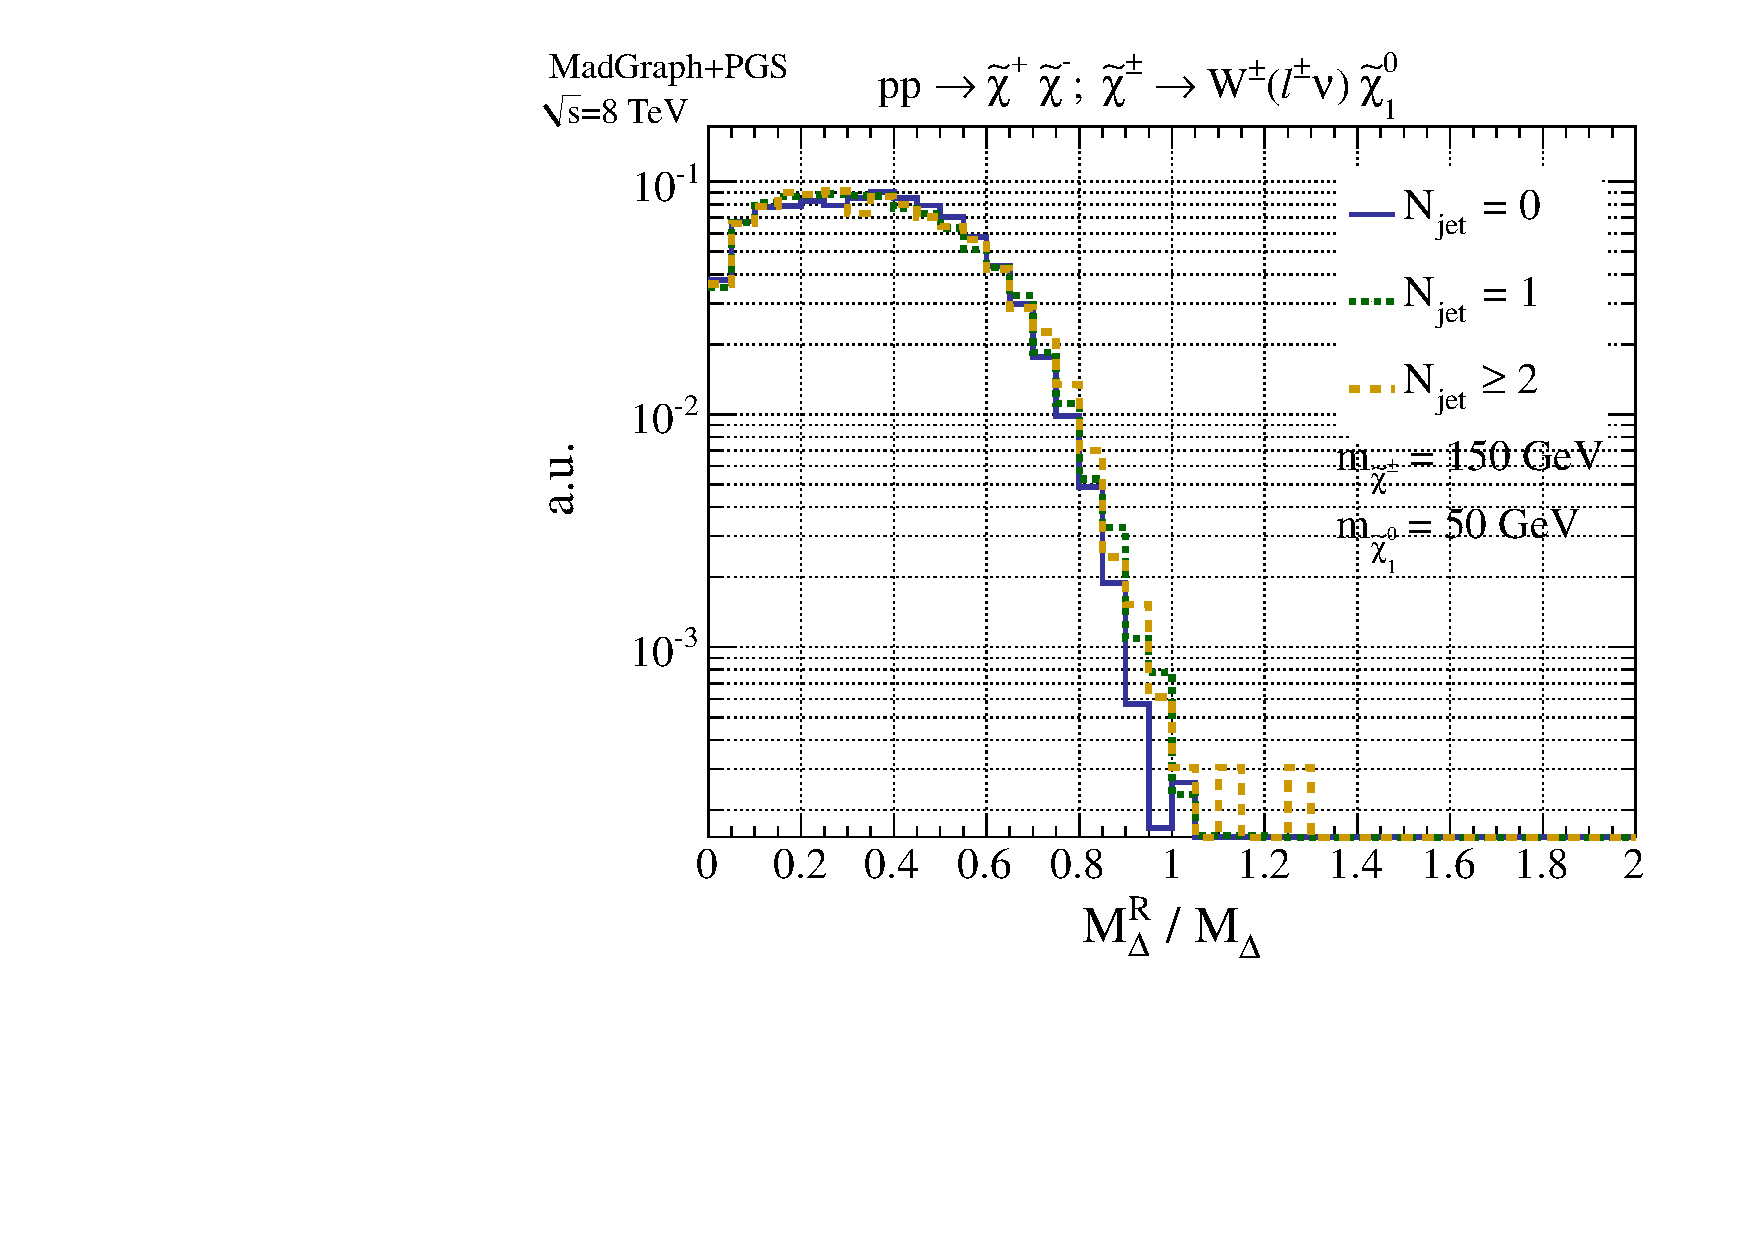
\includegraphics[width=0.3\columnwidth]{fig/sectionIII/Mdelta_norm_Njet_log_chargino.pdf}
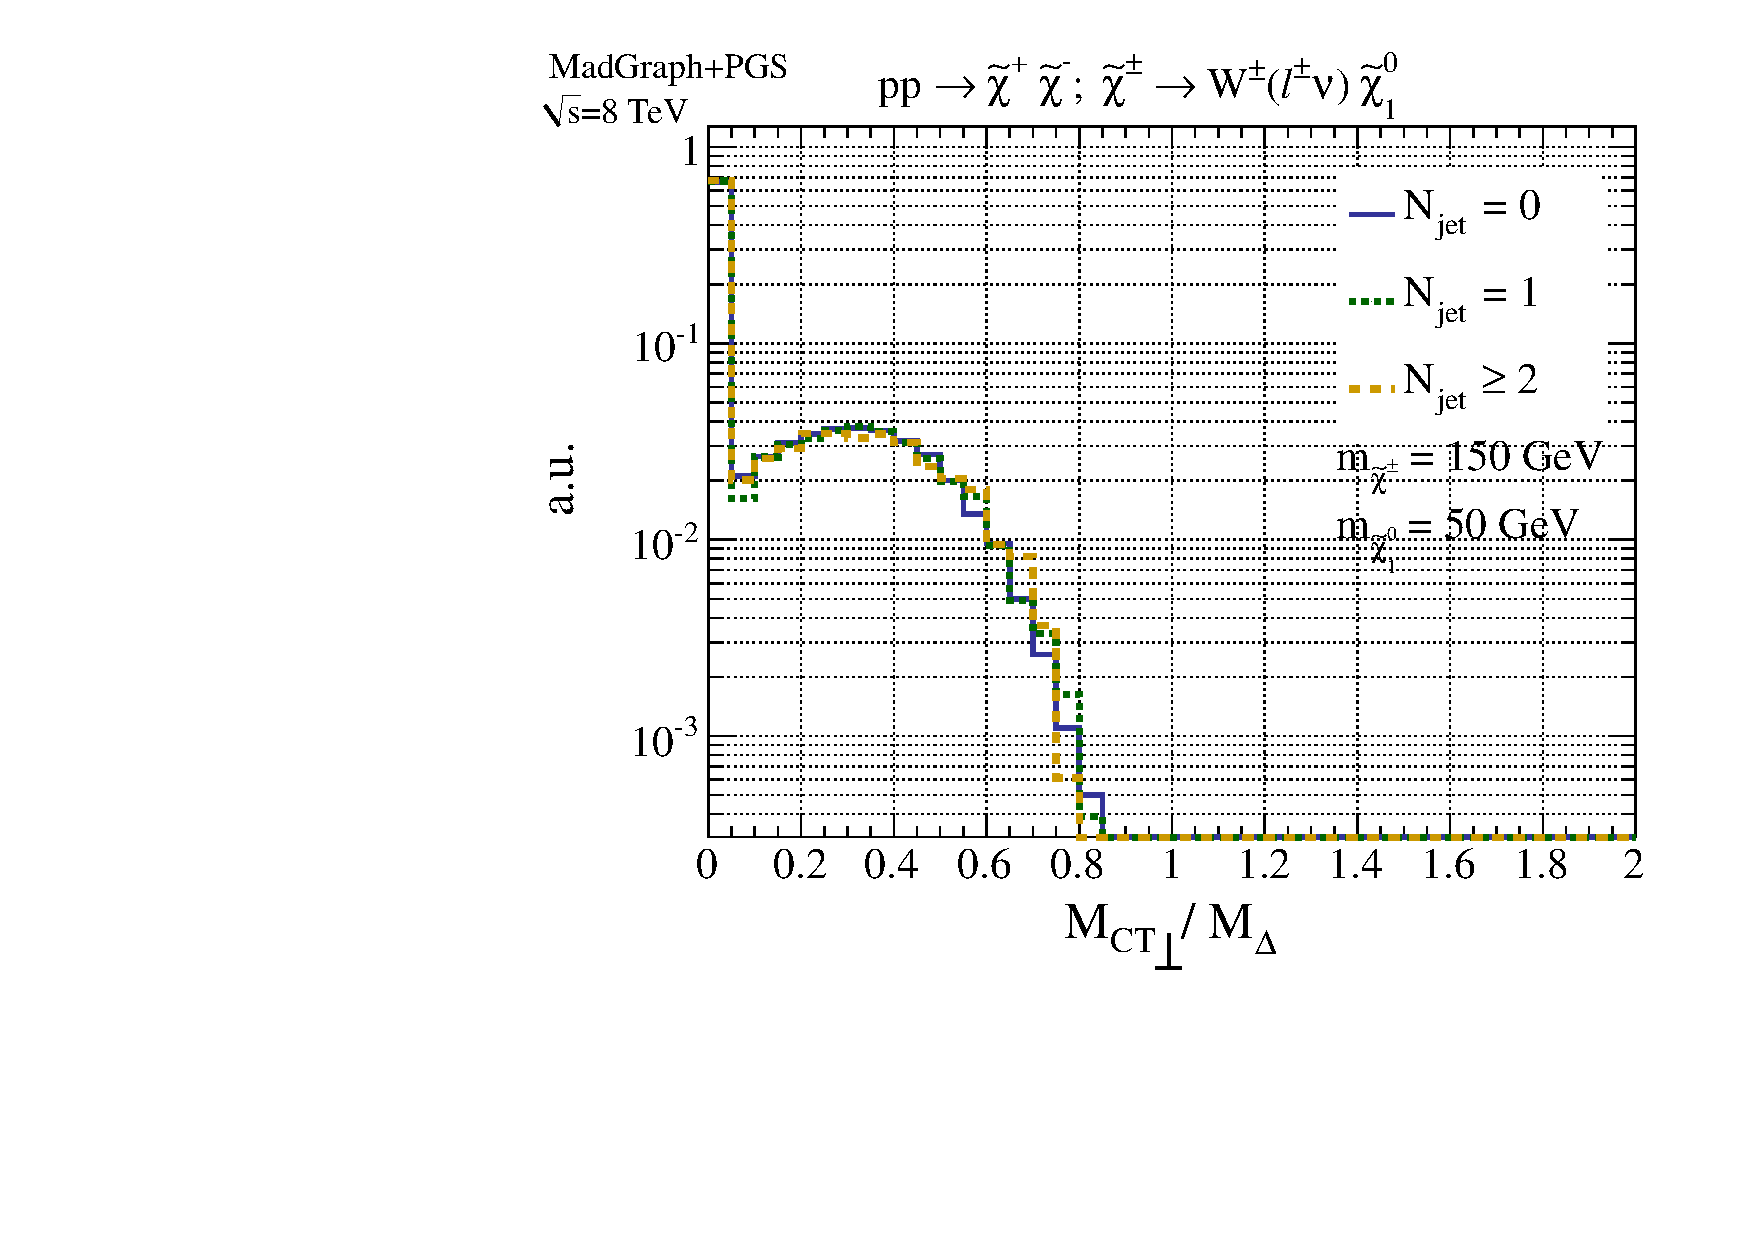
\includegraphics[width=0.3\columnwidth]{fig/sectionIII/MCTperp_norm_Njet_log_chargino.pdf} 
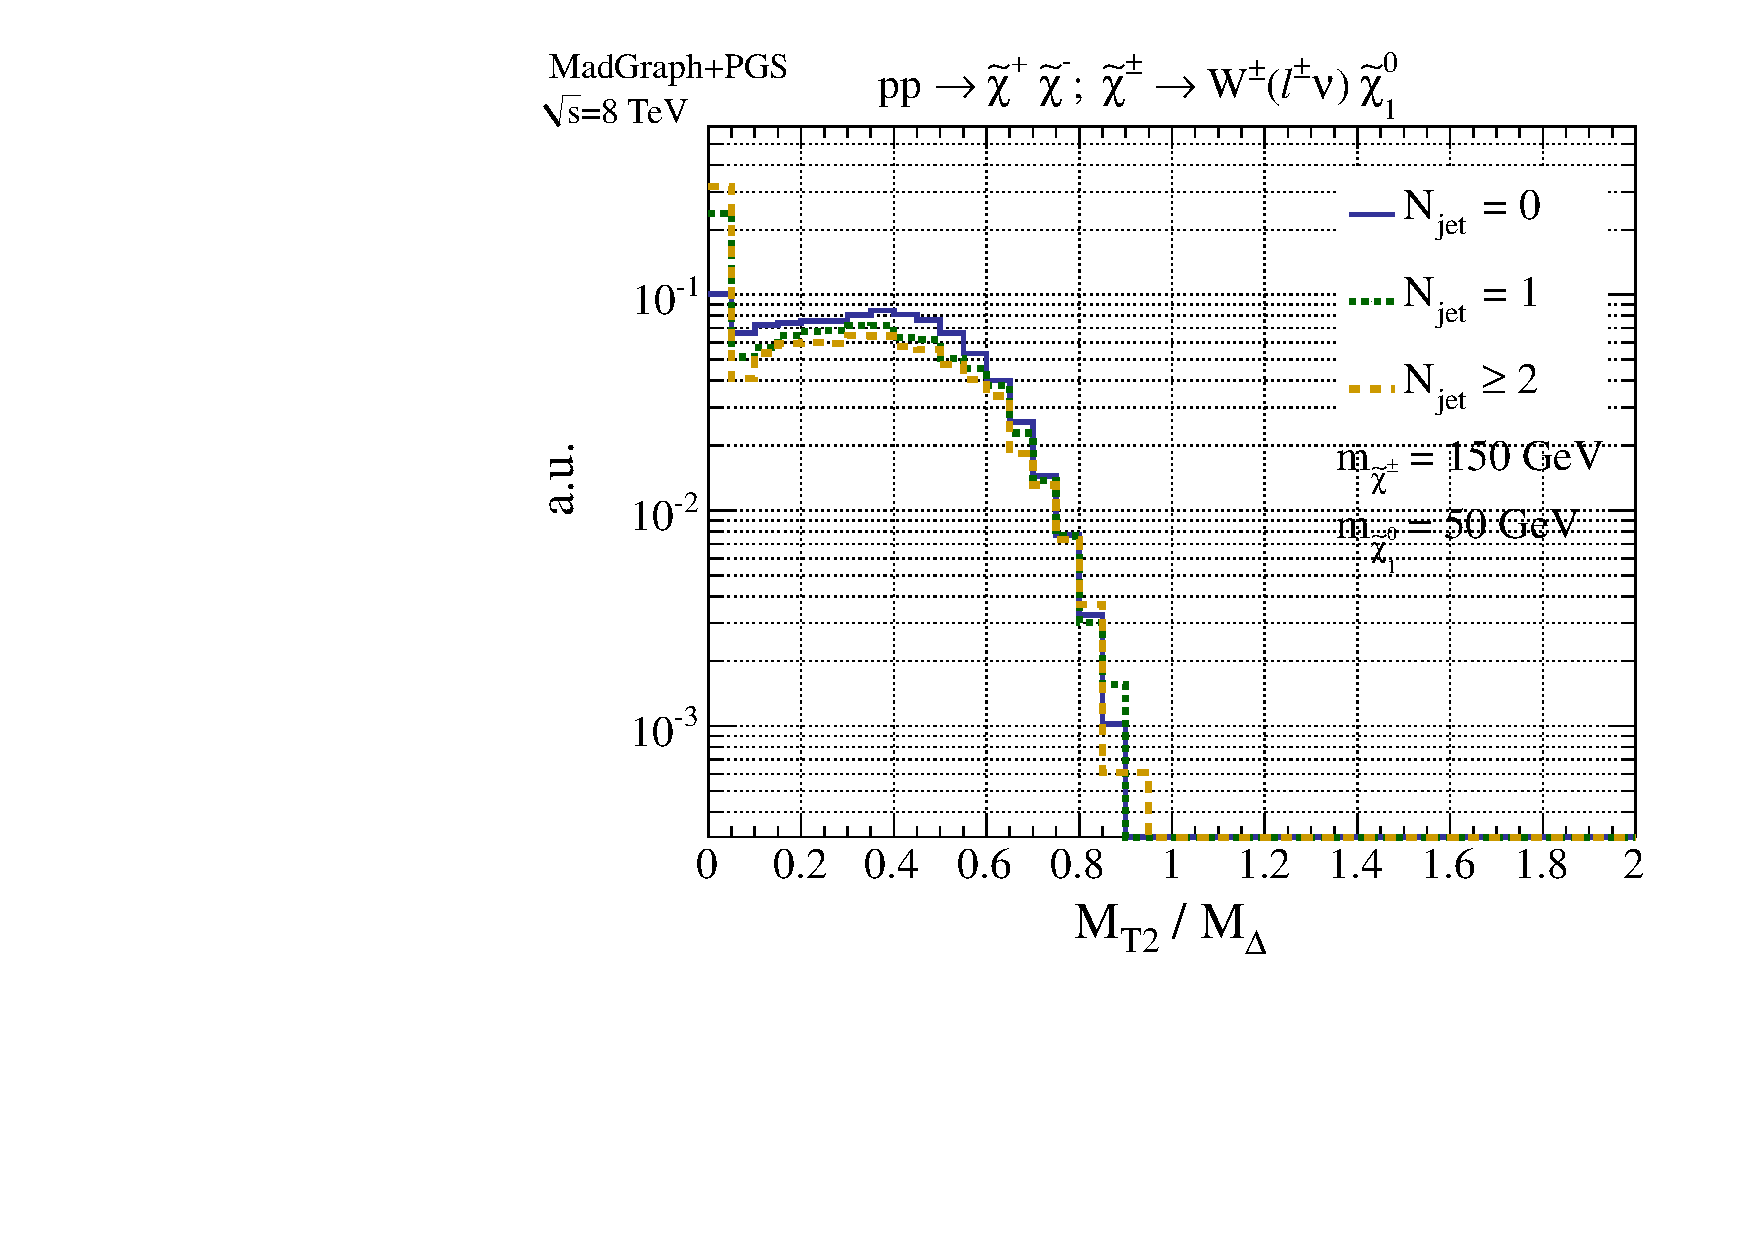
\includegraphics[width=0.3\columnwidth]{fig/sectionIII/MT2_norm_Njet_log_chargino.pdf} 
\caption{Distributions of $M_{\Delta}$ estimating variables for charginos with mass 150~GeV decaying into 50~GeV neutralinos and leptonically decaying $W$ bosons, as a function of reconstructed jet multiplicity. Variables include $M_{\Delta}^{R}$ (left), $M_{CT\perp}$ (center) and $M_{T2}$ (right), all normalized to the true value of $M_{\Delta}$ for each sample. \label{fig:compare_njet}}
\end{figure}

The accumulation of events at zero in any of these kinematic variables has subtle effects on analysis that use them. Since the behavior is similar for both signal and background events, the ratio of the expected yields is largely insensitive to this effect. What does change is the size of the effective dataset that contains information about $M_{\Delta}$. The 50\% of events with $M_{CT\perp} = 0$ means that the integrated luminosity used in a search is effectively halved, while the increasing number of $M_{T2} = 0$ events at larger $p_{T}^\text{CM}$ results in a similar effect for higher jet multiplicities and/or boosted topologies. The quantitative implications of these dependencies on both selection efficiency and ultimately expected sensitivity of searches are discussed in the following sections.

\subsection{CMS and ATLAS-like event selections\label{sec:CMSATLAS}}

At this stage we have only considered kinematic variables in the context of quite inclusive event selections. In practice, searches for new physics in di-lepton final states include multiple kinematic requirements, each designed to suppress particular backgrounds. These additional requirements often involve other discriminating variables, like $E_{T}^\text{miss}$, which can be highly correlated with the $M_{\Delta}$ estimators described in the previous section. Understanding the efficacy of any of these variables depends on the context of where in kinematic phase-space an analysis is searching. In order to evaluate whether using the variable $M_{\Delta}^{R}$ would yield an improvement in the sensitivity of the CMS and ATLAS searches we define CMS- and ATLAS-like event selections through which we attempt to capture the relevant qualitative features of the kinematic requirements enforced in these analyses. 

In addition to the baseline selection requirements described in Section~\ref{sec:baseline} we consider criteria used by CMS and ATLAS (largely designed to reject Drell-Yan backgrounds):\\
\begin{tabular}{c c}
~~~~~~~~~~~~~~~~~~~~~~~~~~~~~~~~{\bf CMS selection}~~~~~~~~~~~~~~~~~~~~~~~~~~~~~~~~ & {\bf ATLAS selection} \\
& \\
$|m(\ell\ell) - m_{Z}| > 15$~GeV (SF channels) & $|m(\ell\ell) - m_{Z}| > 10$~GeV (SF channels) \\
$E_{T}^\text{miss} > 60$~GeV & $E_{T}^\text{miss,rel} > 40$~GeV
\end{tabular}

where
\begin{eqnarray}      
E_{T}^\text{miss,rel} = \left\{
	\begin{array}{l l}
	E_{T}^\text{miss}  & \quad \mathrm{if}~\sin\Delta\phi_{\ell,j} \ge \pi/2~, \\
	E_{T}^\text{miss} \times \sin\Delta\phi_{\ell,j} & \quad \mathrm{if}~\sin\Delta\phi_{\ell,j} < \pi/2~,
	\end{array} \right. 
	\label{eq:function}
\end{eqnarray} 
and $\Delta\phi_{\ell,j}$ is the azimuthal angle between the lepton or jet closest in the transverse plane to $\vec{E}_{T}^\text{miss}$. Topologically, backgrounds like $WW$ and $t\bar{t}$ are similar to the slepton and chargino signals, with two massive $W$ bosons each decaying to a lepton and neutrino. As a result, the searches' ability to distinguish signal events from these backgrounds is dependent mostly on the difference between $m_{W}$ and $M_{\Delta}$ of each signal, and is accomplished primarily through kinematic variables estimating $M_{\Delta}$. The CMS and ATLAS selection requirements listed above are added specifically to reject $Z/\gamma^*$+jets events, using a $Z$ mass window veto and $E_{T}^\text{miss}$ related selections to eliminate events with mis-measured jets or leptons which result in spurious $E_{T}^\text{miss}$. 

The CMS and ATLAS selection efficiencies for sleptons and charginos, as a function of sparticle masses, are summarized in Figure~\ref{fig:EFF_inclusive}. Without explicit requirements placed on $M_{\Delta}$-estimating variables, the selection efficiencies are relatively flat throughout most of the sparticle mass parameter-space, dropping quickly as parent sparticles and neutrinos approach mass degeneracy. This efficiency drop is a result of portions of the event selection involving energy scale, in this case minimum lepton $p_{T}$ requirements and $E_{T}^\text{miss}$/$E_{T}^\text{miss,rel}$ cuts. For di-slepton production, the leptons are produced in two-body decays of the parent sparticle resulting in the lepton and neutralino momentum distributions scaling closely with $M_{\Delta}$ and a large efficiency gradient once energy scale requirements become comparable to the sparticle mass difference. For chargino models this gradient is less dramatic; with leptons produced in subsequent decays of $W$ bosons (rather than in two-body decays of sparticles) the momentum distributions are broader, with weaker $M_{\Delta}$ correspondence. Furthermore, neutralinos are not the only weakly interacting particles in the final state and the total momentum of the entire system of weakly interacting particles is smaller as more energy is contained in the mass rather than the momentum. The result is that $E_{T}^\text{miss}$ requirements can be especially inefficient for these signals relative to sleptons, with large drops in efficiency extending further from the mass degeneracy diagonal.

\begin{figure}[ht]
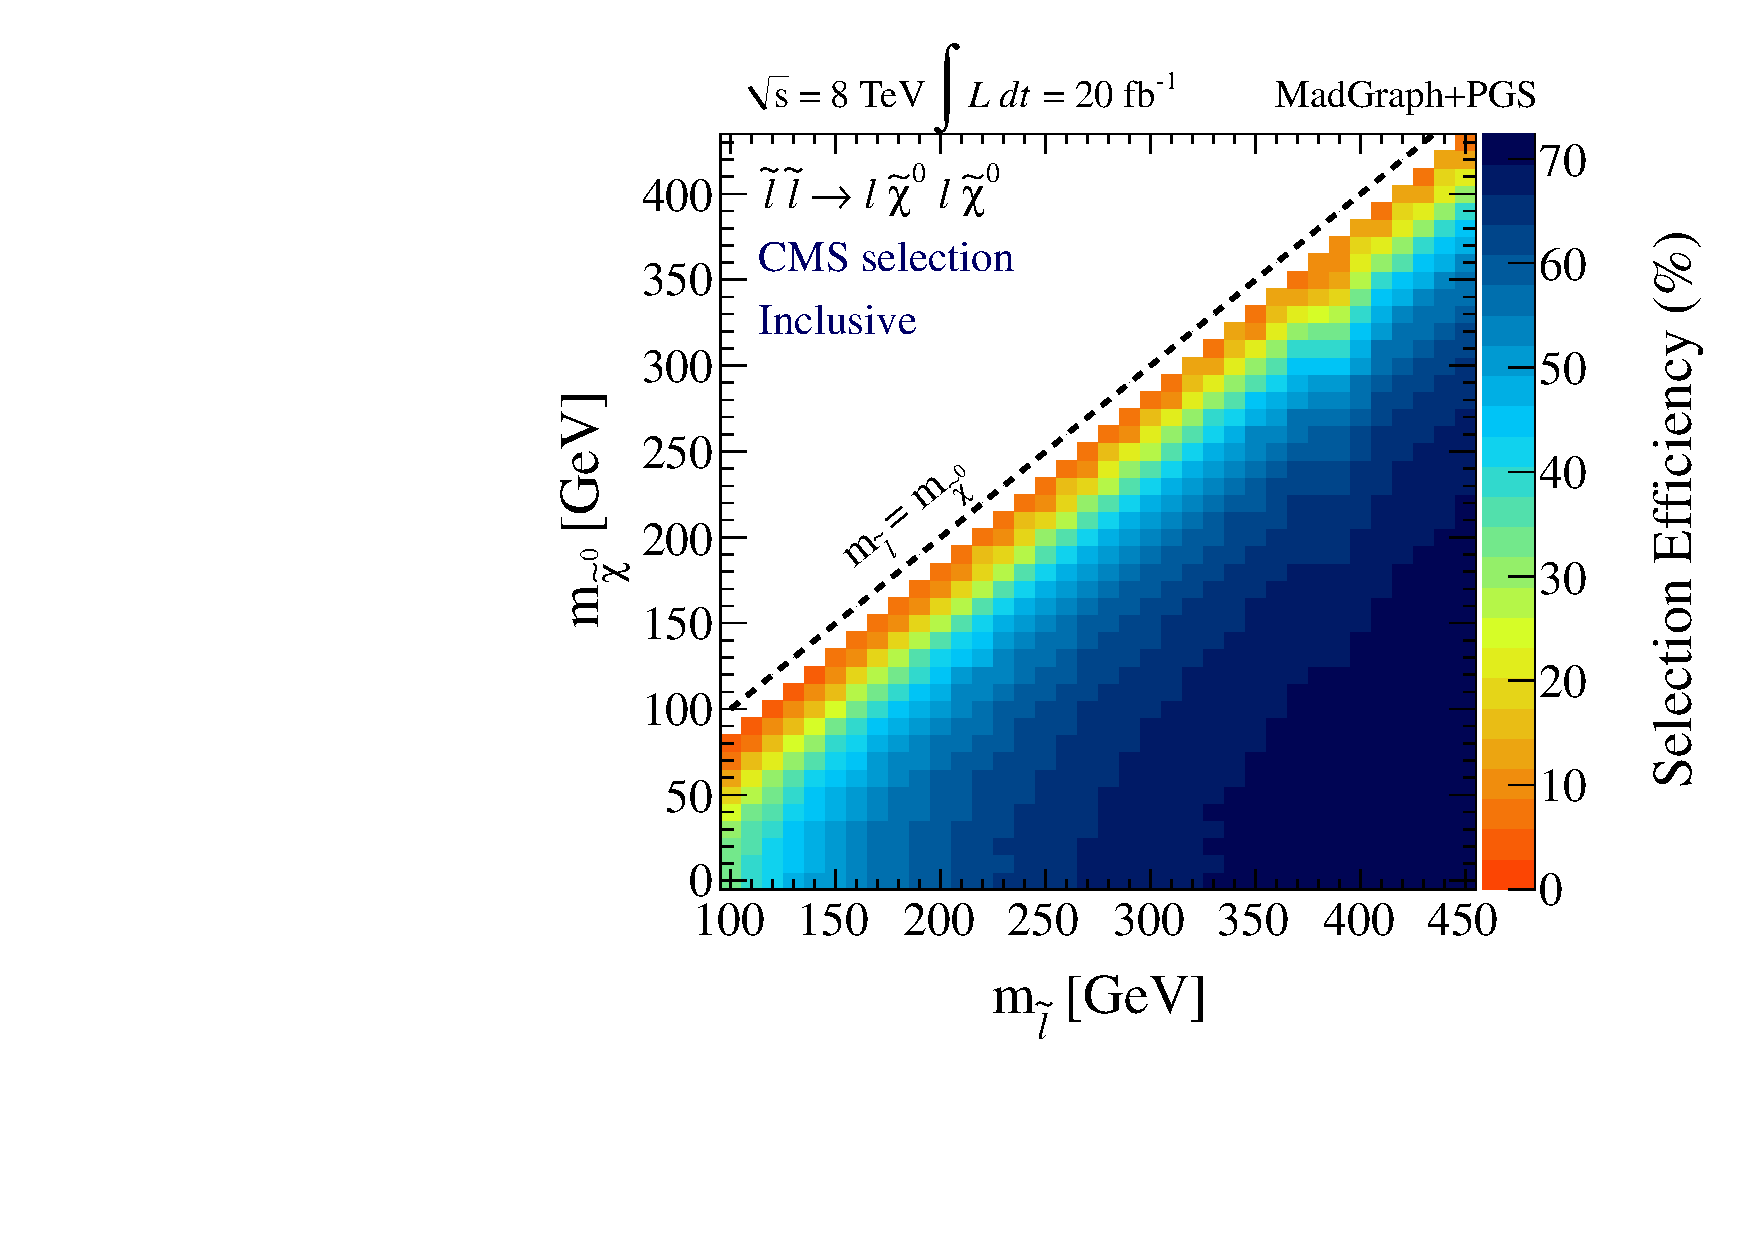
\includegraphics[width=0.35\columnwidth]{fig/sectionIII/EFF_slepton_CMS_incl.pdf}
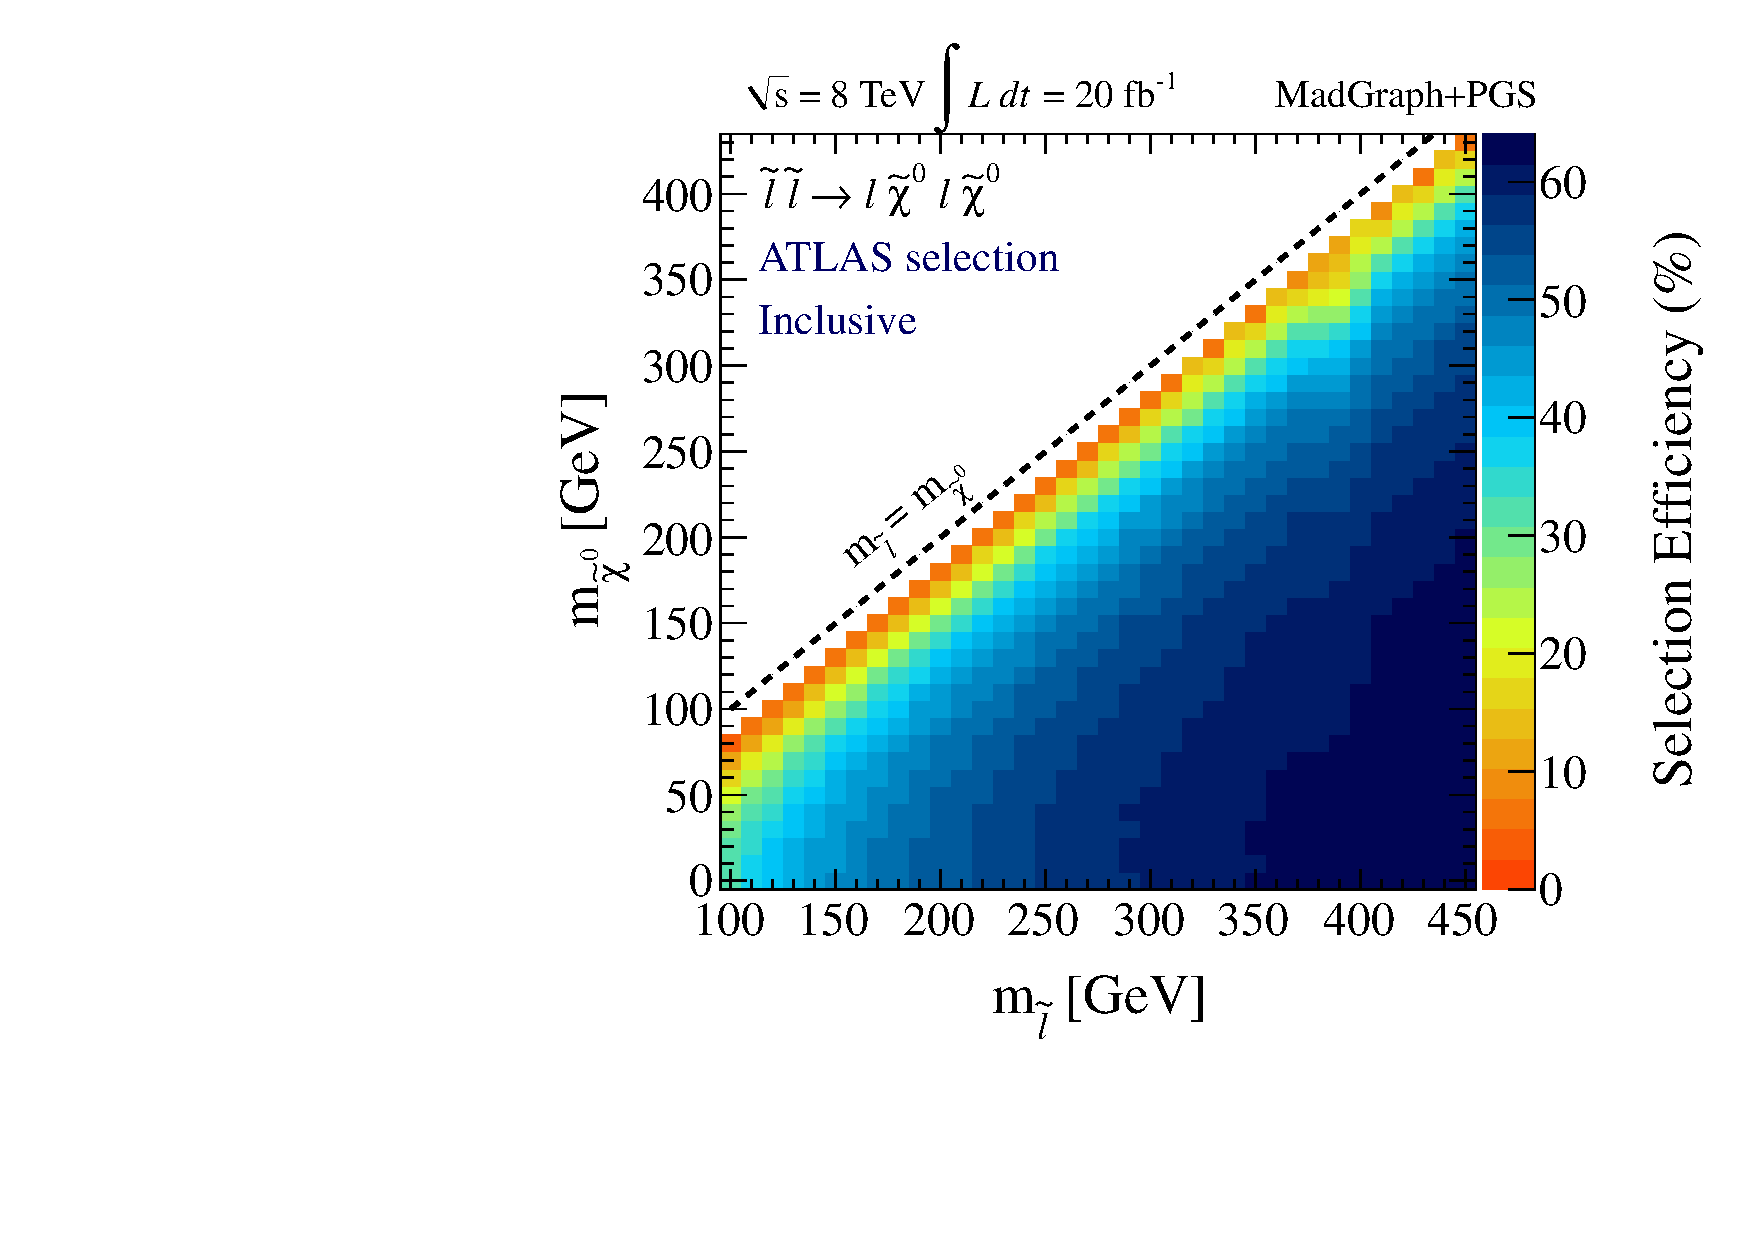
\includegraphics[width=0.35\columnwidth]{fig/sectionIII/EFF_slepton_ATLAS_incl.pdf}\\
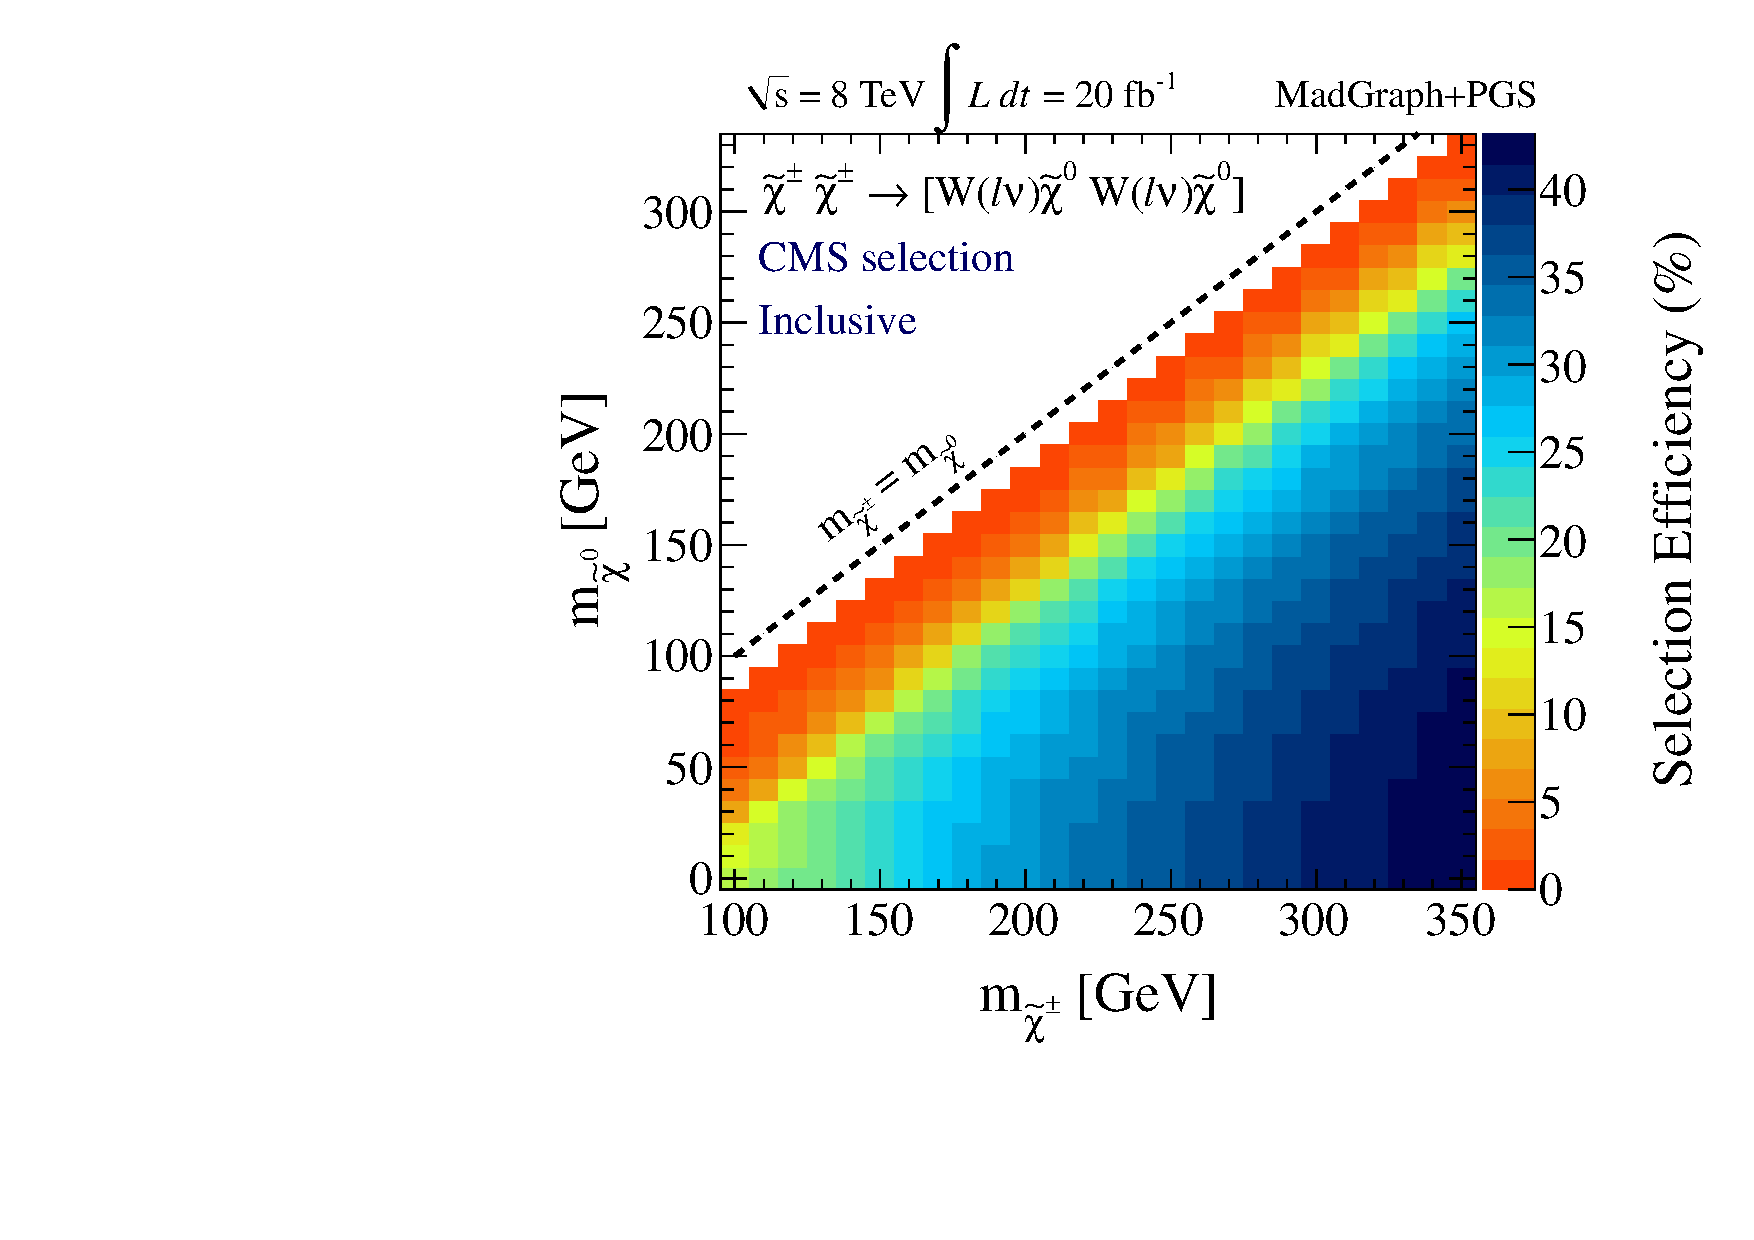
\includegraphics[width=0.35\columnwidth]{fig/sectionIII/EFF_chargino_CMS_incl.pdf}
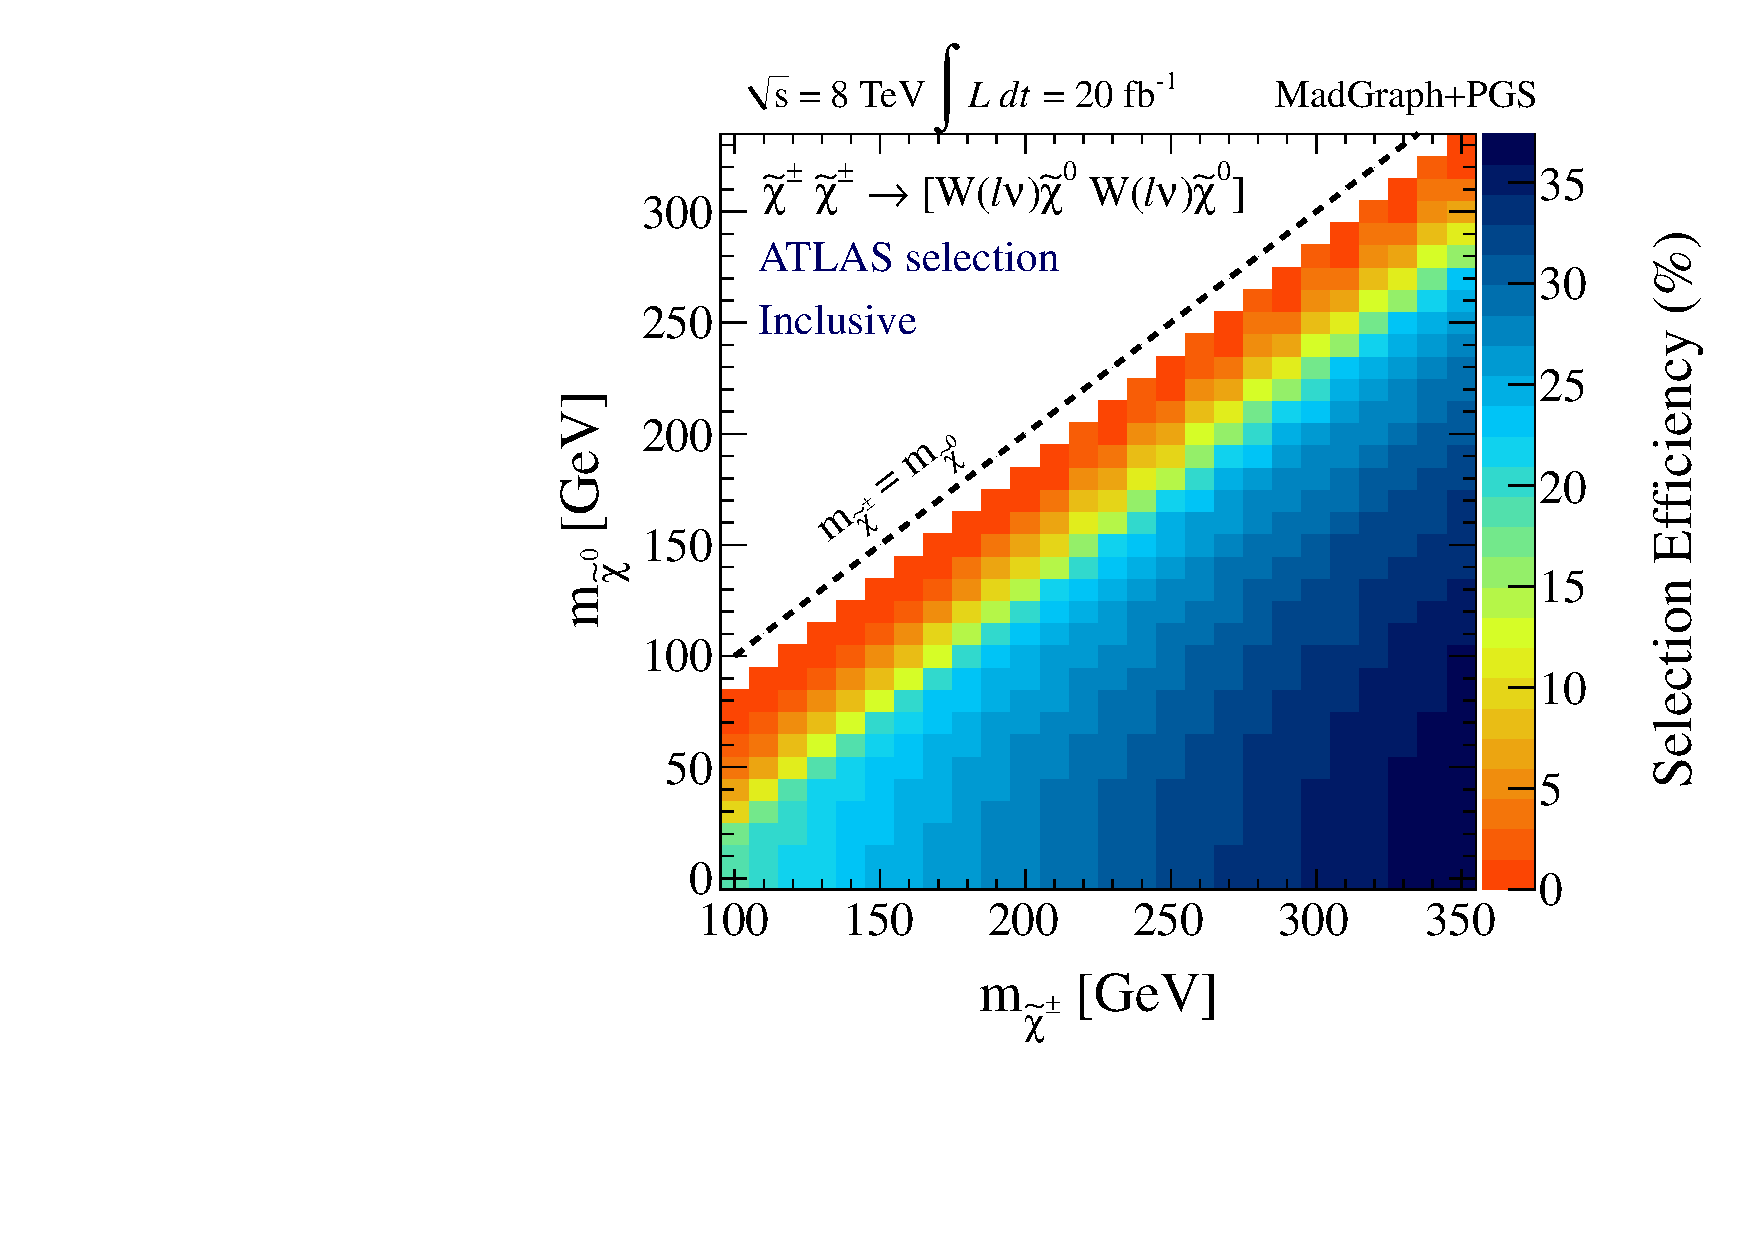
\includegraphics[width=0.35\columnwidth]{fig/sectionIII/EFF_chargino_ATLAS_incl.pdf}
\caption{Efficiency of the CMS (left) and ATLAS (right) selections for the slepton (top) and chargino (bottom) signal models. Selection efficiencies are calculated as a function of parent sparticle and neutralino mass and include all final state categories. \label{fig:EFF_inclusive}}
\end{figure}

\begin{figure}[ht]
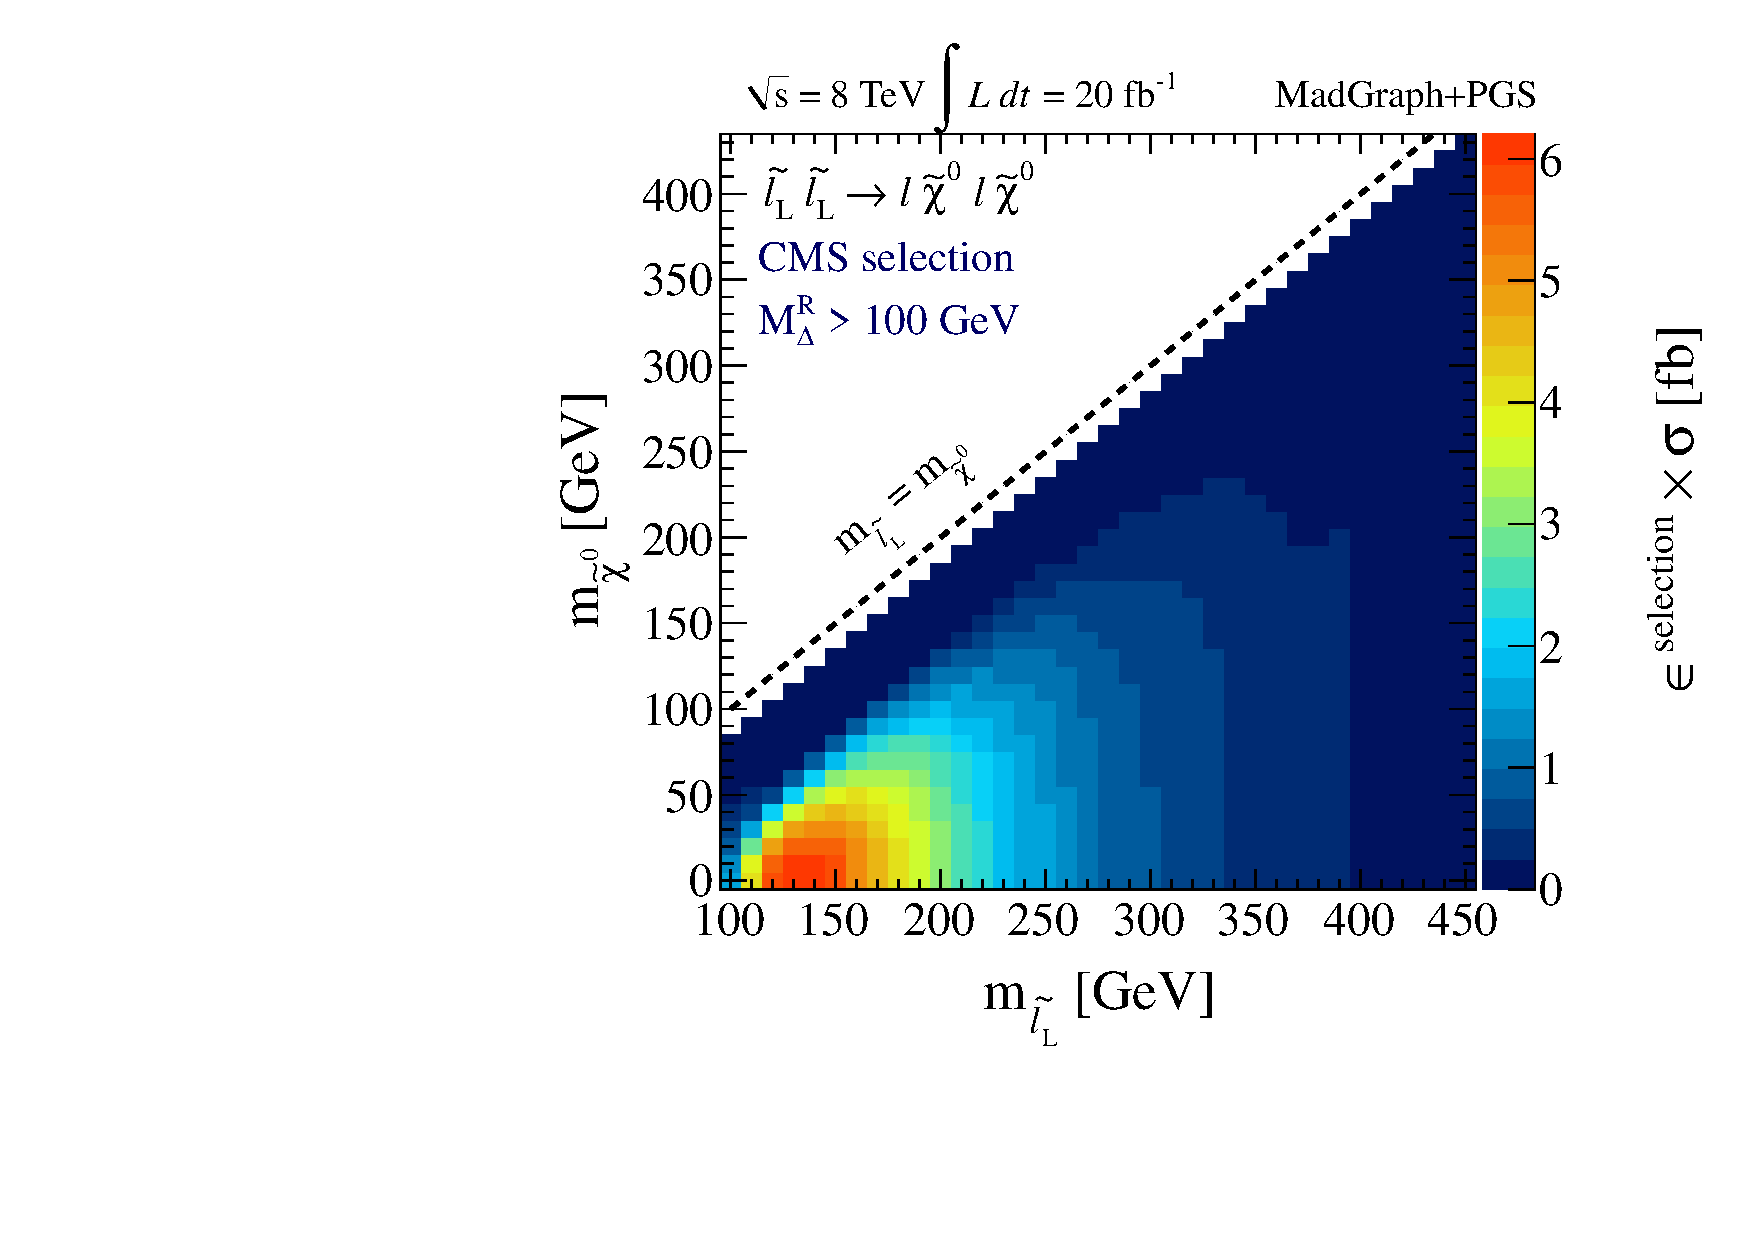
\includegraphics[width=0.35\columnwidth]{fig/sectionIII/XSEC_sleptonL_CMS_Mdelta100.pdf}
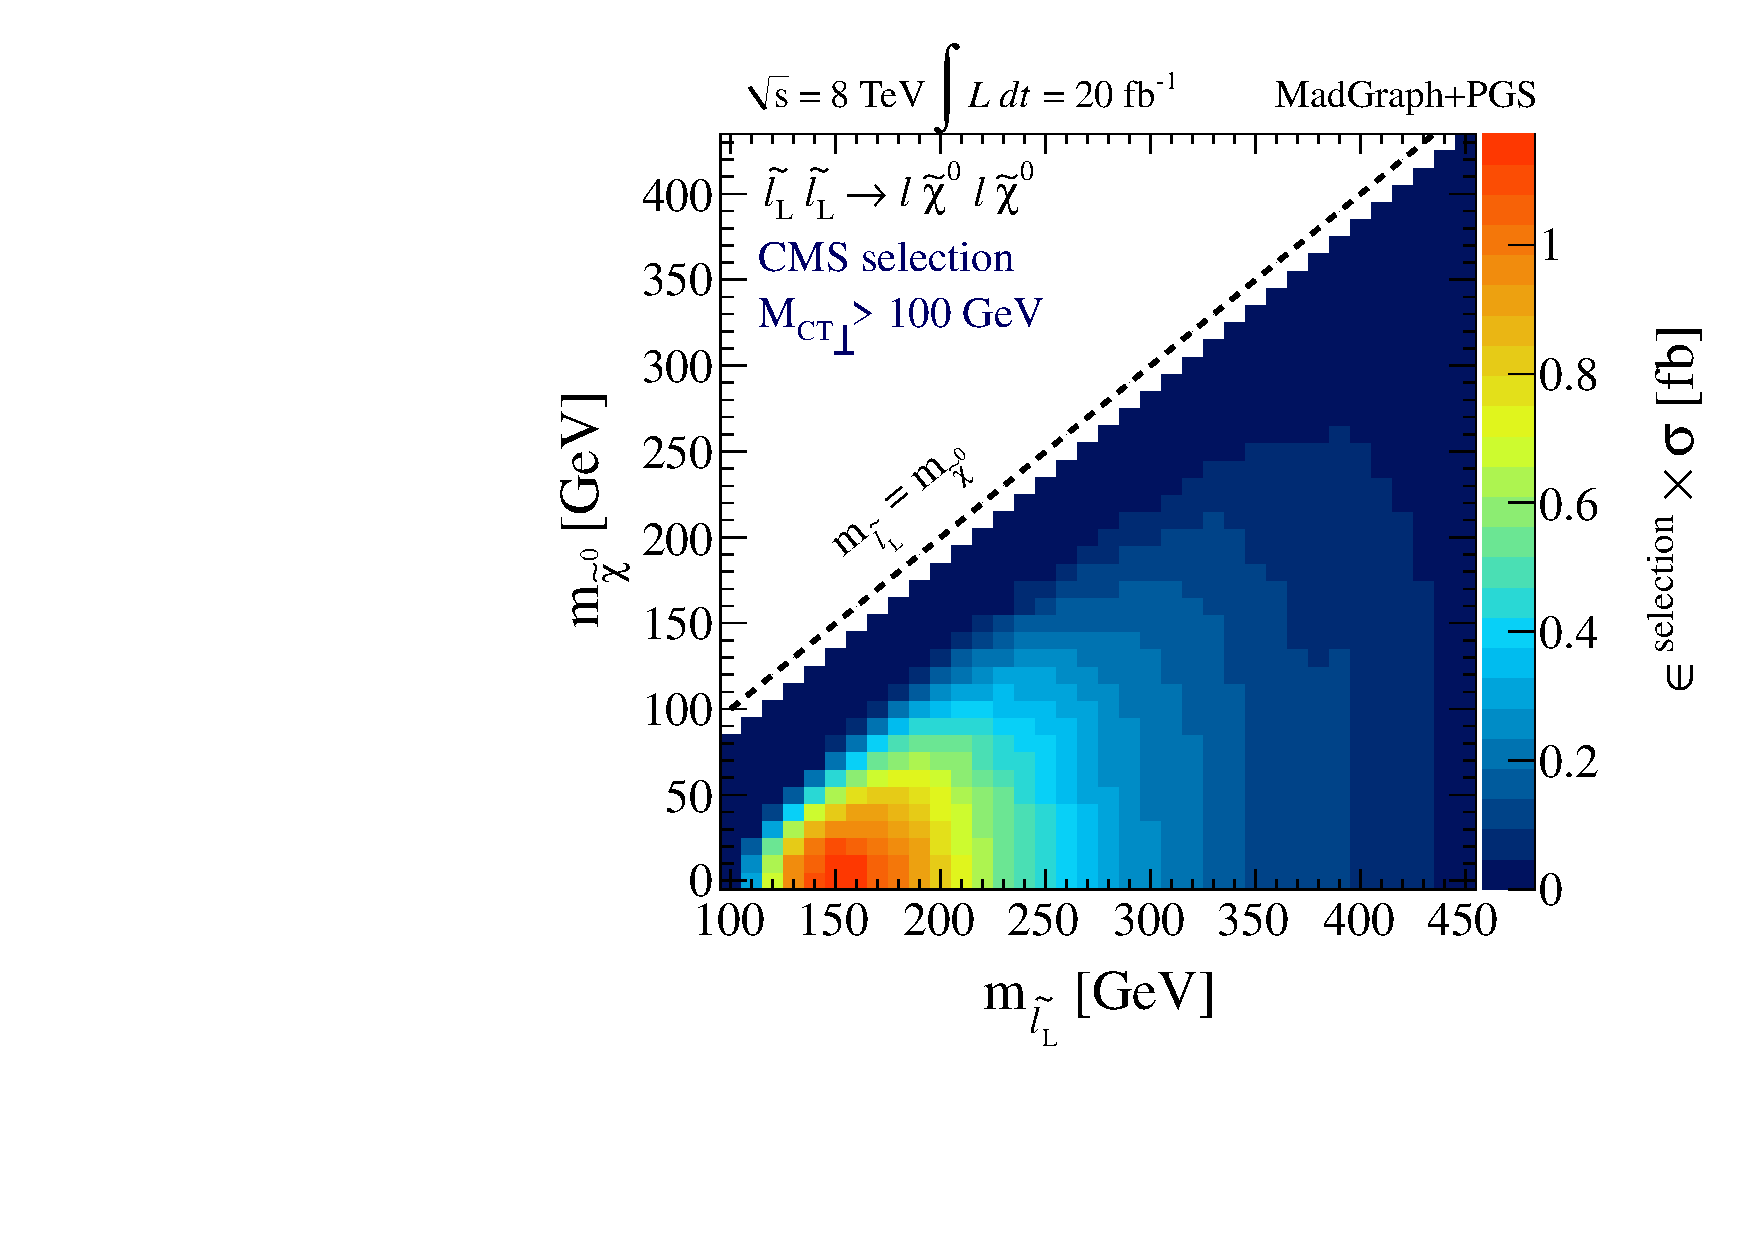
\includegraphics[width=0.35\columnwidth]{fig/sectionIII/XSEC_sleptonL_CMS_MCTperp100.pdf}\\
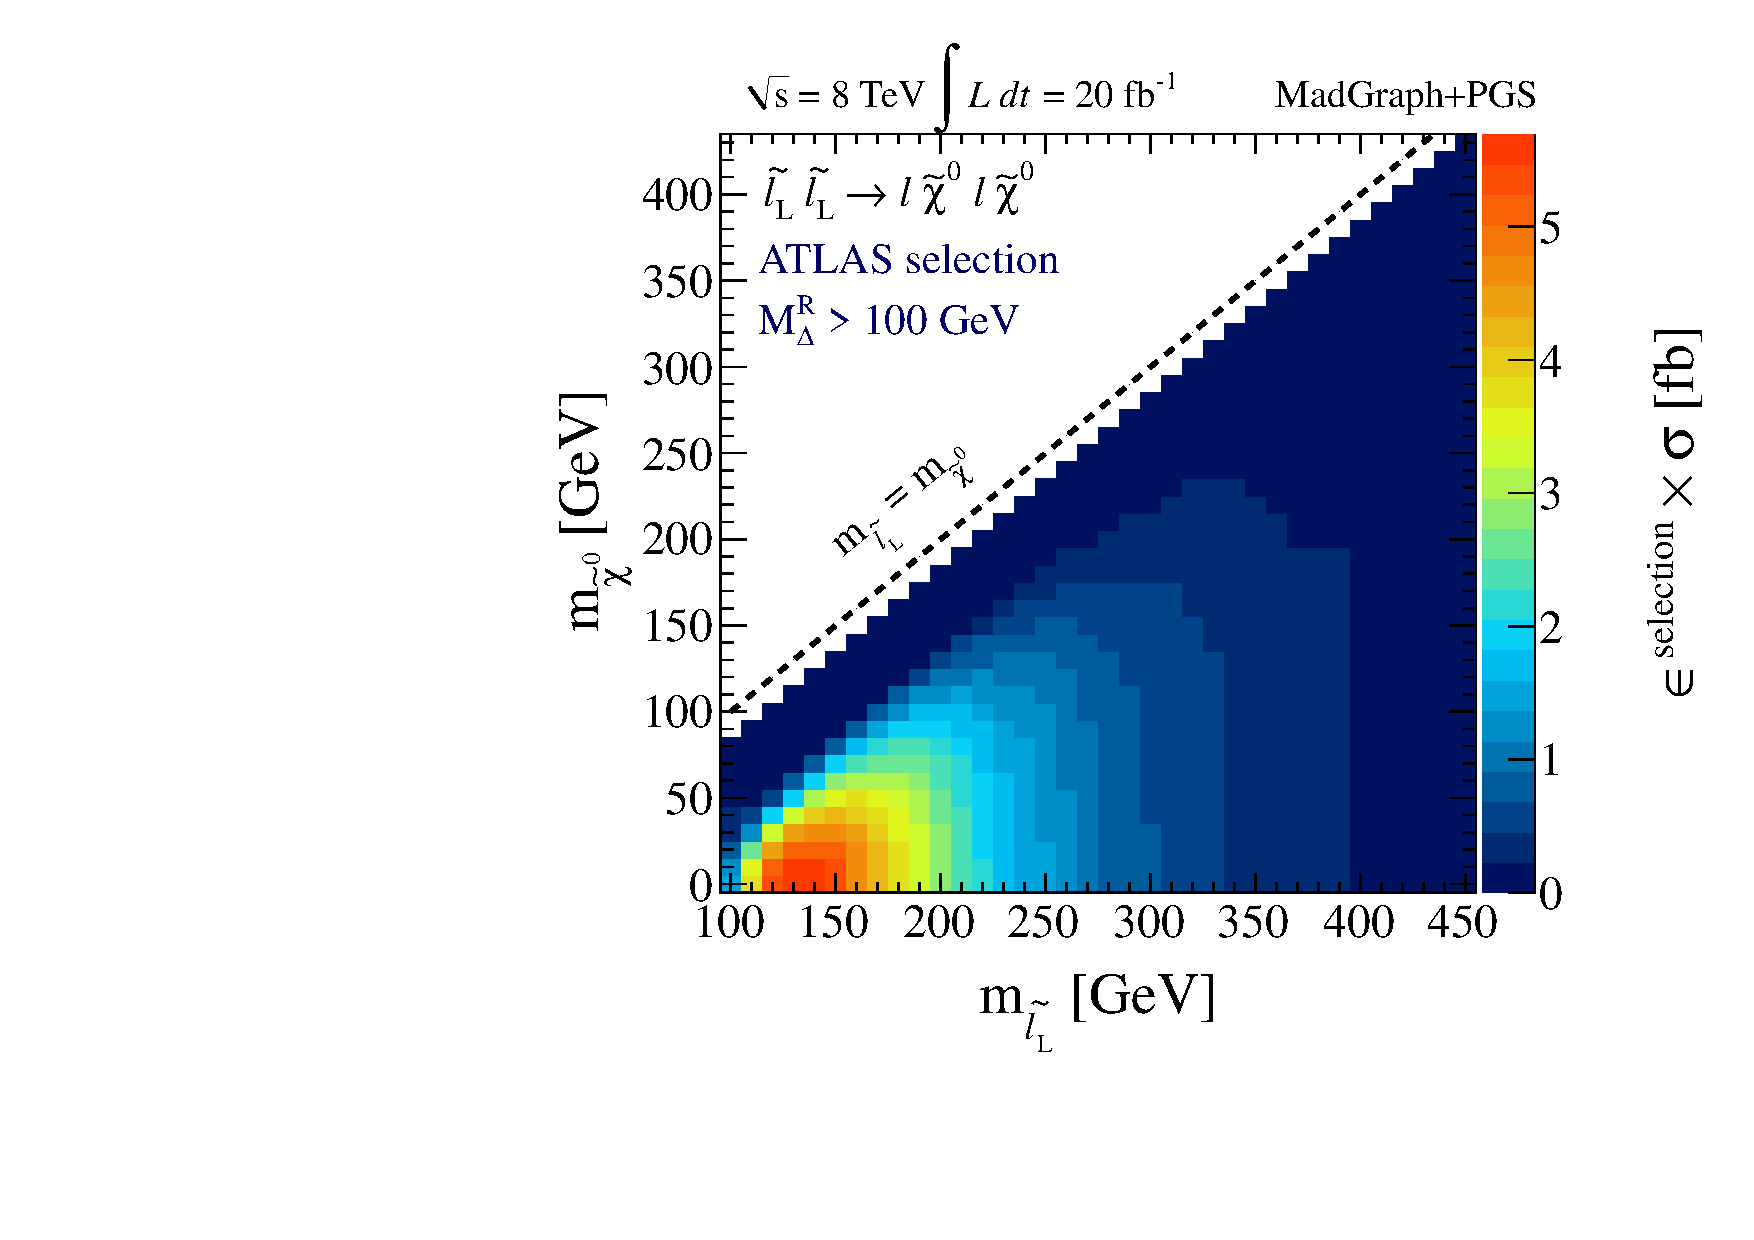
\includegraphics[width=0.35\columnwidth]{fig/sectionIII/XSEC_sleptonL_ATLAS_Mdelta100.pdf}
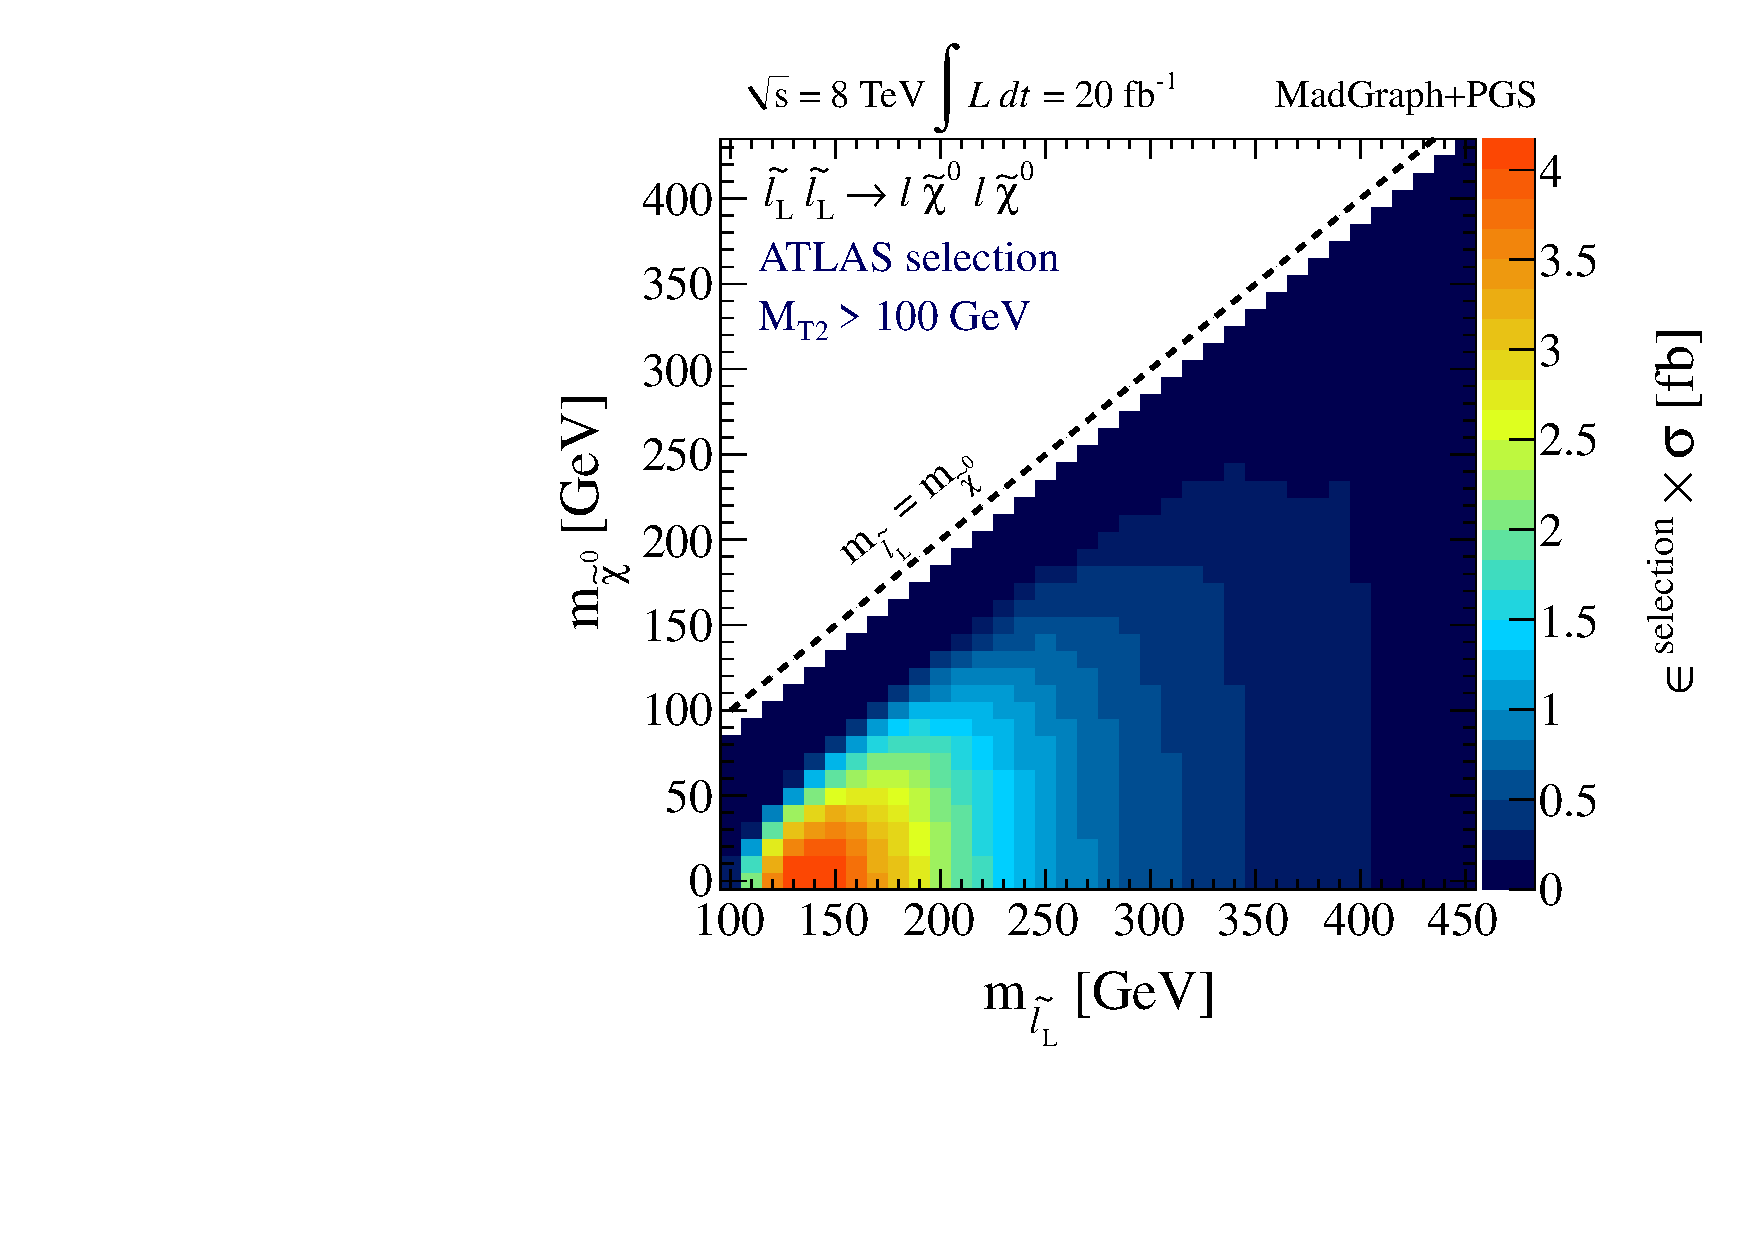
\includegraphics[width=0.35\columnwidth]{fig/sectionIII/XSEC_sleptonL_ATLAS_MT2100.pdf}
\caption{Efficiency times cross section for slepton signal samples, as a function of neutralino mass, for the CMS (top) and ATLAS (bottom) selections with additional requirement that the mass sensitive variable ($M_{\Delta}$ - left, $M_{CT\perp}$ - top right, $M_{T2}$ - bottom right) is in excess of 100~GeV. \label{fig:XSEC_M100_slepton}}
\end{figure}

In practice, the sensitivity of search analyses in this final state will not scale exactly with this inclusive efficiency, due to large differences in background yields as a function of $M_{\Delta}$-sensitive variables. Each of the largest backgrounds after the CMS and ATLAS selections ($WW$ and $t\bar{t}$), have $M_{\Delta}$-sensitive variable distributions that have inherited information of the scale $m_{W}$. Therefore the sensitivity scales strongly with $M_{\Delta}$, with significant experimental reach appearing only once $M_{\Delta}$ is in excess of the $W$ mass. The effective cross-sections for signal models after the additional requirement that the $M_{\Delta}$-sensitive variable used in each analysis is in excess of 100 GeV are shown in Figures~\ref{fig:XSEC_M100_slepton} and~\ref{fig:XSEC_M100_chargino} for sleptons and charginos, respectively. The expected sensitivity of the hypothetical searches described in the following sections closely follows these yields. Efficiencies and cross-sections for the SM backgrounds considered in these analyses are summarized in Table~\ref{tab:BKG}.

\begin{figure}[ht]
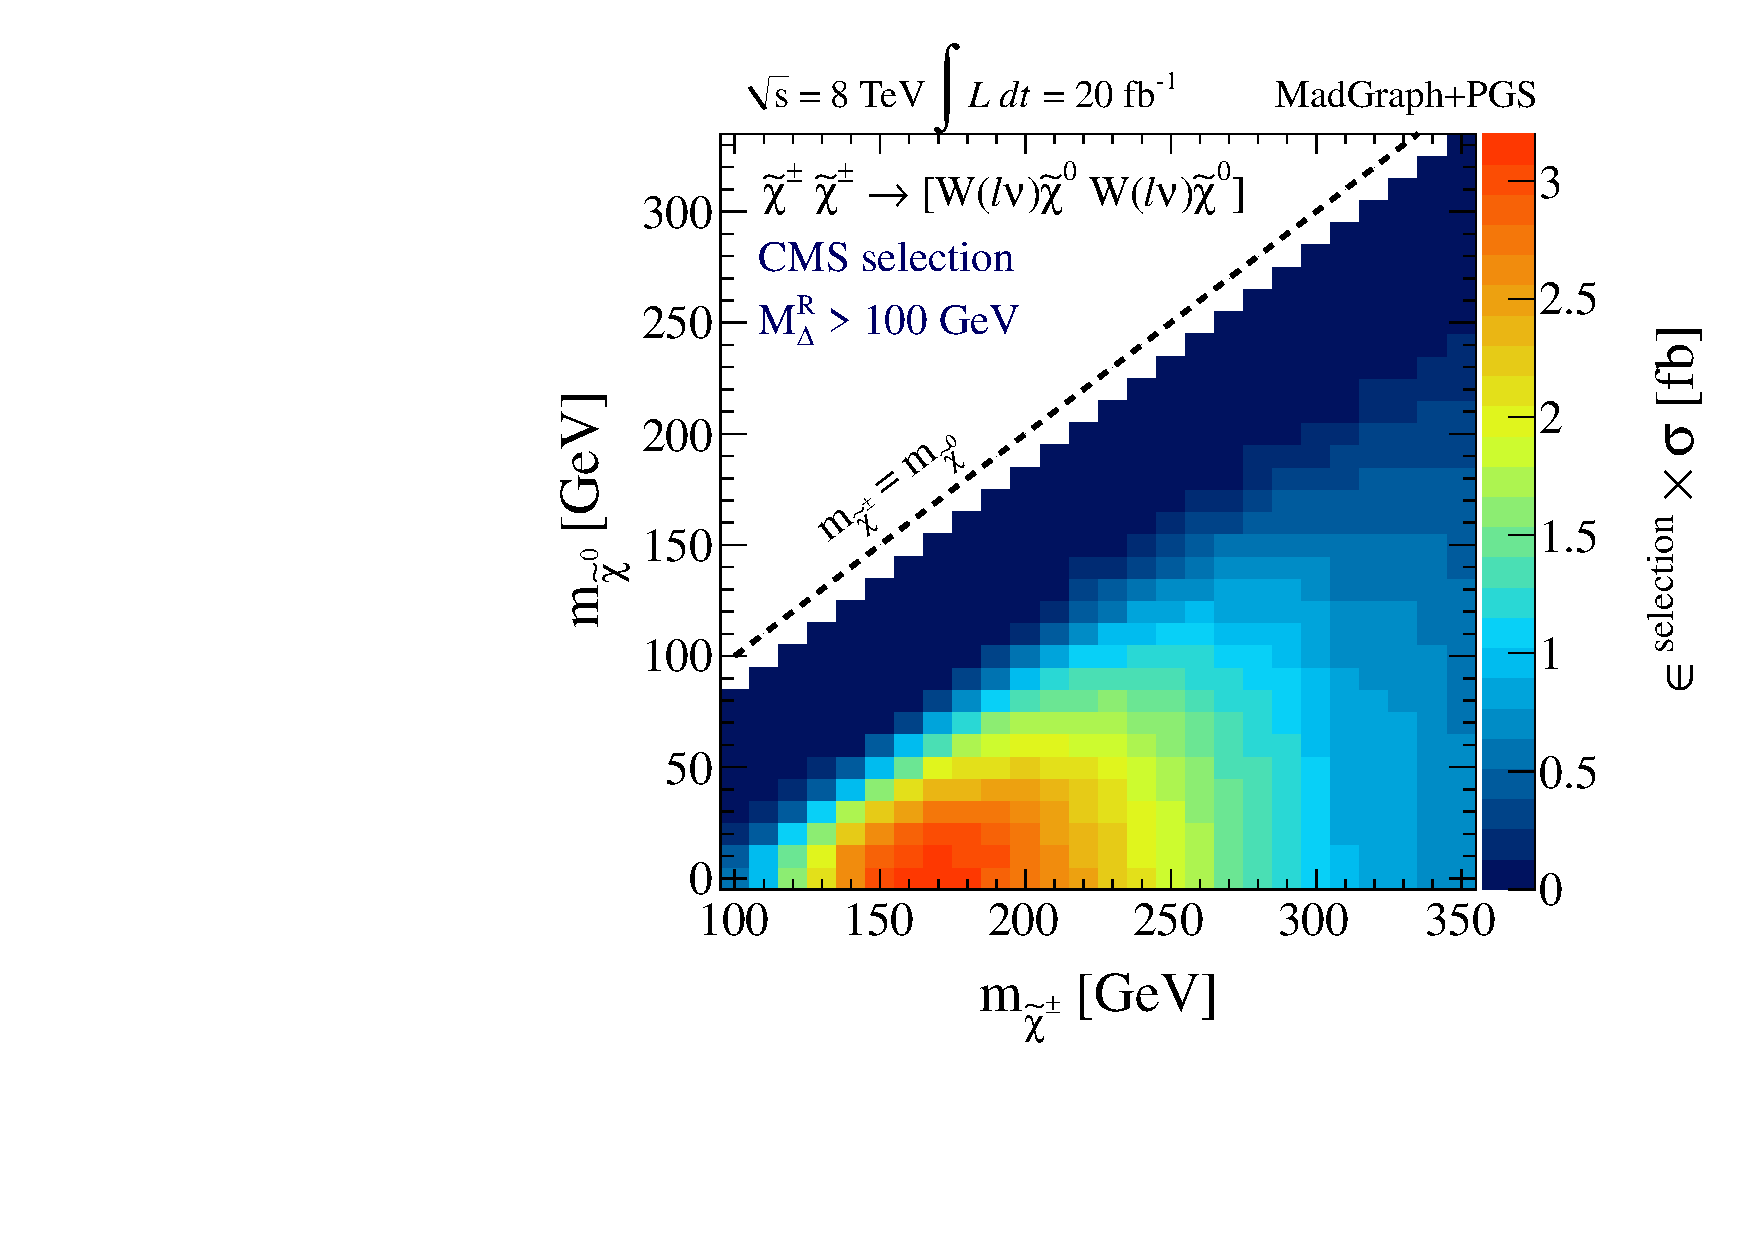
\includegraphics[width=0.35\columnwidth]{fig/sectionIII/XSEC_chargino_CMS_Mdelta100.pdf}
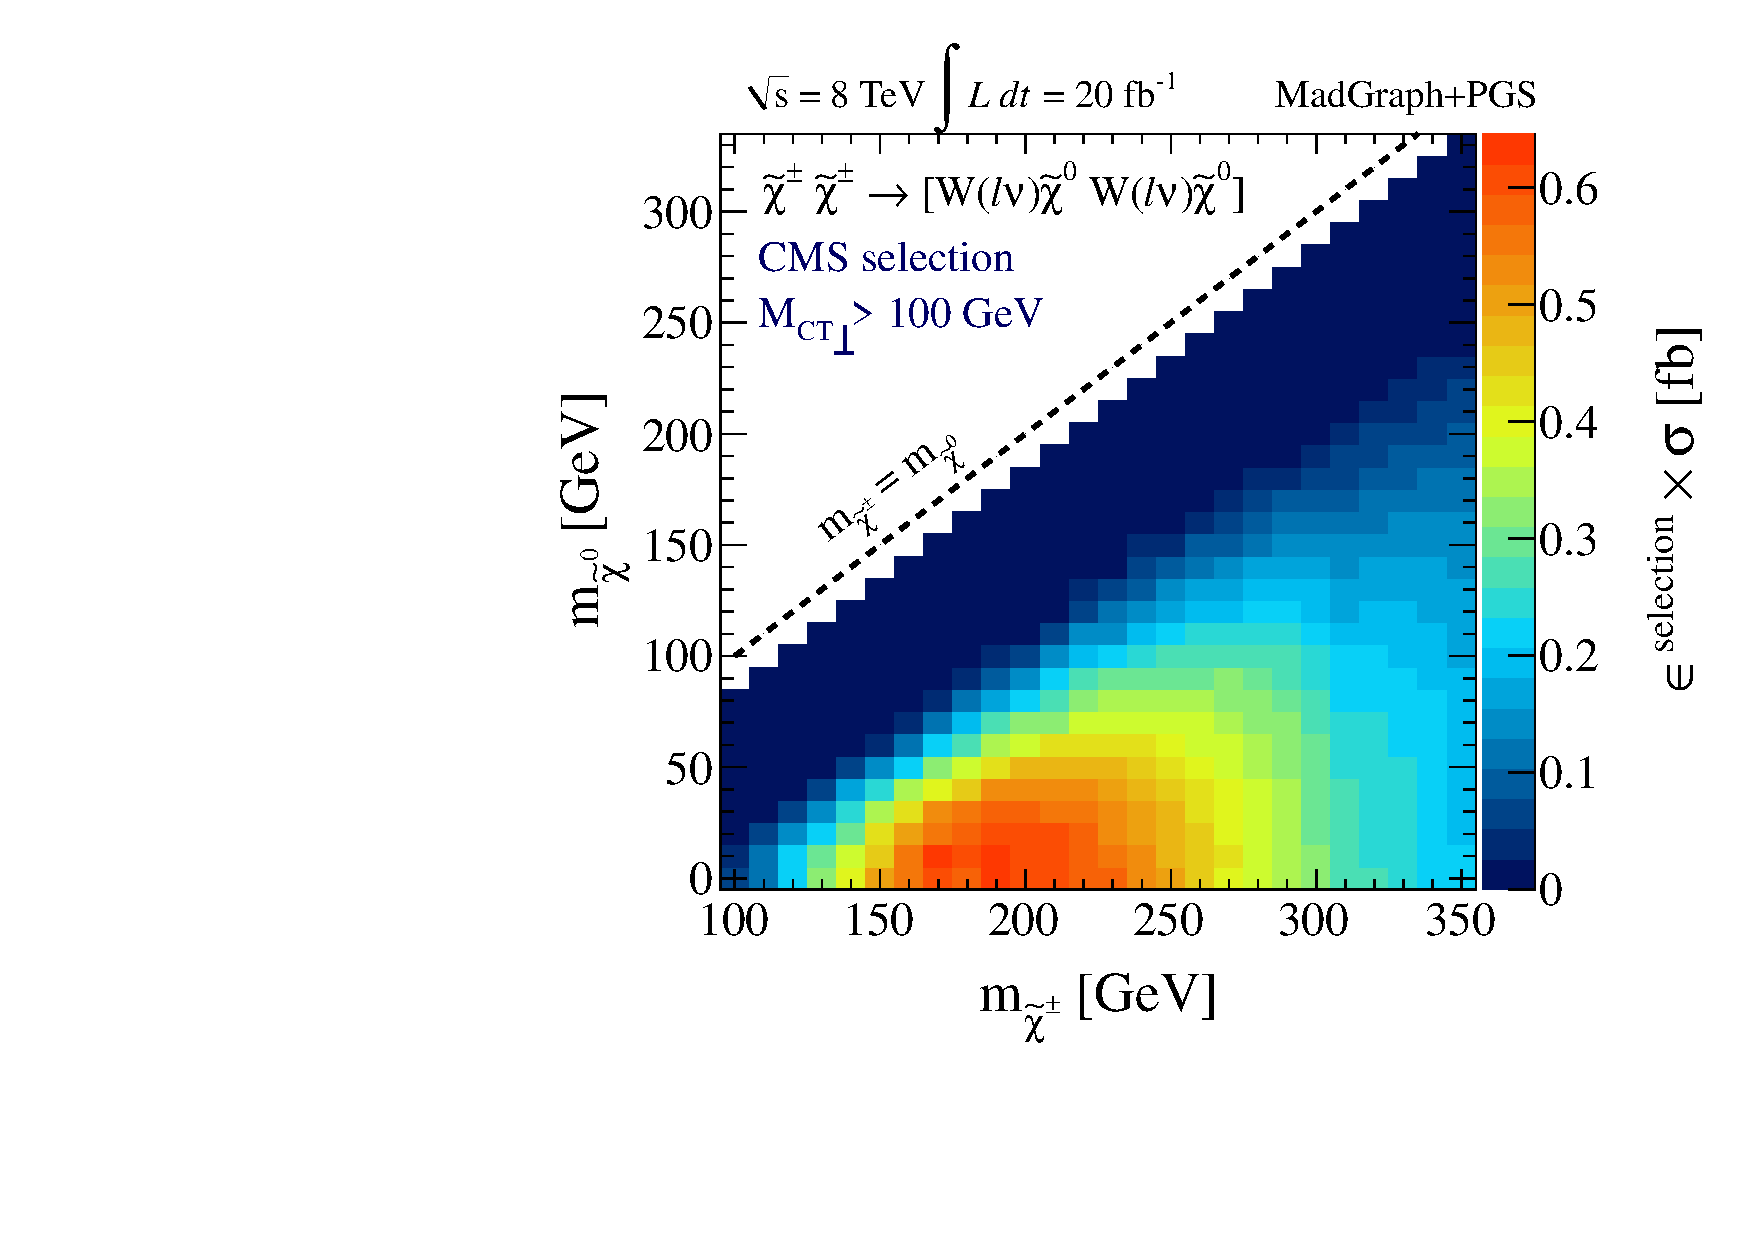
\includegraphics[width=0.35\columnwidth]{fig/sectionIII/XSEC_chargino_CMS_MCTperp100.pdf}\\
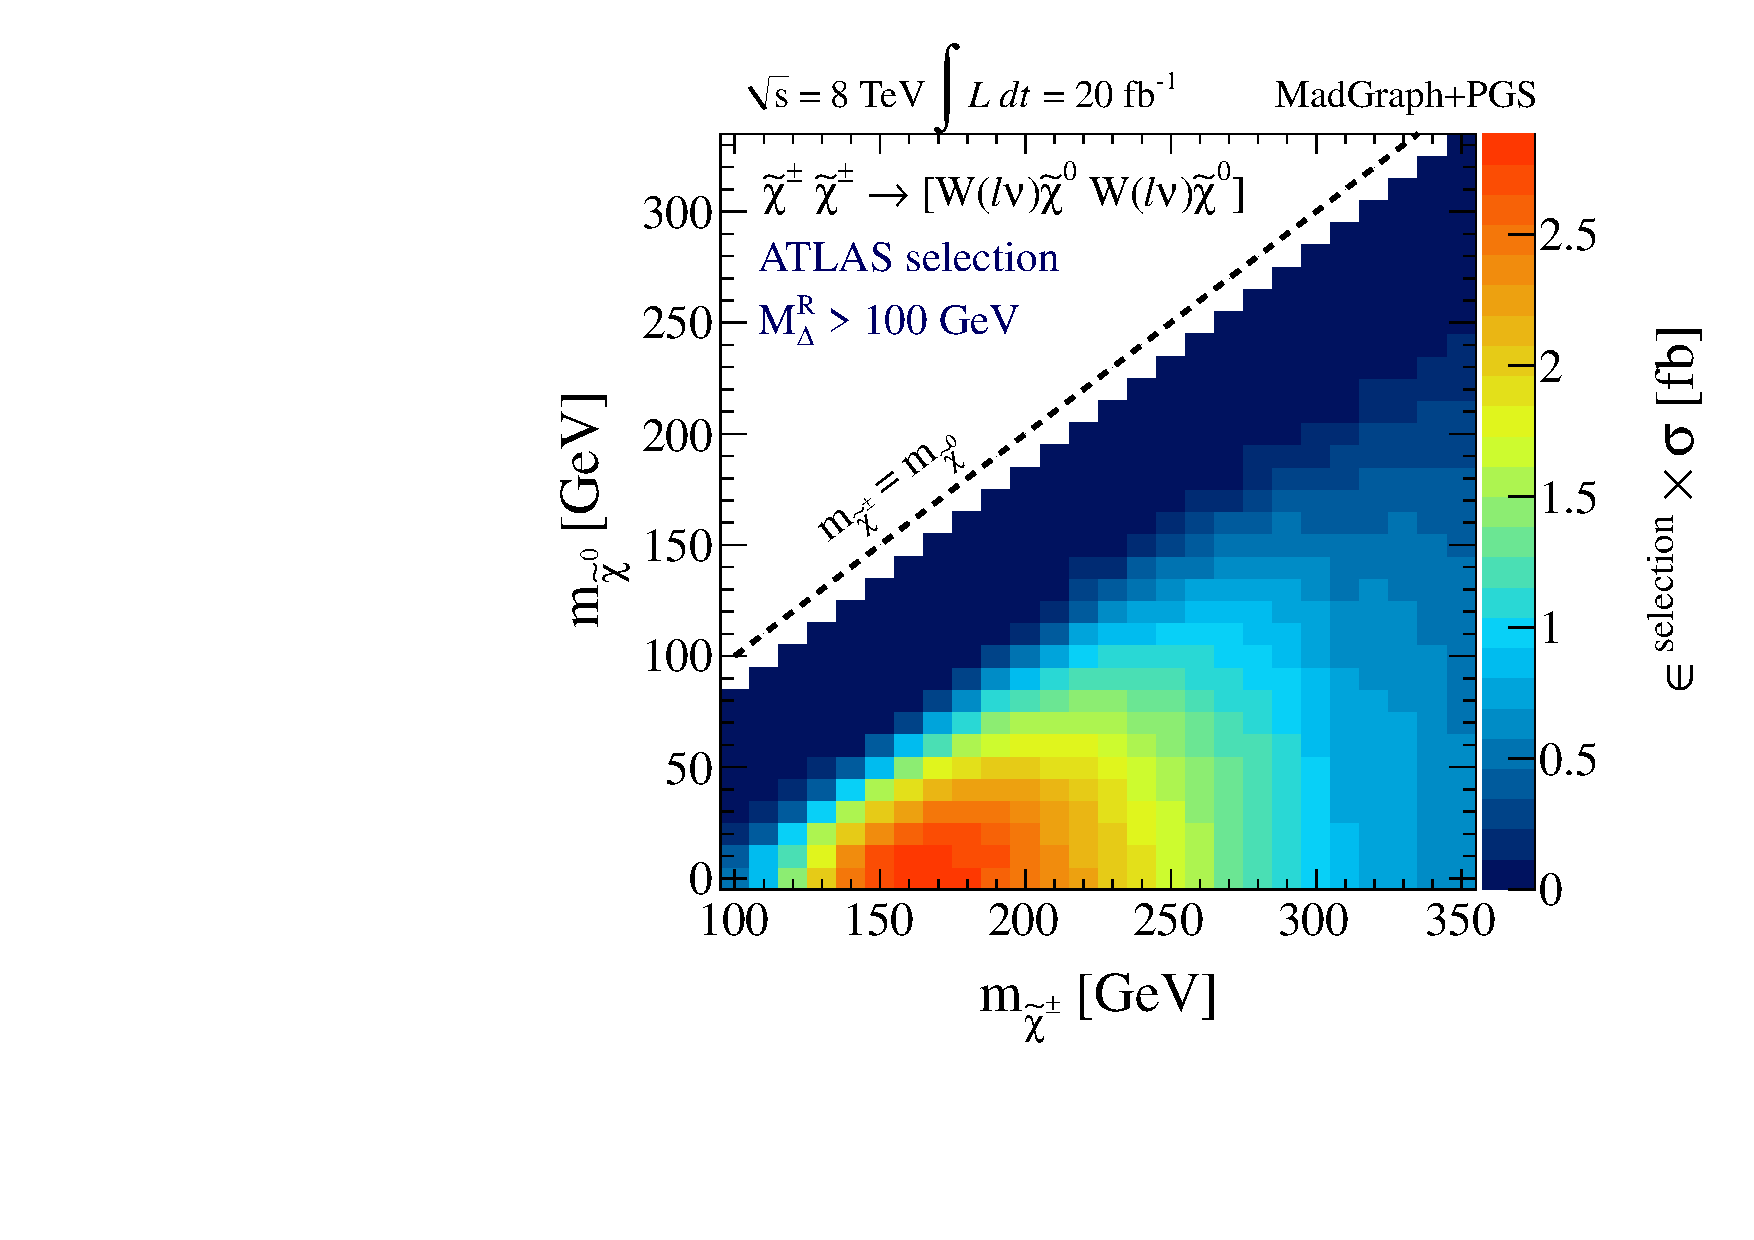
\includegraphics[width=0.35\columnwidth]{fig/sectionIII/XSEC_chargino_ATLAS_Mdelta100.pdf}
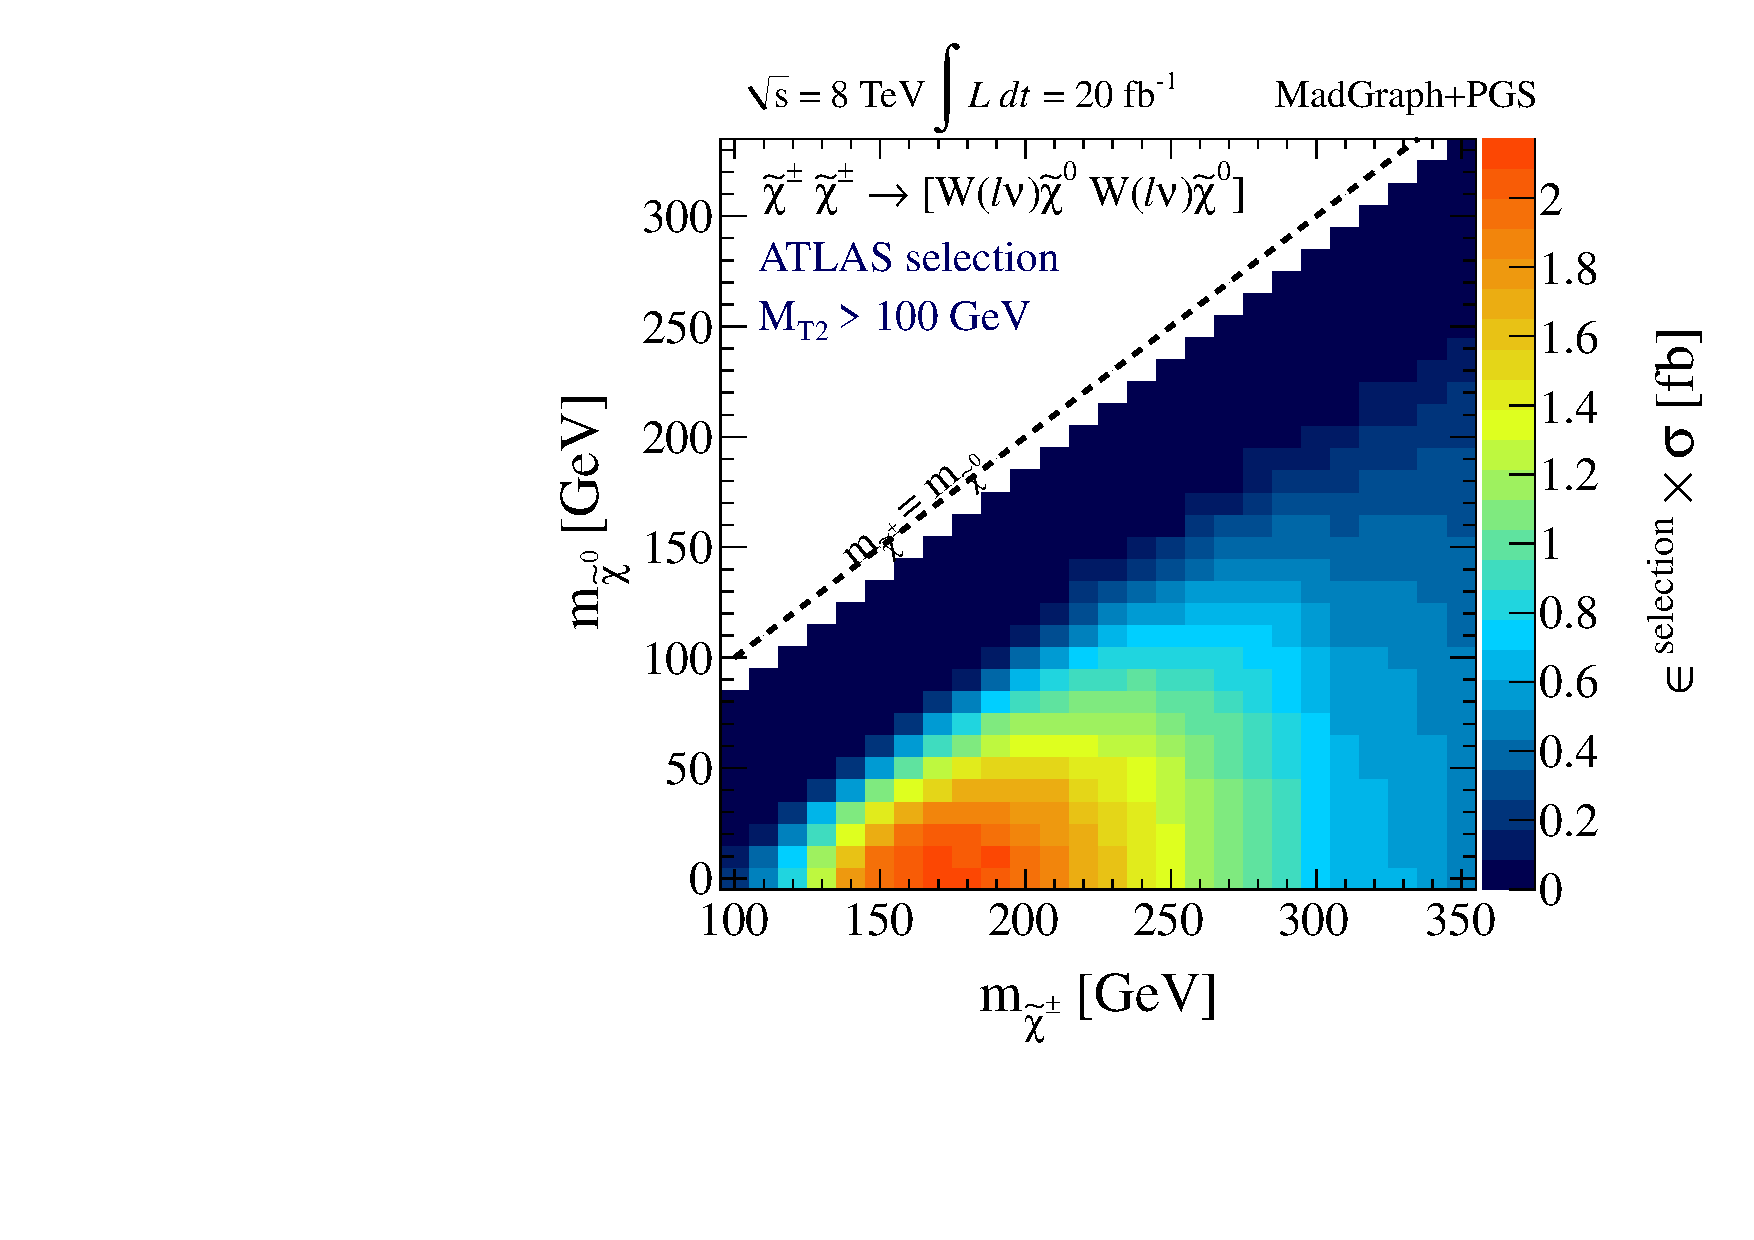
\includegraphics[width=0.35\columnwidth]{fig/sectionIII/XSEC_chargino_ATLAS_MT2100.pdf}
\caption{Efficiency times cross section for chargino signal samples, as a function of neutralino mass, for the CMS (top) and ATLAS (bottom) selections with additional requirement that the mass sensitive variable ($M_{\Delta}$ - left, $M_{CT\perp}$ - top right, $M_{T2}$ - bottom right) is in excess of 100~GeV. \label{fig:XSEC_M100_chargino}}
\end{figure}

\subsection{Super-Razor selection without an $E_{T}^\text{miss}$ cut  }

Kinematic variables sensitive to $M_{\Delta}$ can be powerful discriminants between slepton and chargino signals and SM backgrounds when $M_{\Delta}$ is much larger than the $W$ mass, while heavy sparticle production with relatively compressed spectra can more easily
remain hidden under large SM backgrounds. The angular variables introduced in Section~\ref{sec:variables}, $\Delta \phi_{R}^{\beta}$ and $|\cos\theta_{R+1}|$, are designed to address this deficiency. They are sensitive to quantities in events other than $M_{\Delta}$: the ratio of daughter to parent mass and the spin correlations of decaying particles in the event. Thus they can be used to further discriminate between signal and background. 

Each of the super-razor variables, $M_{\Delta}^{R}$, $\sqrt{\hat{s}}_{R}$, $\vec{\beta}_{R}$, $\vec{\beta}_{R+1}$, $\Delta \phi_{R}^{\beta}$, and $|\cos\theta_{R+1}|$, represents a different piece of information about an event, and the collection can be thought of as a kinematic basis. Here we explore a new kinematic selection based on this basis, attempting to increase sensitivity to models with smaller values of  $M_{\Delta}$. In particular, we consider how one can remove explicit requirements on $E_{T}^\text{miss}$. Included primarily to reject Drell-Yan background, such a requirement is inefficient for signal events at low $M_{\Delta}$. Rather than attempting to determine an optimized set of cuts on the super-razor variables, we demonstrate how a selection criteria can be designed through simple choices for each variable based on the backgrounds we are attempting to reject.

We first consider the triplet of variables $M_{\Delta}^{R}$, $\sqrt{\hat{s}}_{R}$, and $\gamma_{R+1}$, which for di-slepton production are meant to estimate $m_{\tilde{\ell}}$, $\sqrt{\hat{s}}$, and $\gamma^\text{decay}$, respectively. For both the true and reconstructed quantities the three variables represent only two unique pieces of information, since they are related by $\sqrt{\hat{s}}_{R} = 2 \gamma_{R+1}M_{\Delta}^{R}$ and $\sqrt{\hat{s}} = 2 \gamma^\text{decay}m_{\tilde{\ell}}$. Which two variables to consider depends on which signal and backgrounds are being investigated. For example, if searching for $H \to W(\ell\nu)W(\ell\nu)$ the variable $\sqrt{\hat{s}}_{R}$ will be resonant at the Higgs mass. If the Higgs is too light to accommodate two on-shell $W$'s then the variables  $M_{\Delta}^{R}$ and $\gamma_{R+1}$ are more difficult to interpret, representing a combination of two $W$ bosons with different masses. For the case of interest in this paper, non-resonant slepton pair production, off-shell sleptons are kinematically suppressed, and so  $M_{\Delta}^{R}$, $\sqrt{\hat{s}}_{R}$ and $\gamma_{R+1}$ are all meaningful. However, they are not equally useful for discriminating between signal and background.
 
For di-slepton pair production the quantity that $M_{\Delta}^{R}$ is attempting to measure is effectively constant event by event, and is useful for discriminating against backgrounds.  On the other hand, $\gamma^\text{decay}$ varies between events, characteristic of non-resonant production, as does  $WW$ and $t\bar{t}$ backgrounds. As a result, $\sqrt{\hat{s}}_{R}$ provides information largely redundant with $M_{\Delta}^{R}$ while $\gamma_{R+1}$ does not strongly discriminate against these large backgrounds. 

\begin{figure}[ht]
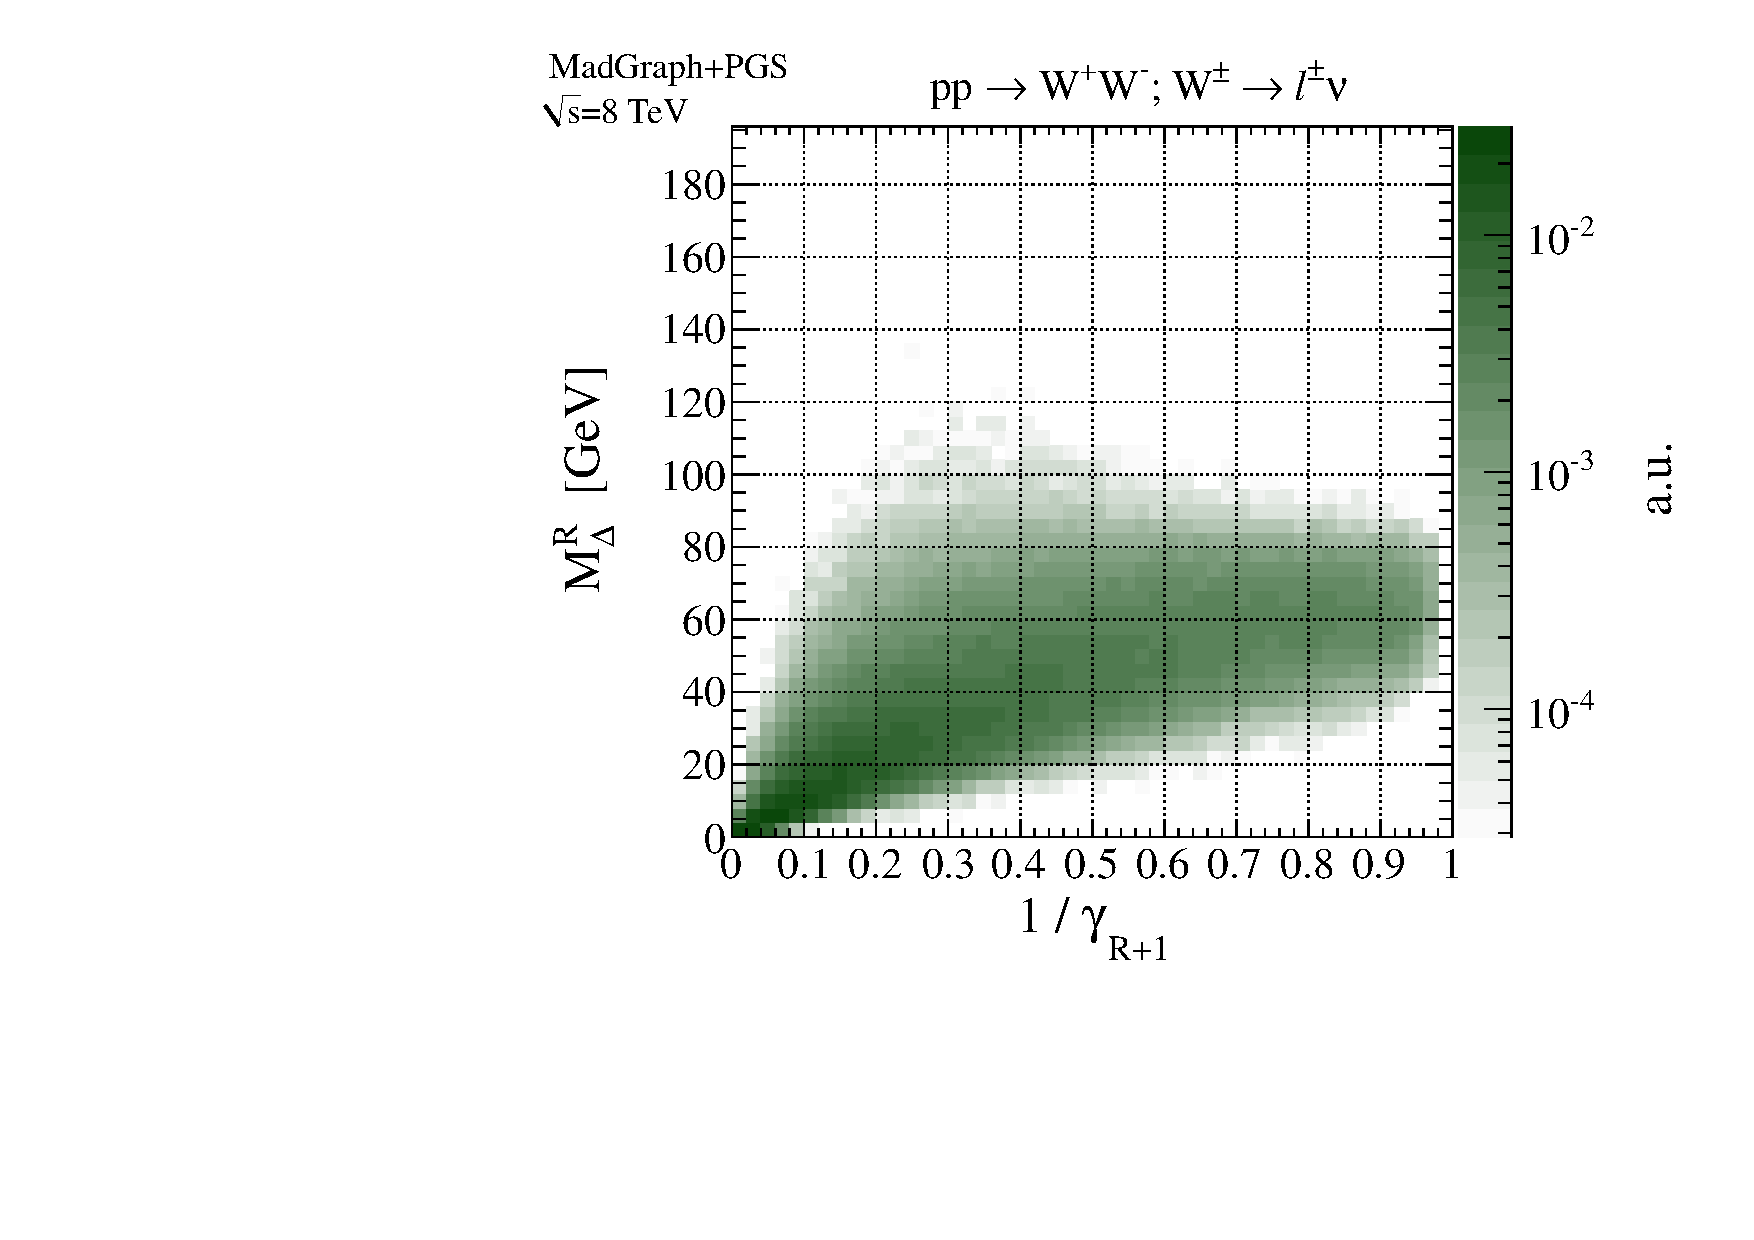
\includegraphics[width=0.3\columnwidth]{fig/sectionIII/Mdelta_v_gamma_WW.pdf}
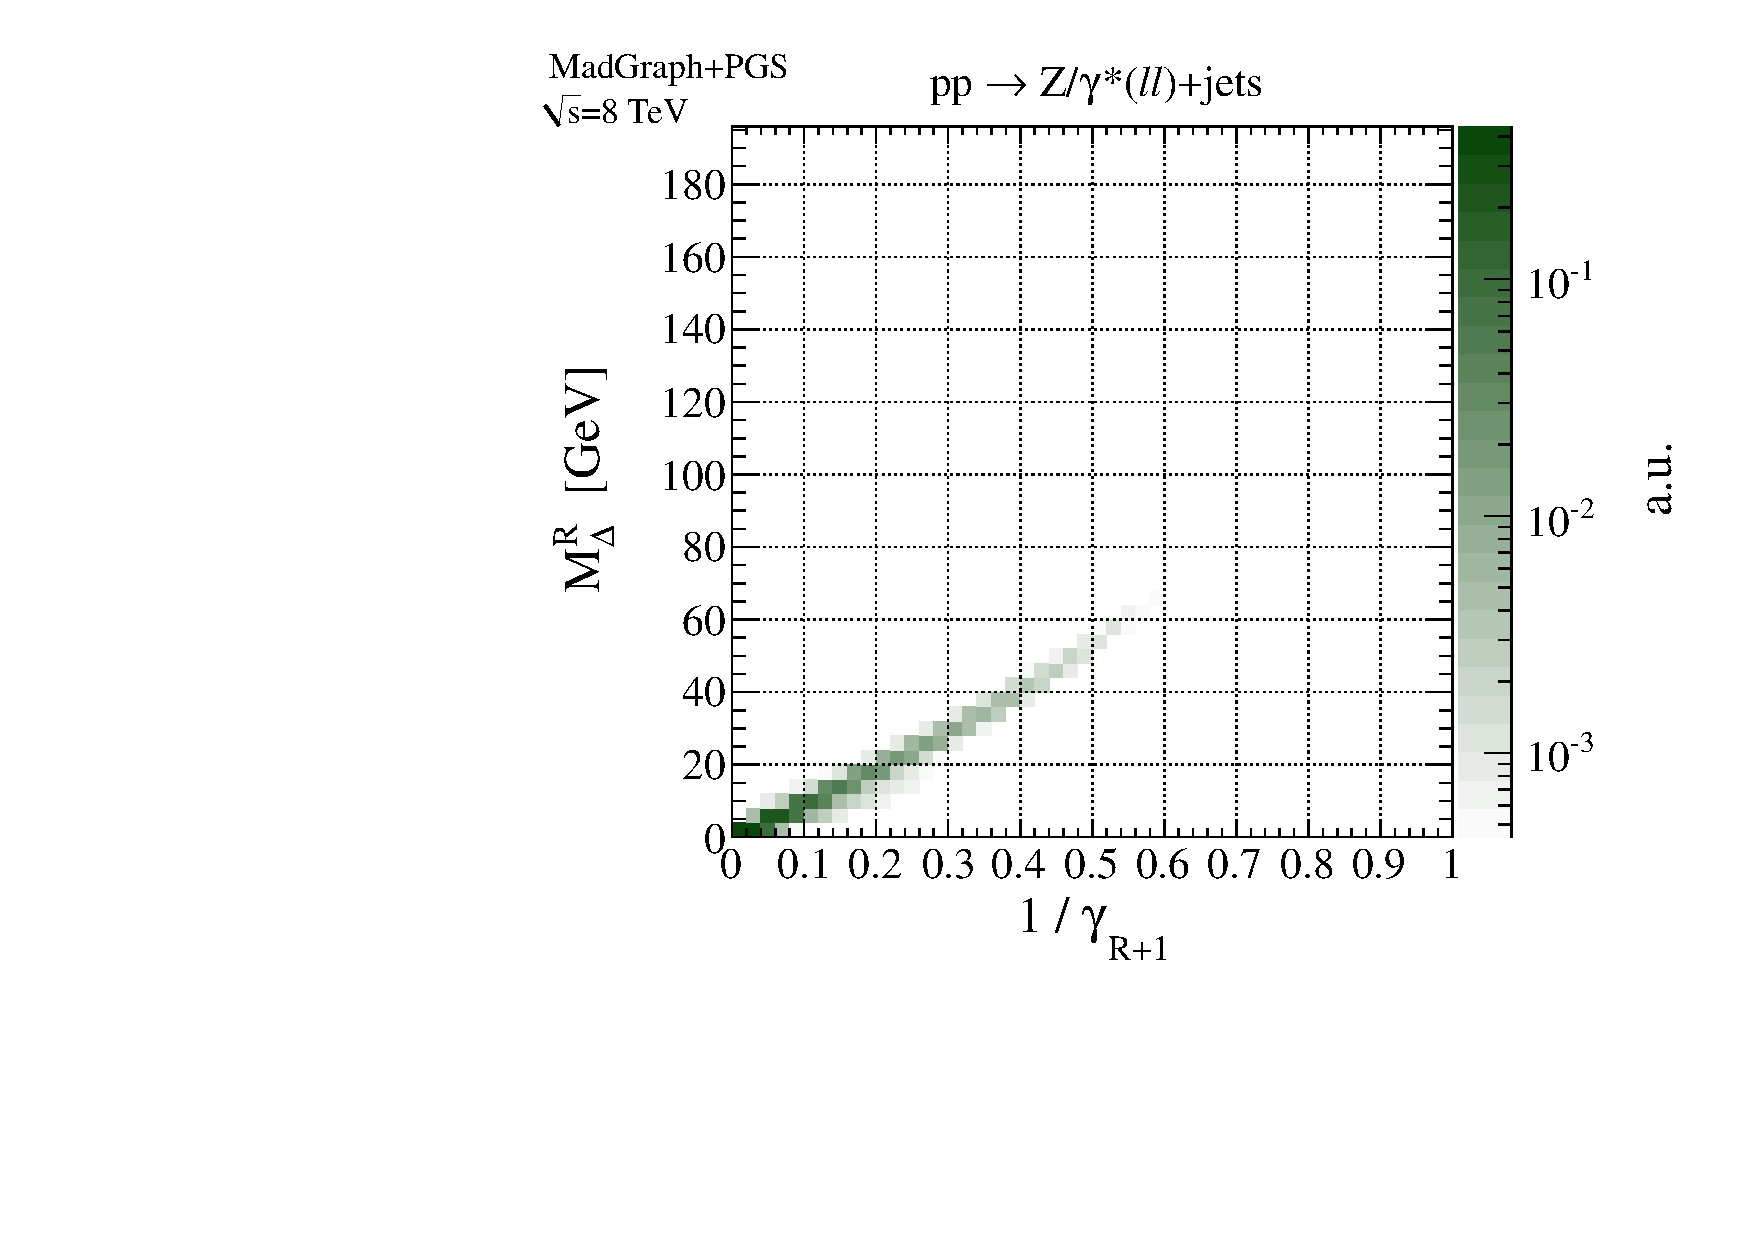
\includegraphics[width=0.3\columnwidth]{fig/sectionIII/Mdelta_v_gamma_DY.pdf} \\
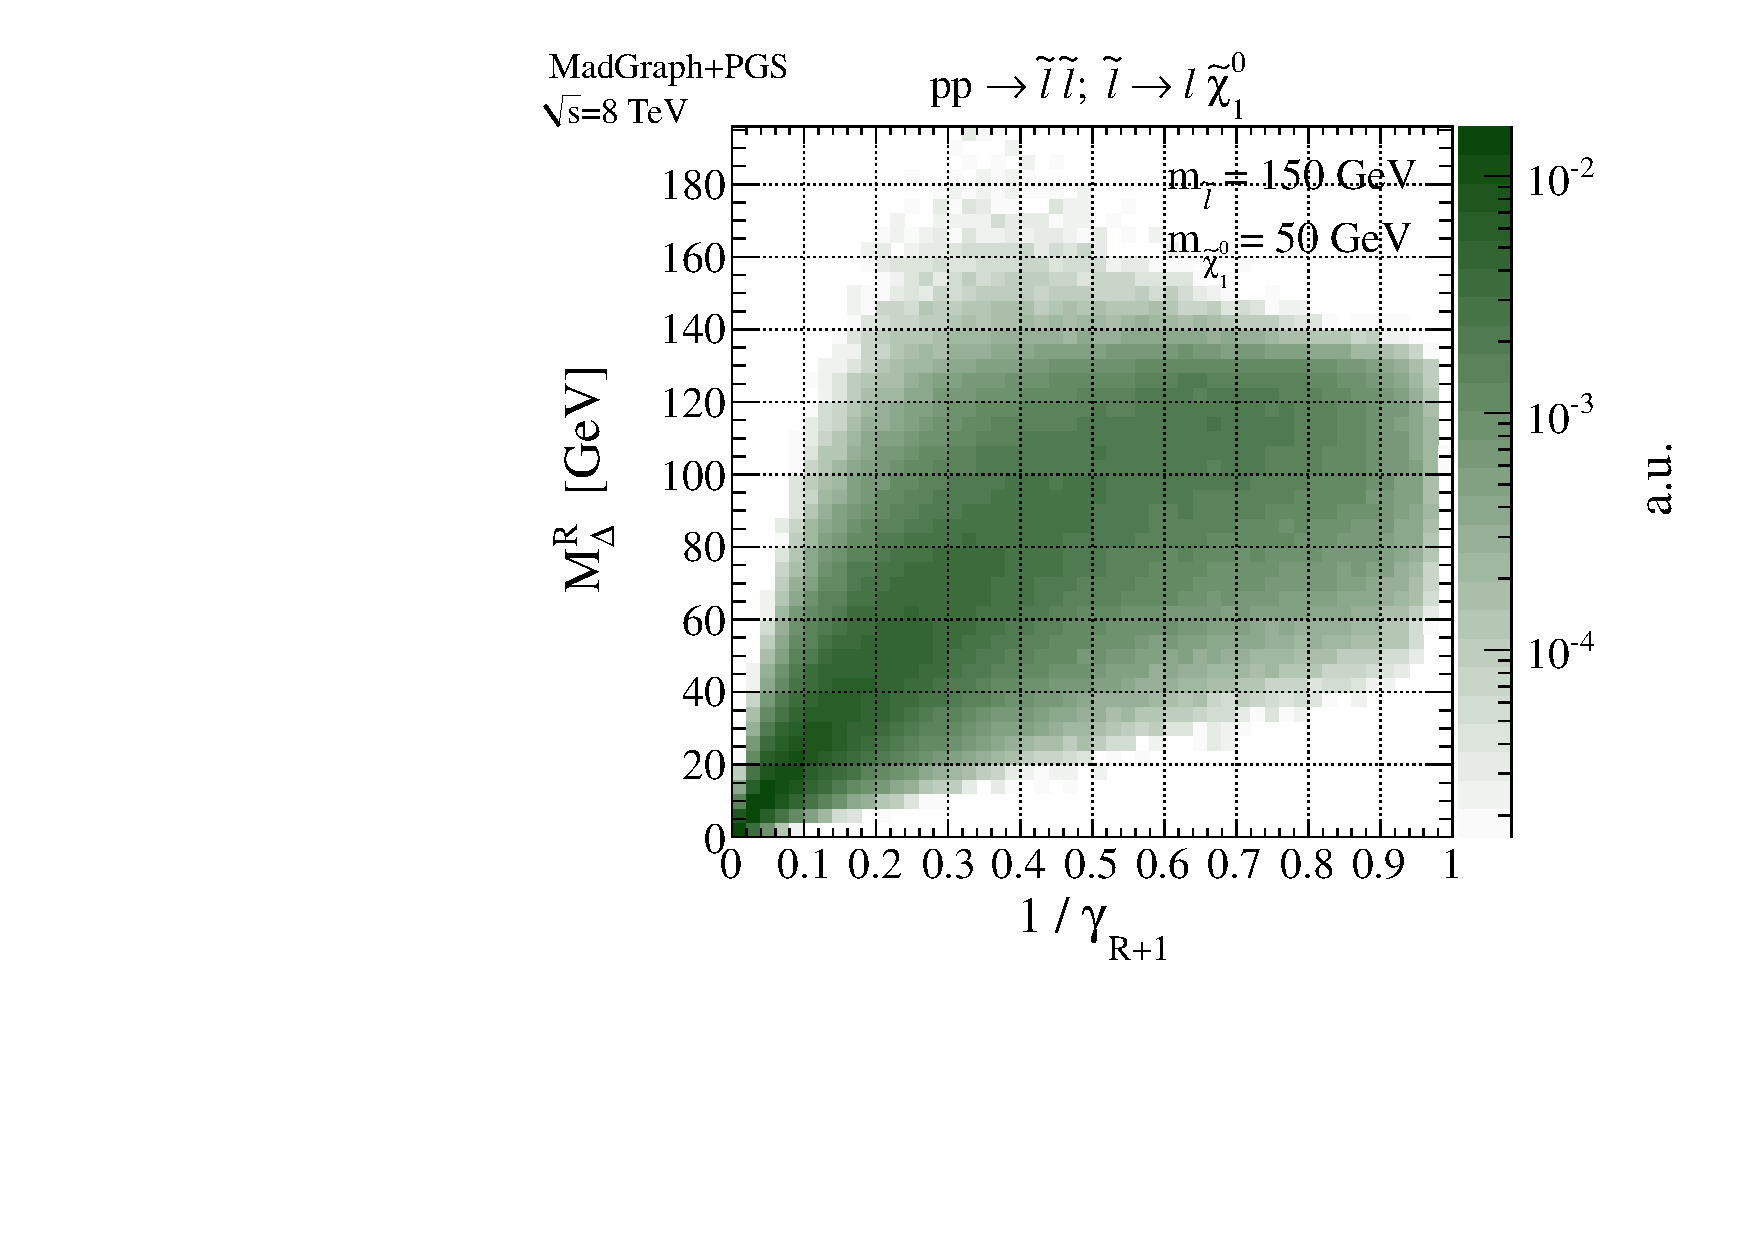
\includegraphics[width=0.3\columnwidth]{fig/sectionIII/Mdelta_v_gamma_slepton_150_50.pdf}
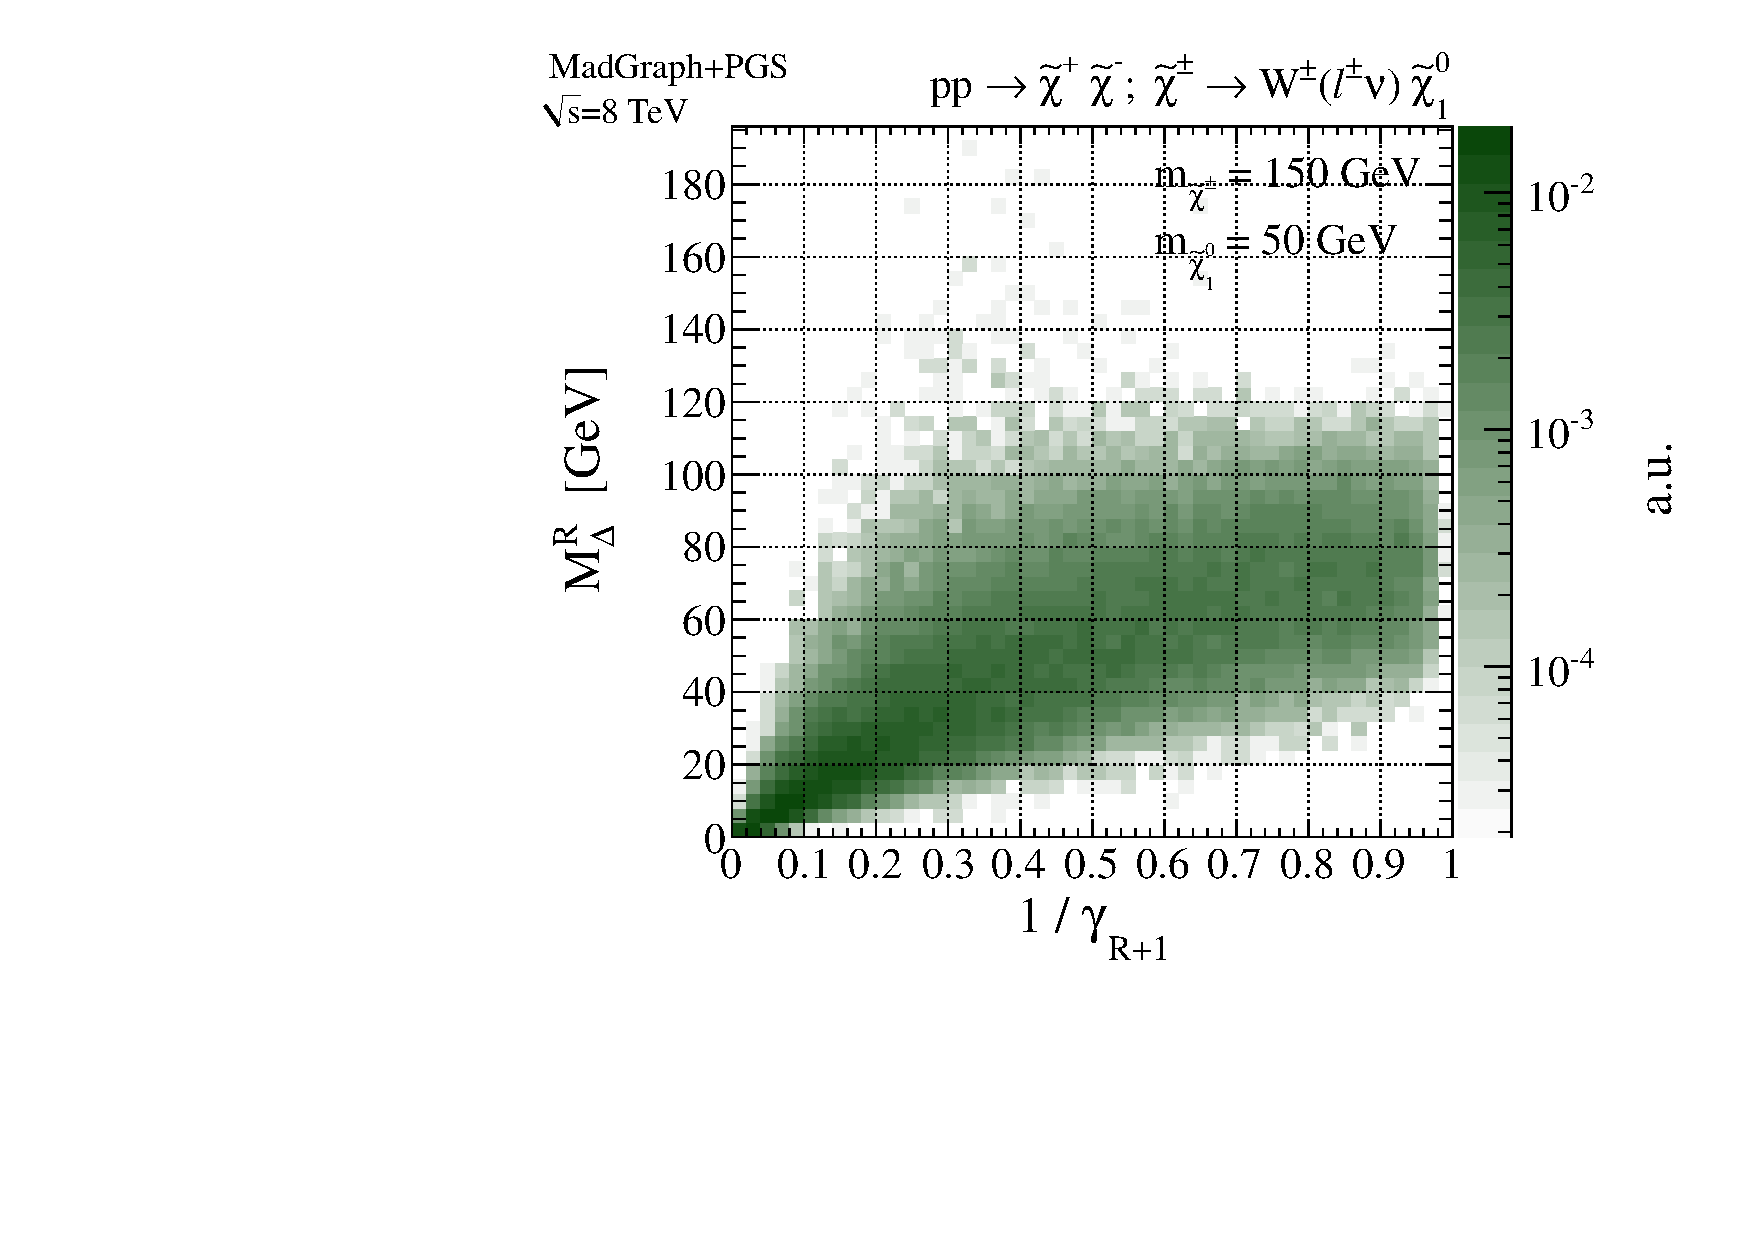
\includegraphics[width=0.3\columnwidth]{fig/sectionIII/Mdelta_v_gamma_chargino_150_50.pdf}
\caption{Distributions of $M_{\Delta}^{R}$ vs. $1/\gamma_{R+1}$ for simulated events samples with baseline selection applied. Top left: $WW$. Top right: $Z/\gamma*$+jets. Bottom left: di-slepton production with $m_{\tilde{\ell}} = 150$~GeV and  $m_{\tilde{\chi}^0_1} = 50$~GeV. Bottom right: di-chargino production with $m_{\tilde{\chi}^{\pm}_{1}} = 150$~GeV and  $m_{\tilde{\chi}^0_1} = 50$~GeV. \label{fig:Mdelta_v_gamma}}
\end{figure}

The distributions of $M_{\Delta}^{R}$ as a function of $1/\gamma_{R+1}$, for simulated signal and background events, are shown in Figure~\ref{fig:Mdelta_v_gamma}. We observe that, for large $1/\gamma_{R+1}$, the two variables are largely uncorrelated for signal events. For small values of this variable, the signal $M_{\Delta}^{R}$ distribution collapses to zero, corresponding to the case where $\gamma^\text{decay}$ is large and the decay leptons are largely back-to-back in the CM frame. For backgrounds, smaller values of $1/\gamma_{R+1}$ correspond to larger $M_{\Delta}^{R}$ on average. This is especially true for $Z/\gamma^{*}$+jets events; fixed di-lepton invariant mass corresponds to positively correlated lines in the $M_{\Delta}^{R}$ versus $1/\gamma_{R+1}$ plane, as seen in Figure~\ref{fig:Mdelta_v_gamma}. We observe that requiring $1/\gamma_{R+1}$ to be above some small value can remove many background events, especially $Z/\gamma^{*}$+jets, while only removing signal events that fall in an unremarkable region of phase-space (away from their $M_{\Delta}^{R}$ edge).

Resonant di-lepton production from $Z/\gamma^{*}$+jets is a particularly pernicious background. Associated jets produced in the event can boost the di-leptons to topologies that mimic those of di-slepton signals. Spurious $E_{T}^\text{miss}$, often from mis-measurements of jets, prevents this effect from being correctly accounted for. While an absolute requirement on $E_{T}^\text{miss}$ can be used to remove many of these events, this also sets a lower bound $M_{\Delta}$ to which an analysis will be sensitive. Furthermore, $Z/\gamma^{*}$+jets with large $E_{T}^\text{miss}$ that survive such a cut will tend to have large $M_{\Delta}^{R}$, appearing in the region of phase-space we had hoped to query for signal events. To replace a $E_{T}^\text{miss}$ cut, we consider cuts based on scale-less variables, such that background events looking most like signal are also removed and we retain sensitivity to lower values of $M_{\Delta}^{R}$.

The variable $\vec{\beta}_{R}$ is highly sensitive to the mis-measurements which make $Z/\gamma^{*}$+jets a difficult background to remove with $E_T^\text{miss}$ cuts. This boost approximates the transverse portion of the Lorentz transformation from the lab frame to CM frame. Mis-calculations in the reconstruction of the direction and magnitude of this boost leave di-leptons from $Z/\gamma^{*}$ decays in imbalanced configurations while they would be back-to-back in their true CM frame. The magnitude of $\vec{\beta}_{R}$ is not a strong discriminant (it is related to the ratio of CM system $p_{T}$ and its reconstructed mass) while its direction is used in the calculation of $\Delta \phi_{R}^{\beta}$, as discussed in Section~\ref{sec:variables}. 

Another angle that is useful to consider in diagnosing mis-measured $Z/\gamma^{*}$+jets events is the azimuthal angle between the $E_{T}^\text{miss}$ and di-lepton system in the lab frame, $|\Delta\phi (\vec{p}_{\ell\ell}^{\, \text{lab}},\vec{E}_{T}^\text{miss})|$, in particular for its correlation with $\Delta \phi_{R}^{\beta}$. The distribution of $|\Delta\phi (\vec{p}_{\ell\ell}^{\, \text{lab}},\vec{E}_{T}^\text{miss})|$ is shown as a function of $\Delta \phi_{R}^{\beta}$ in Figure~\ref{fig:dphi_v_dphi}. For signal events the distribution of $|\Delta\phi (\vec{p}_{\ell\ell}^{\, \text{lab}},\vec{E}_{T}^\text{miss})|$ is concentrated at $\pi$; the weakly interacting and di-lepton systems are back-to-back in the CM frame and will remain so in the lab frame without a large CM system transverse momentum. The distribution is more dispersed for $t\bar{t}$ events, as the $W$ bosons are not only recoiling against each other in the CM frame, but also against two $b$-quarks. For $Z/\gamma^{*}$+jets the direction of the $\vec{E}_{T}^\text{miss}$ is largely uncorrelated with the di-lepton system. The strength of the information contained in this two-dimensional plane can be seen when considering only events with $\gamma_{R+1} < 4$, {\it i.e.}~those events which tend towards larger $M_{\Delta}^{R}$ values and are therefore of more significance in an analysis. We observe in the bottom part of Figure~\ref{fig:dphi_v_dphi} that while the di-slepton and $t\bar{t}$ samples retain a similar shape after the $\gamma_{R+1} < 4$ requirement, the remaining $Z/\gamma^{*}$+jets exhibit a very particular correlation between $|\Delta\phi (\vec{p}_{\ell\ell}^{\, \text{lab}},\vec{E}_{T}^\text{miss})|$ and $\Delta\phi_{R}^{\beta}$. The most difficult $Z/\gamma^{*}$+jets events, while still having a relatively flat $|\Delta\phi (\vec{p}_{\ell\ell}^{\, \text{lab}},\vec{E}_{T}^\text{miss})|$ distribution tend to gather at low $\Delta \phi_{R}^{\beta}$. The correlation is such that a cut of $\Delta\phi_{R}^{\beta} + |\Delta\phi (\vec{p}_{\ell\ell}^{\, \text{lab}},\vec{E}_{T}^\text{miss})| > \pi$ removes the majority of $Z/\gamma^{*}$+jets while keeping almost all the significant di-slepton events. This cut is indicated by the dotted red line in the bottom part of Figure~\ref{fig:dphi_v_dphi}, events being rejected if they fall below it.

\begin{figure}[ht]
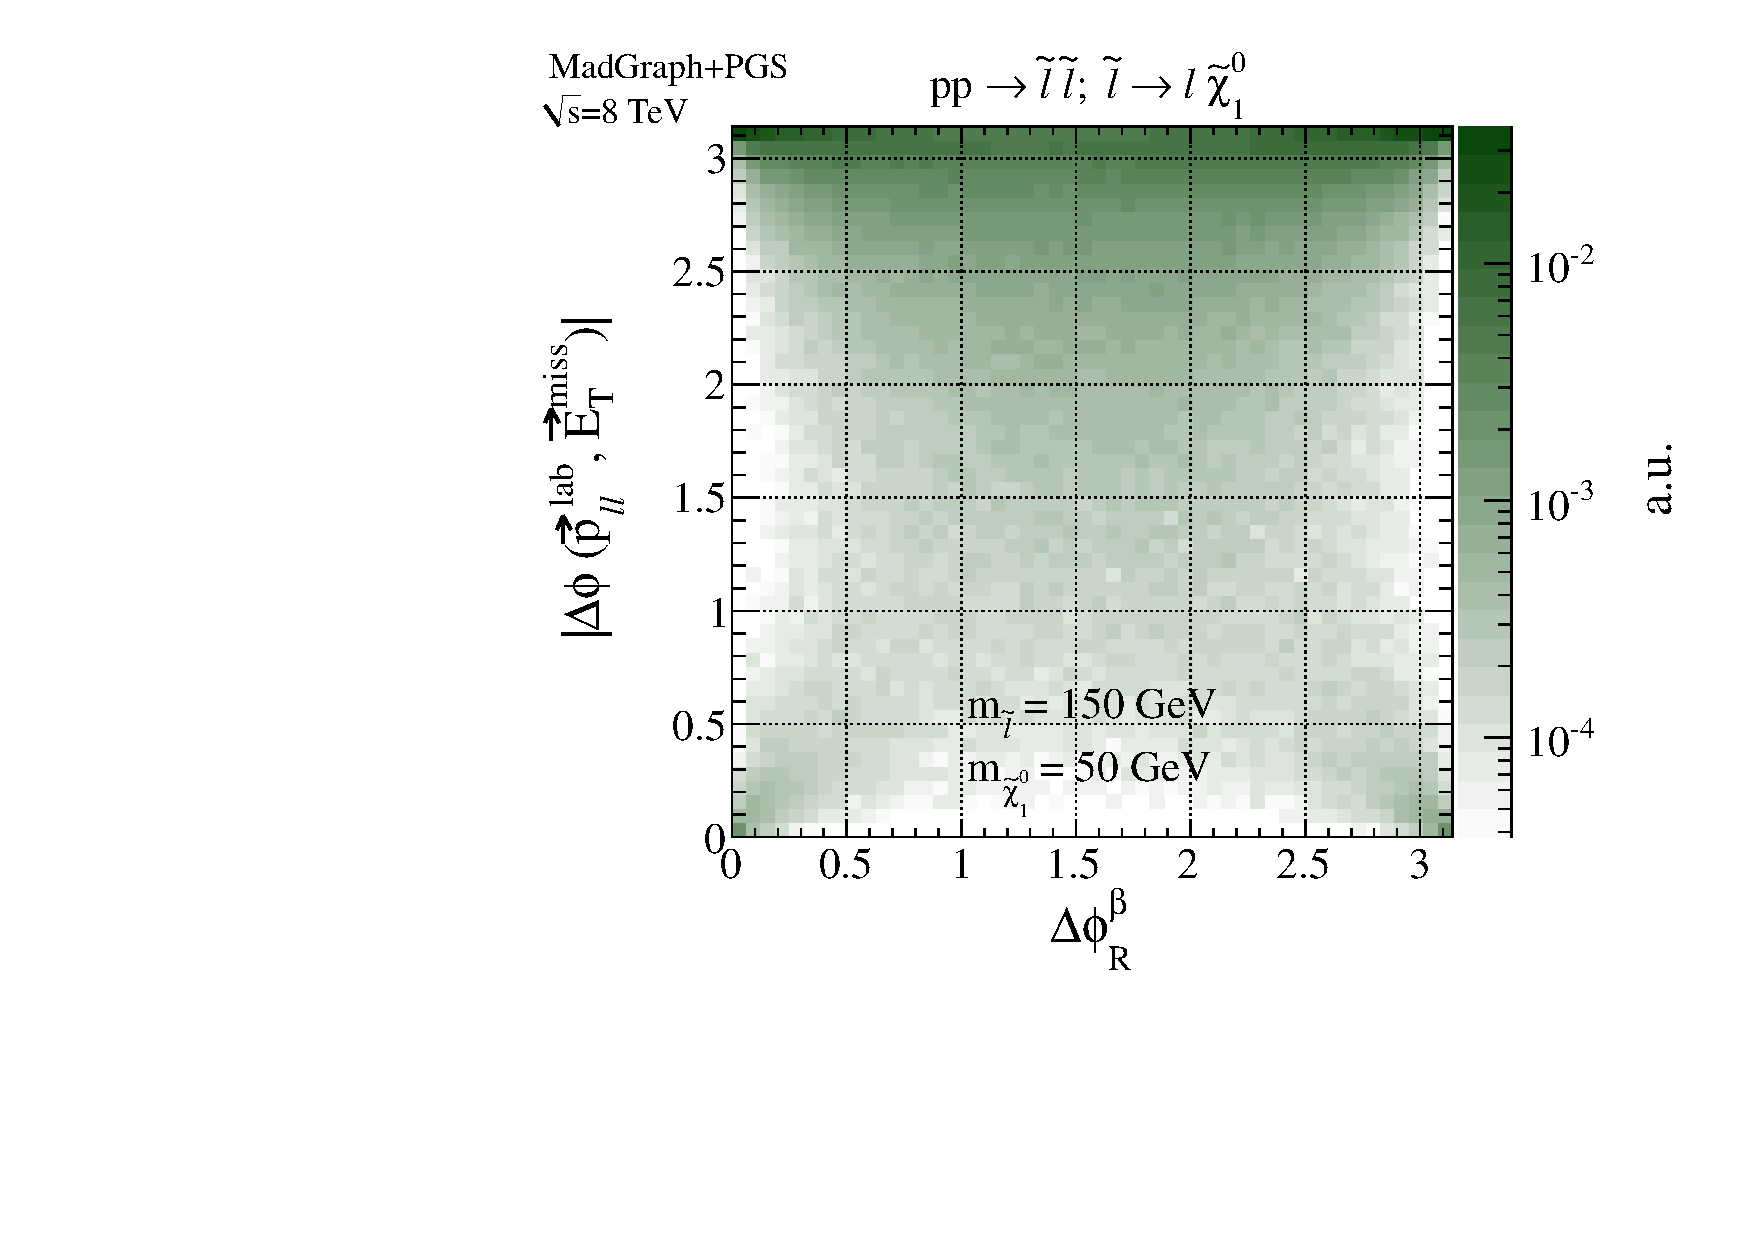
\includegraphics[width=0.3\columnwidth]{fig/sectionIII/dphi_v_dphi_slepton_150_50.pdf}
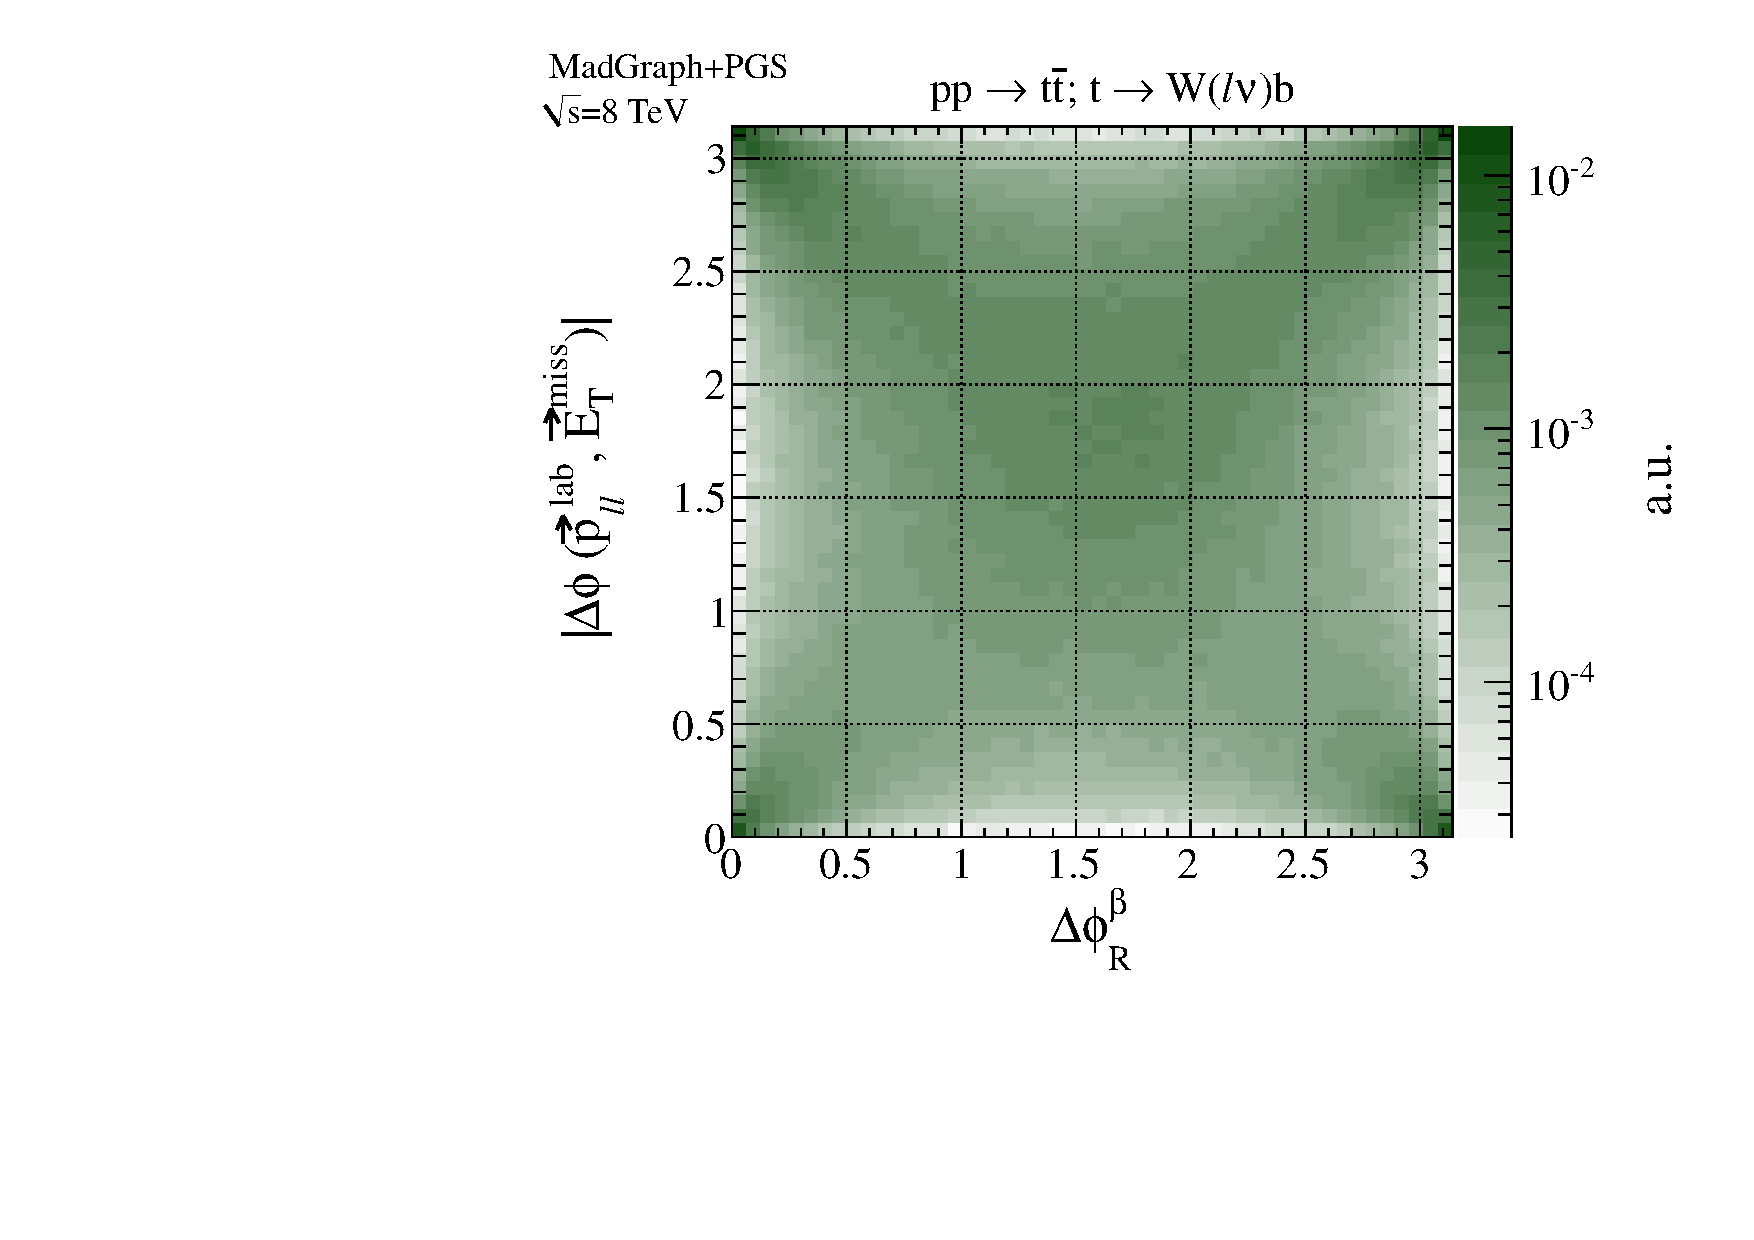
\includegraphics[width=0.3\columnwidth]{fig/sectionIII/dphi_v_dphi_ttbar.pdf}
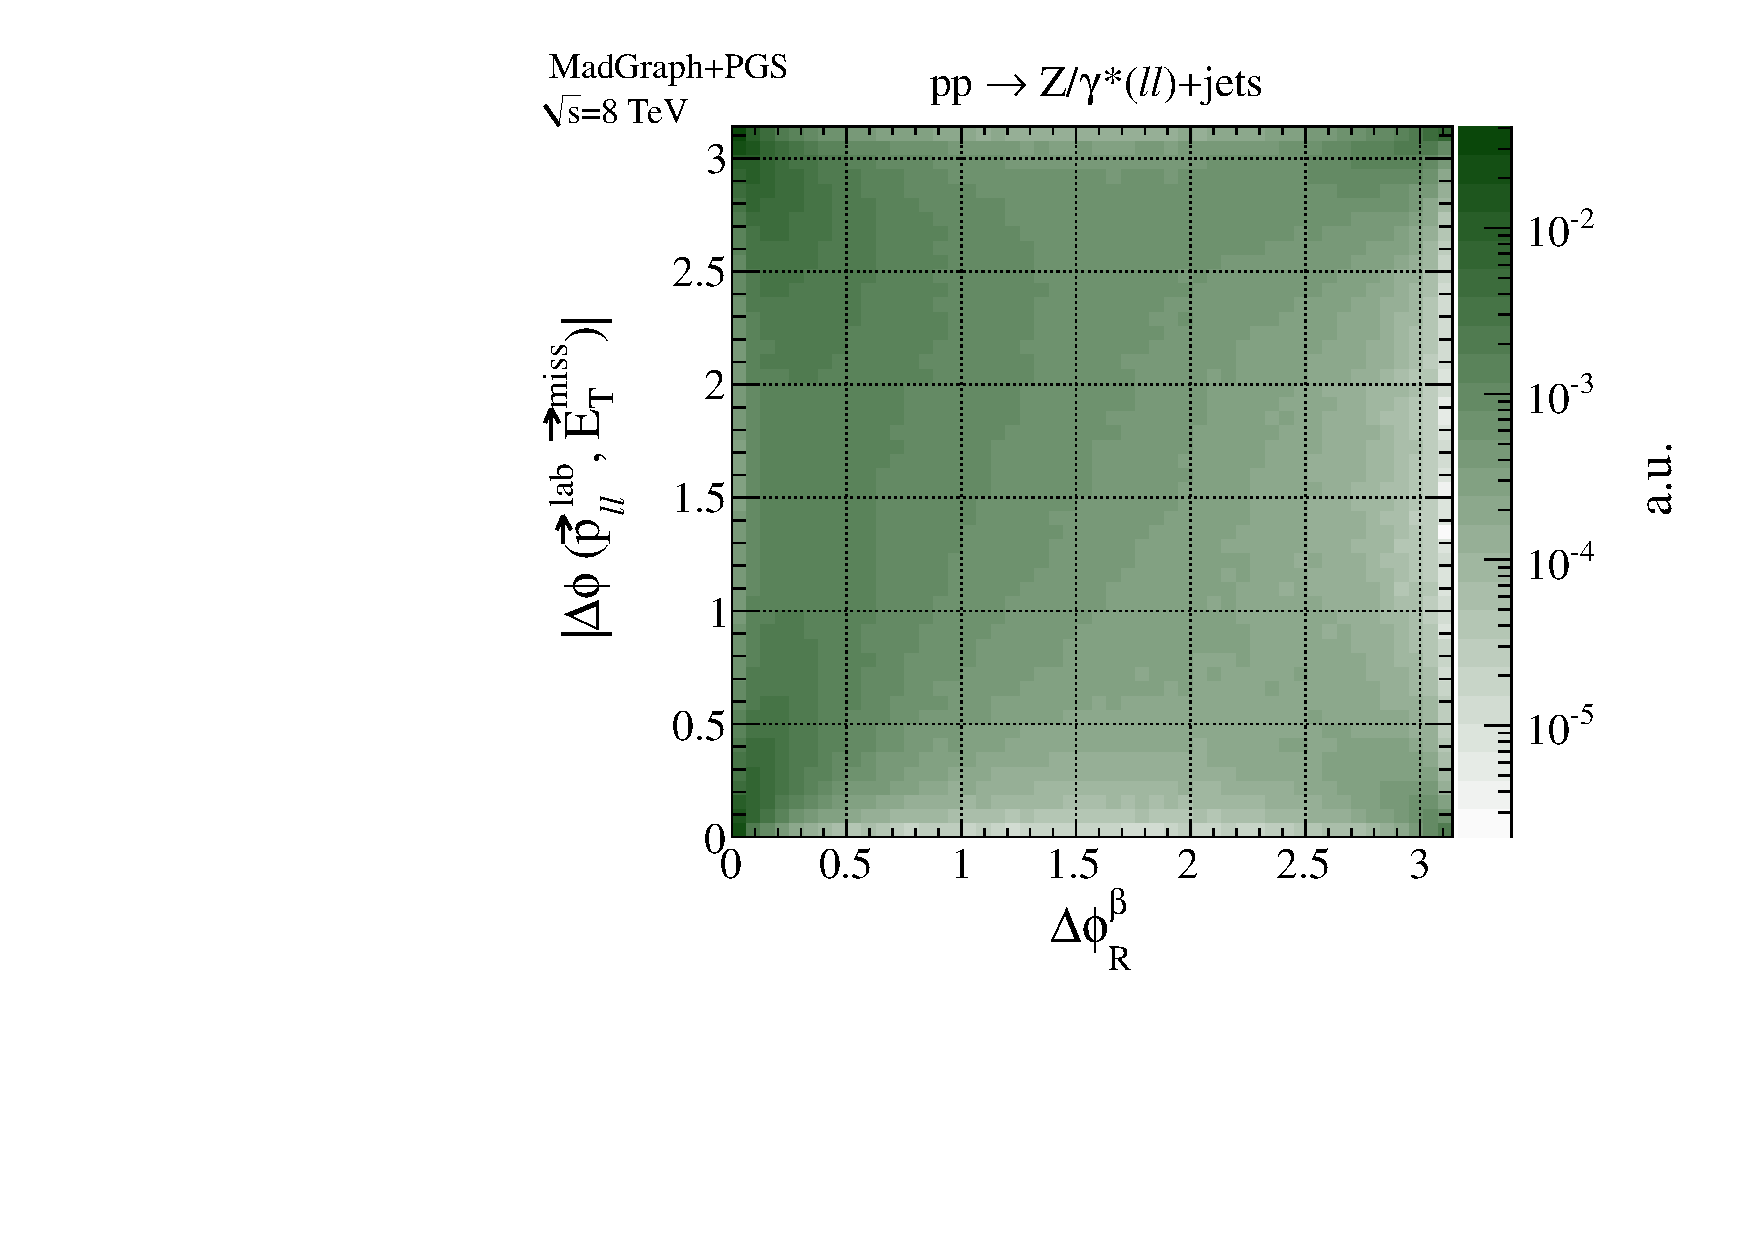
\includegraphics[width=0.3\columnwidth]{fig/sectionIII/dphi_v_dphi_DY.pdf}
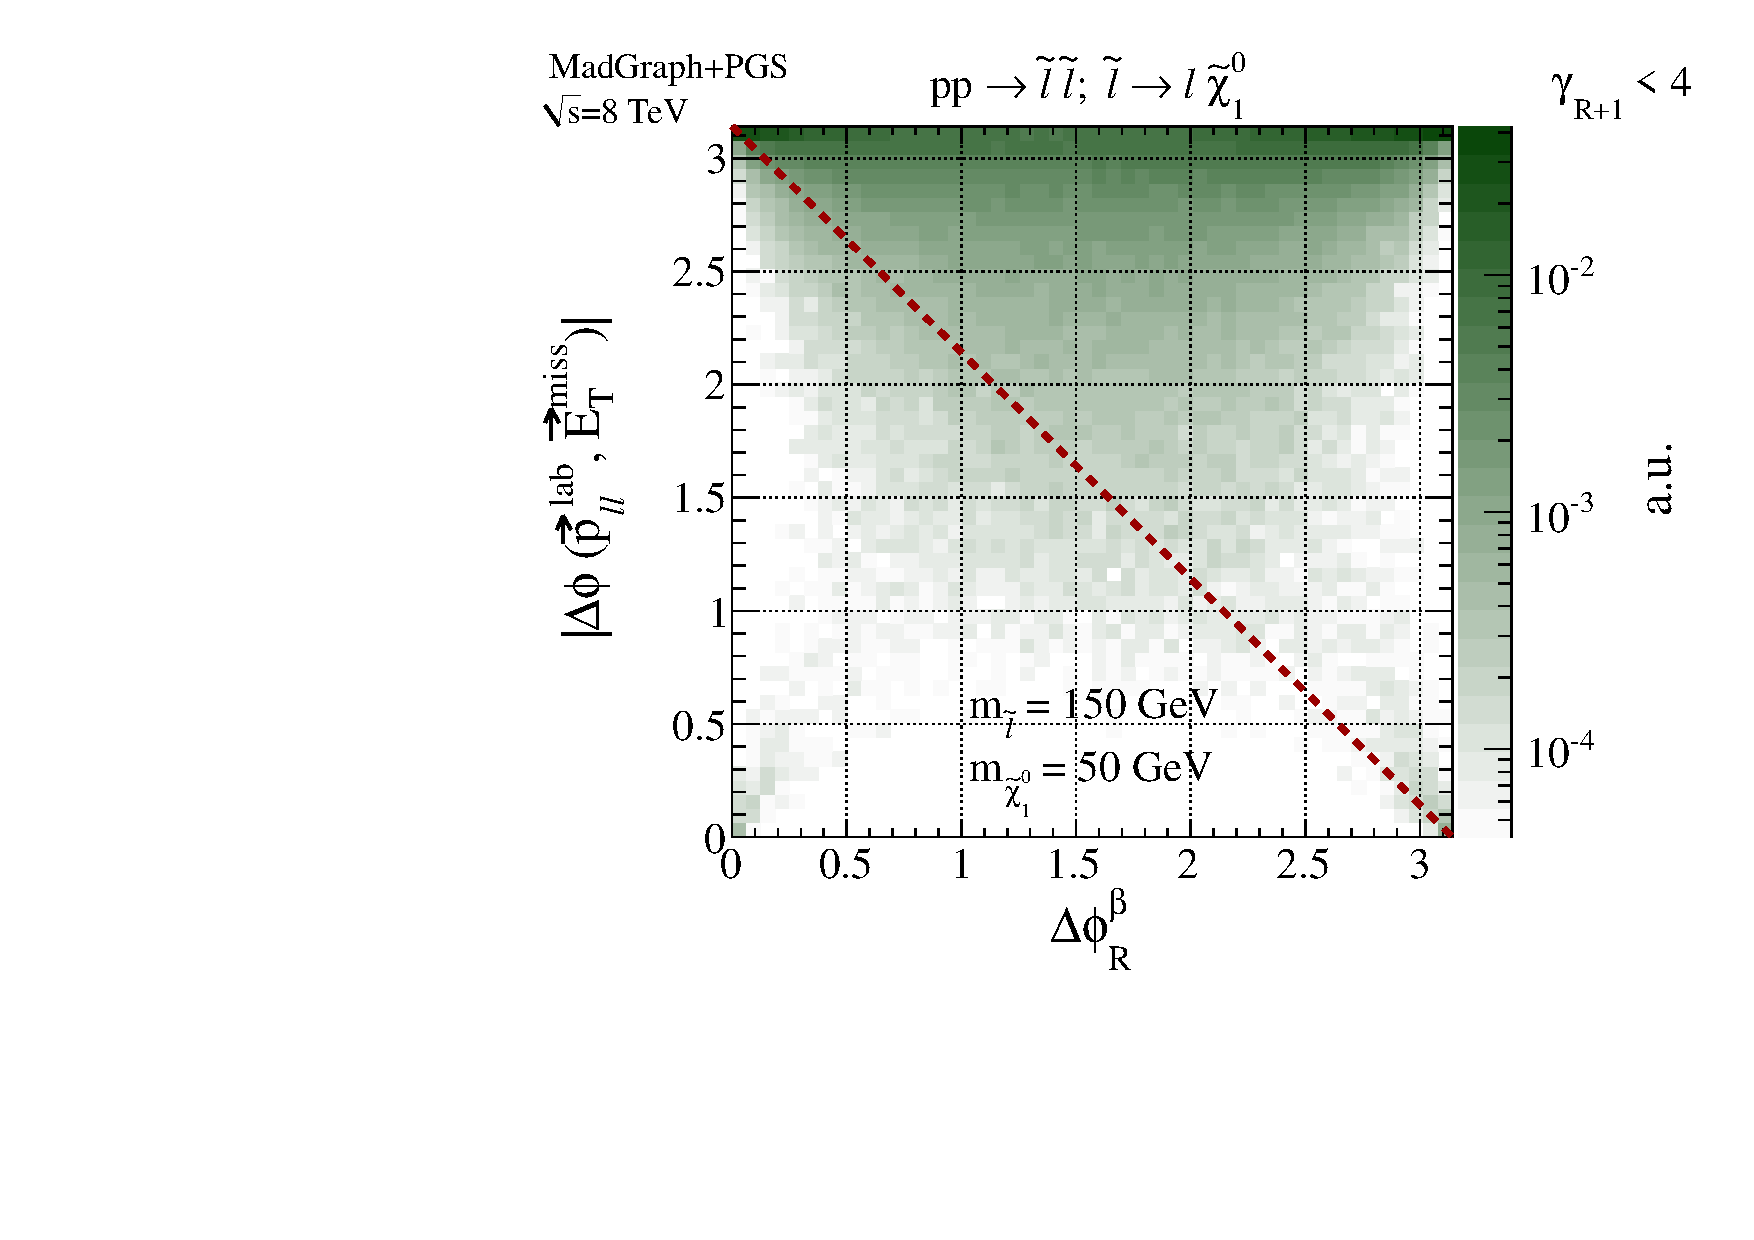
\includegraphics[width=0.3\columnwidth]{fig/sectionIII/dphi_v_dphi_slepton_150_50_gamma4.pdf}
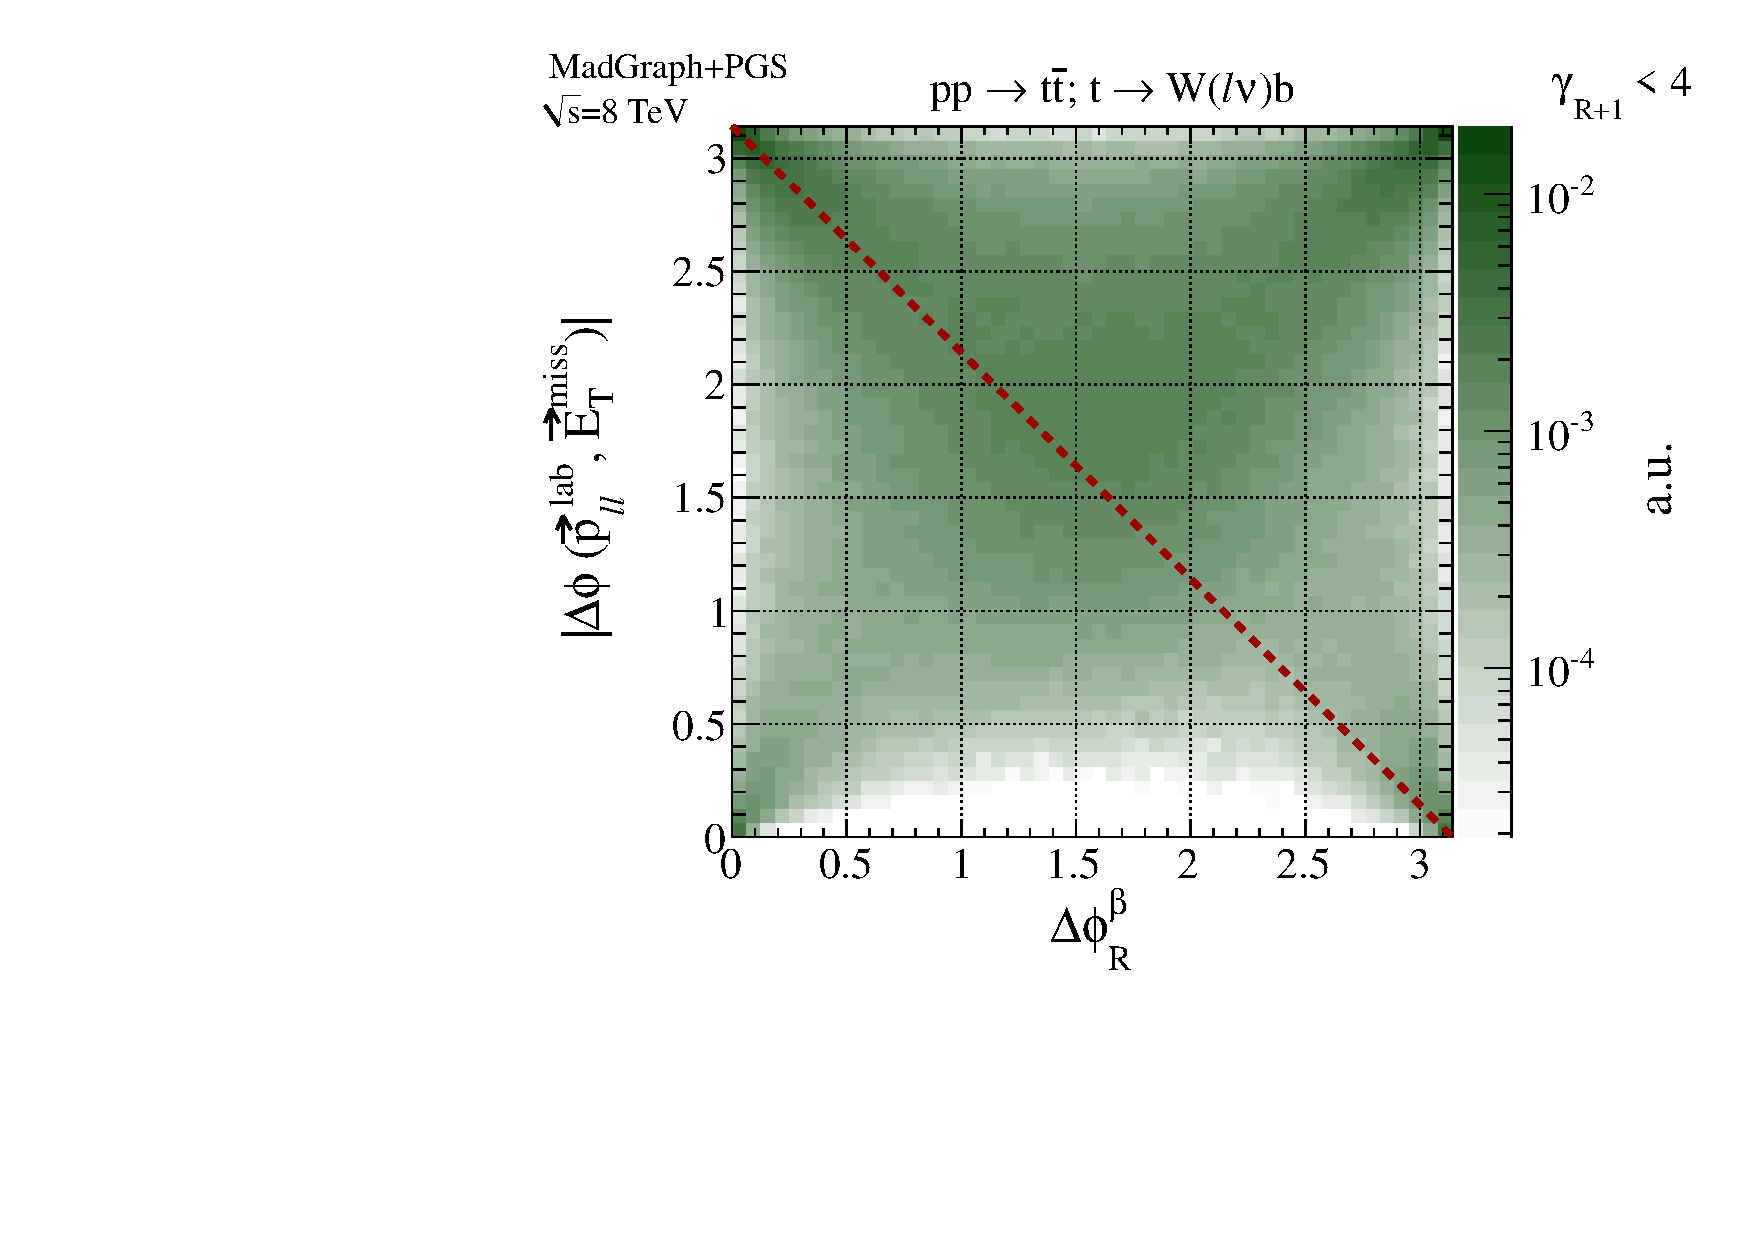
\includegraphics[width=0.3\columnwidth]{fig/sectionIII/dphi_v_dphi_ttbar_gamma4.pdf}
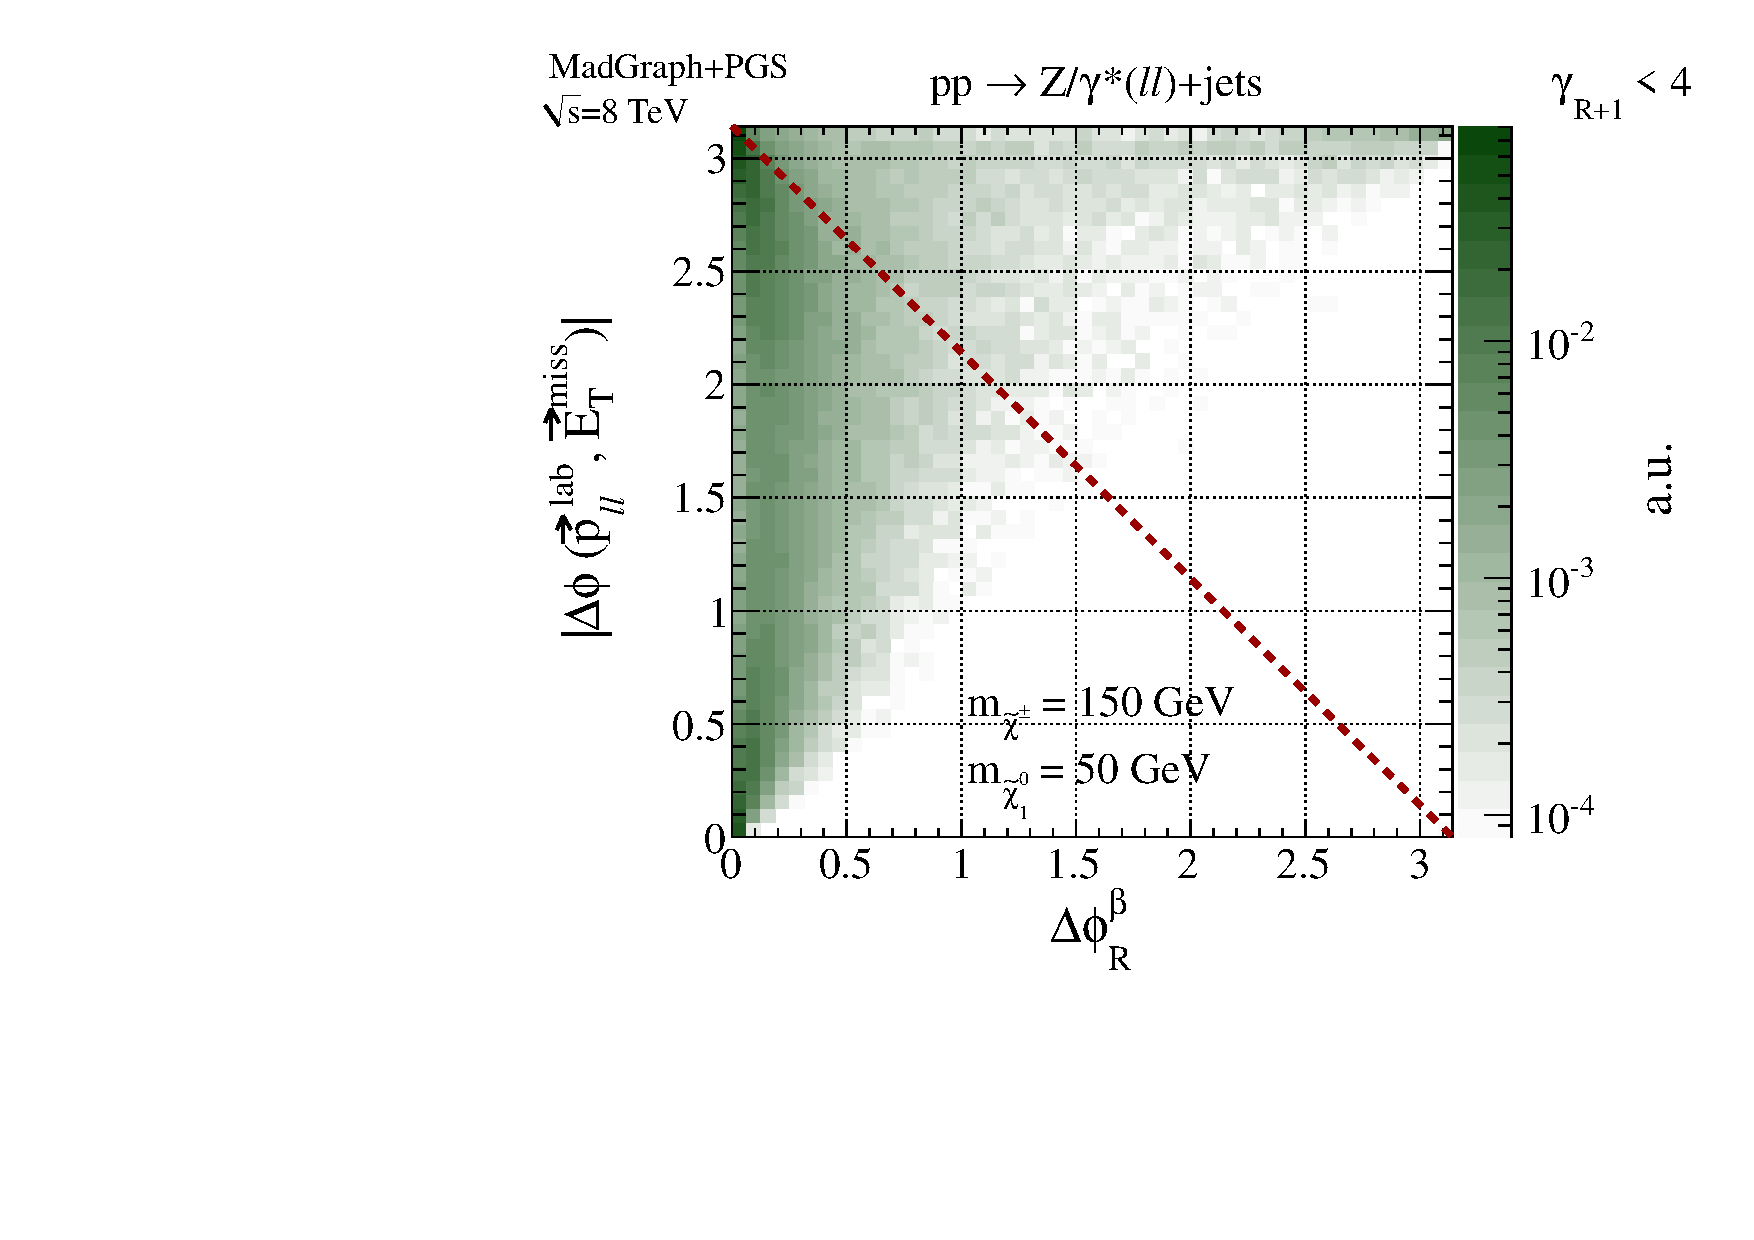
\includegraphics[width=0.3\columnwidth]{fig/sectionIII/dphi_v_dphi_DY_gamma4.pdf}
\caption{Distributions of $|\Delta\phi (\vec{p}_{\ell\ell}^{\, \text{lab}},\vec{E}_{T}^\text{miss})|$ vs. $\Delta \phi_{R}^{\beta}$ for simulated events samples. Top row: inclusive baseline event selection. Bottom row: additional $\gamma_{R+1} > 4$ requirement. Samples correspond to di-slepton production (left), di-leptonic $t\bar{t}$ (center), and $Z/\gamma^{*}$+jets. \label{fig:dphi_v_dphi}}
\end{figure}

As discussed in Section~\ref{sec:variables}, the variable $|\cos\theta_{R+1}|$ is also useful for rejecting Drell-Yan background, independently of the $\Delta\phi_{R}^{\beta} + |\Delta\phi (\vec{p}_{\ell\ell}^{\, \text{lab}},\vec{E}_{T}^\text{miss})| > \pi$ requirement. Rather than include requirements on $|\cos\theta_{R+1}|$ in the selection we will use the full distribution as a descriminating variable in an analysis described in the following section. We define the Razor event selection as: \\ \\
{\bf Razor selection:}\\
\begin{tabular}{c c}
~~~~~~~~~~~~~~~~~~~~~~~~~~~~~~~~SF Channels ($ee$,$\mu\mu$)~~~~~~~~~~~~~~~~~~~~~~~~~~~~~~~~ & OF channels ($e\mu$) \\
& \\
$\gamma_{R+1} < 10$ &  \\
$|m(\ell\ell) - m_{Z}| > 10$~GeV  &  None\\
$\Delta\phi_{R}^{\beta} + |\Delta\phi (\vec{p}_{\ell\ell}^{\, \text{lab}},\vec{E}_{T}^\text{miss})| > \pi$ & 
\end{tabular} \\

Used in conjunction with $|\cos\theta_{R+1}|$, this simple event selection sufficiently reduces the $Z/\gamma^{*}$+jets background to a manageable level, without appealing to 
$E_{T}^\text{miss}$ cuts that decrease selection efficiency for signals with lower $M_{\Delta}$. There is likely room for optimization in these cuts, but this combination is sufficient for demonstrating that gains in sensitivity are possible for more compressed spectra, as we will see in the following sections. The efficiencies and expected cross-sections of event yields with the Razor selection applied for the slepton and chargino signal models considered are summarized in Figure~\ref{fig:EFF_Razor}. Analogous values for simulated background processes are provided in Table~\ref{tab:BKG}. We observe that the efficiency for selecting low $M_{\Delta}$ events is improved over the CMS and ATLAS selections, while the number of $Z/\gamma^{*}$+jets at high $M_{\Delta}^{R}$ are reduced.

\begin{figure}[ht]
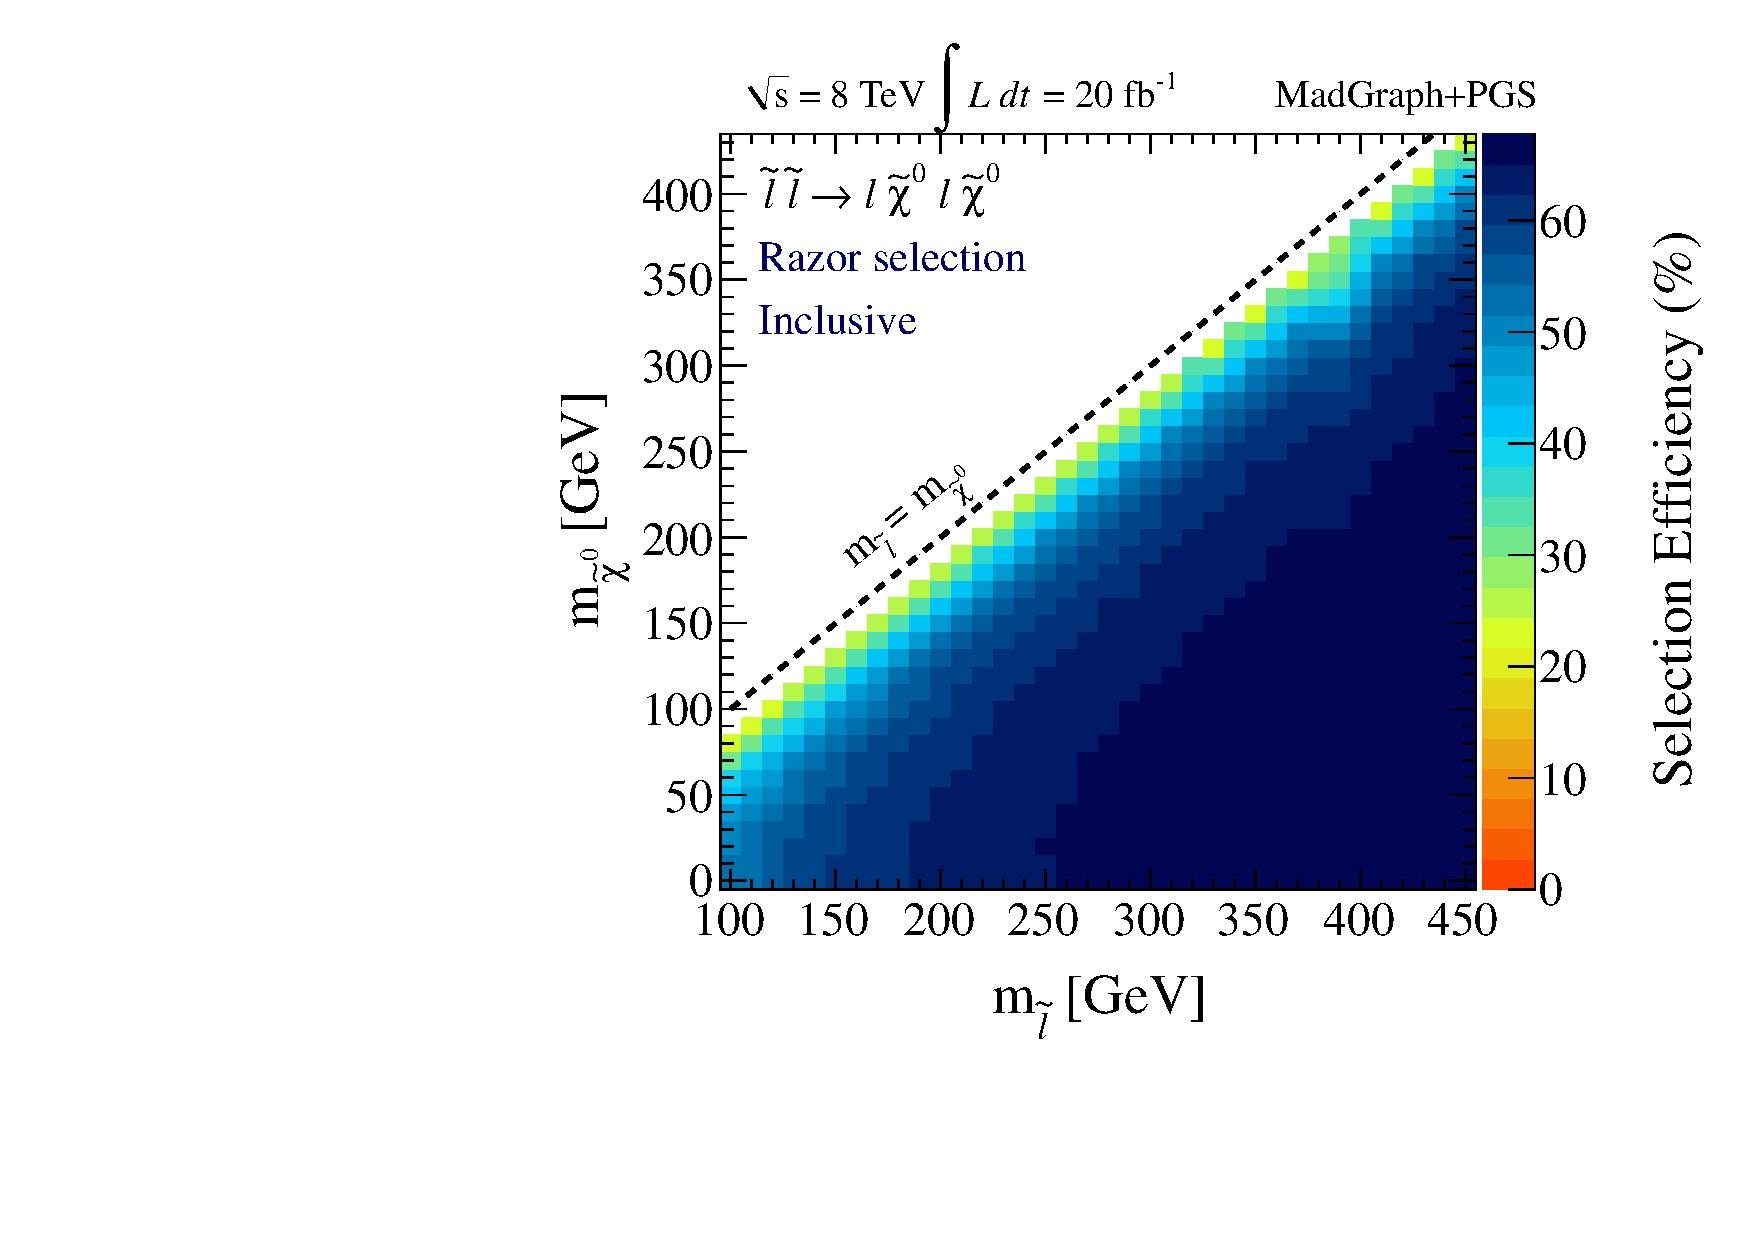
\includegraphics[width=0.3\columnwidth]{fig/sectionIII/EFF_slepton_Razor_incl.pdf}
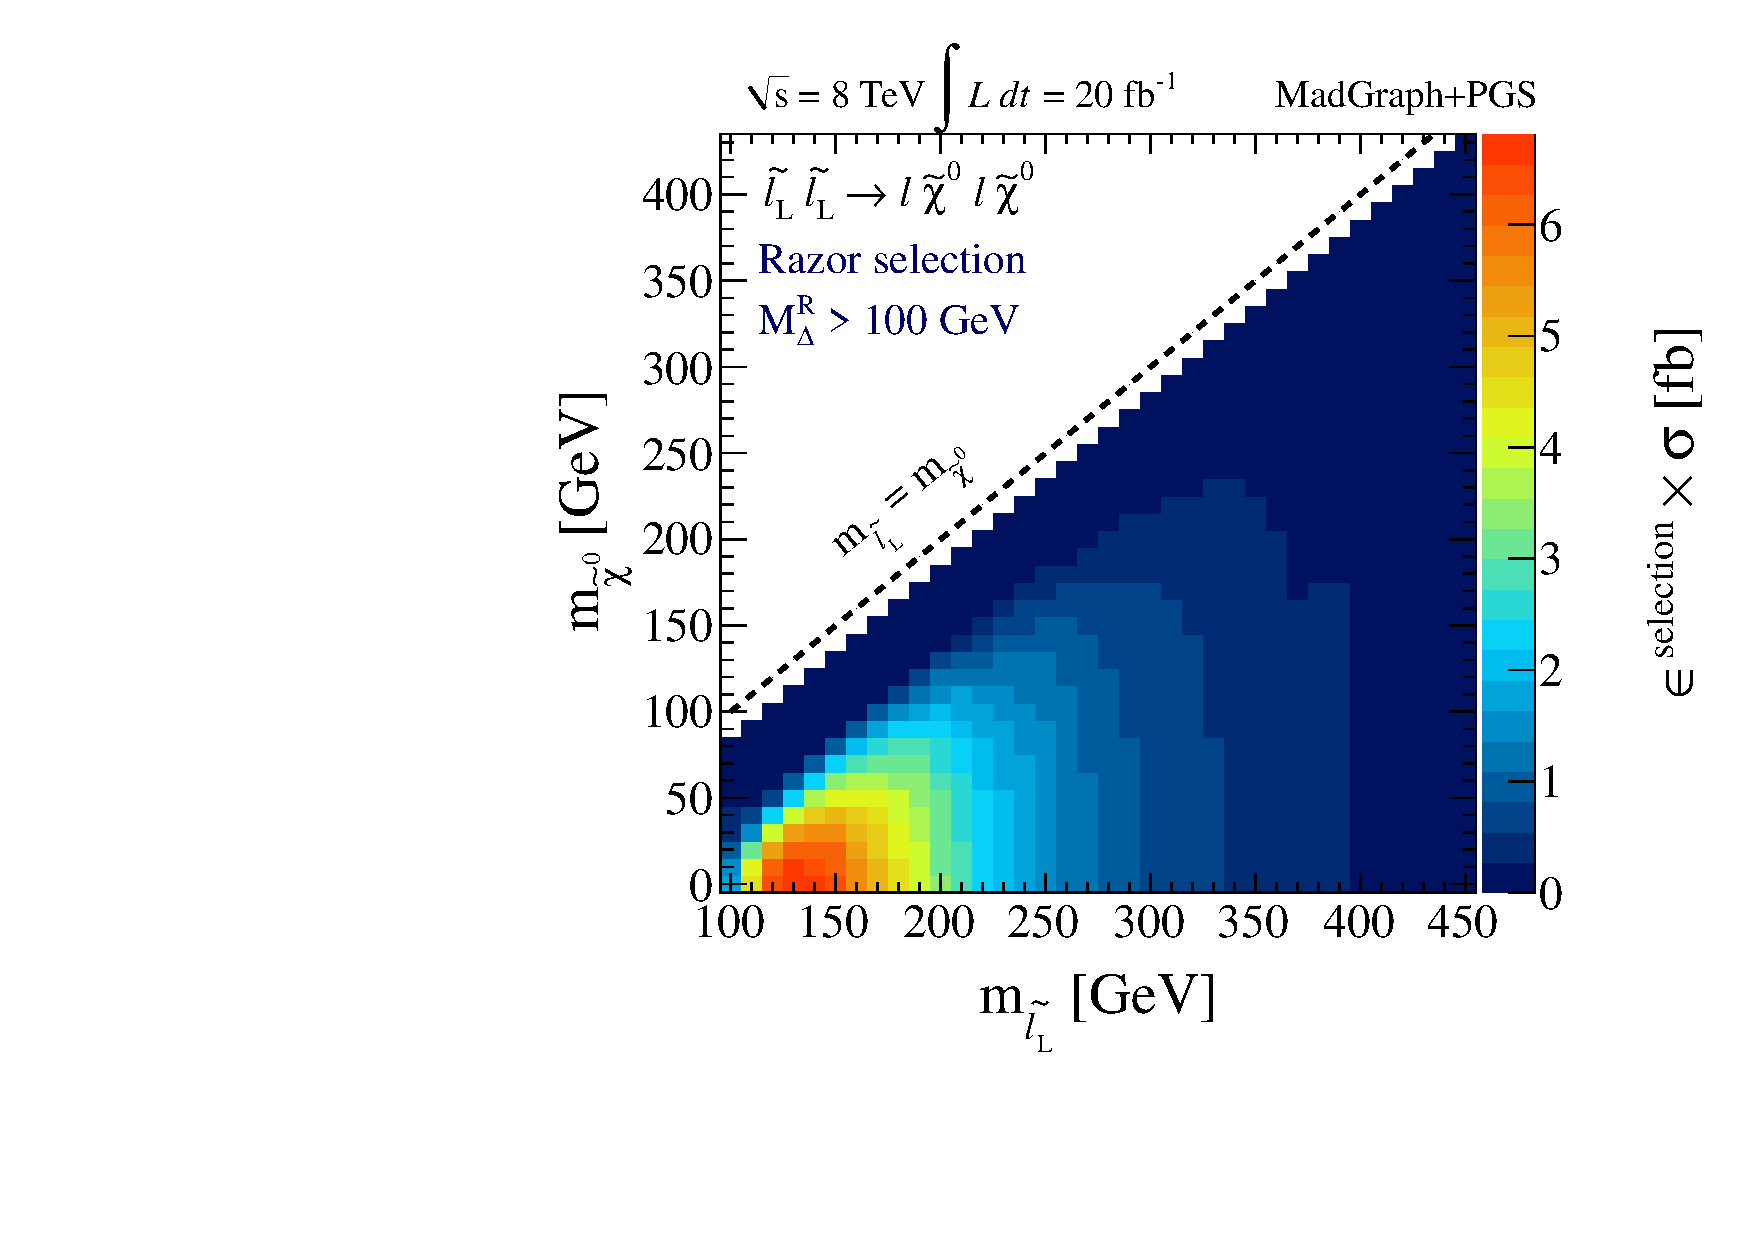
\includegraphics[width=0.3\columnwidth]{fig/sectionIII/XSEC_sleptonL_Razor_Mdelta100.pdf}\\
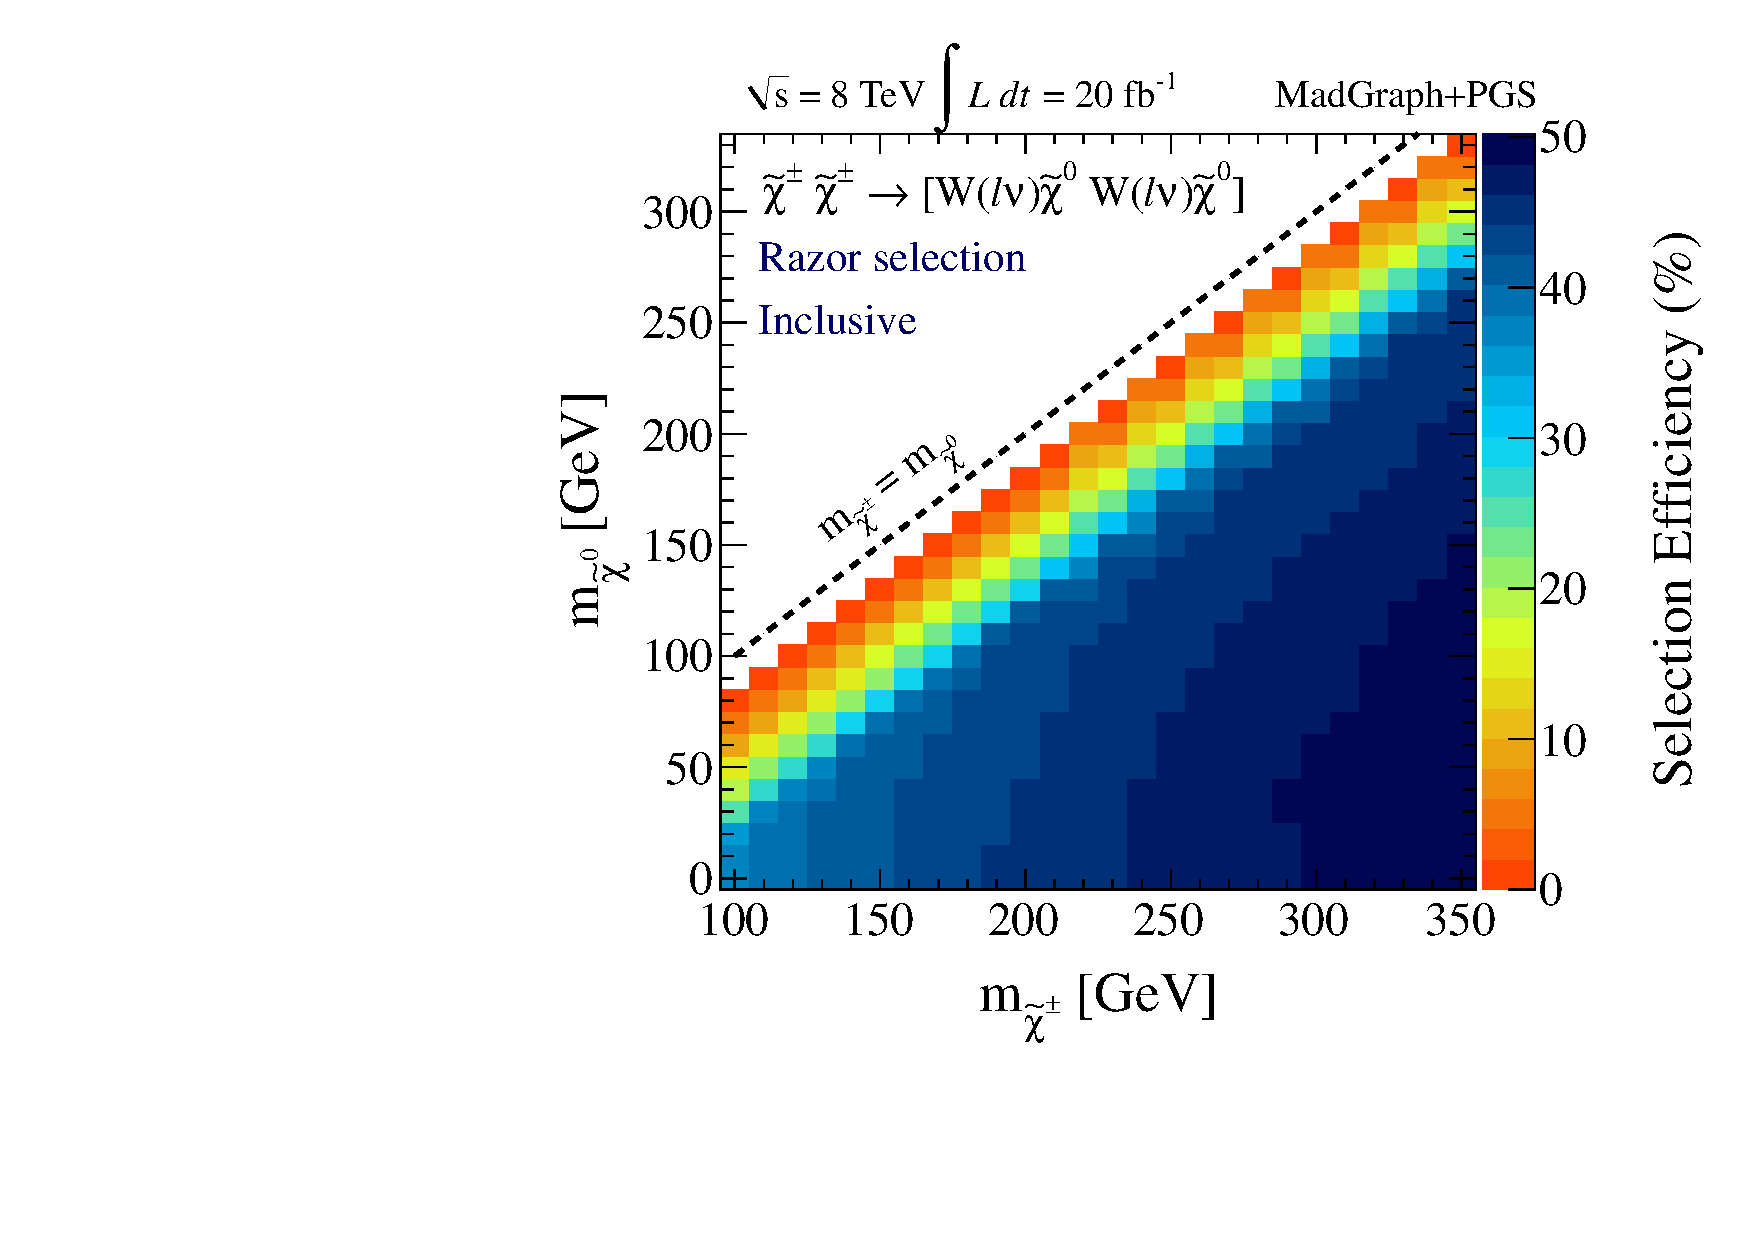
\includegraphics[width=0.3\columnwidth]{fig/sectionIII/EFF_chargino_Razor_incl.pdf}
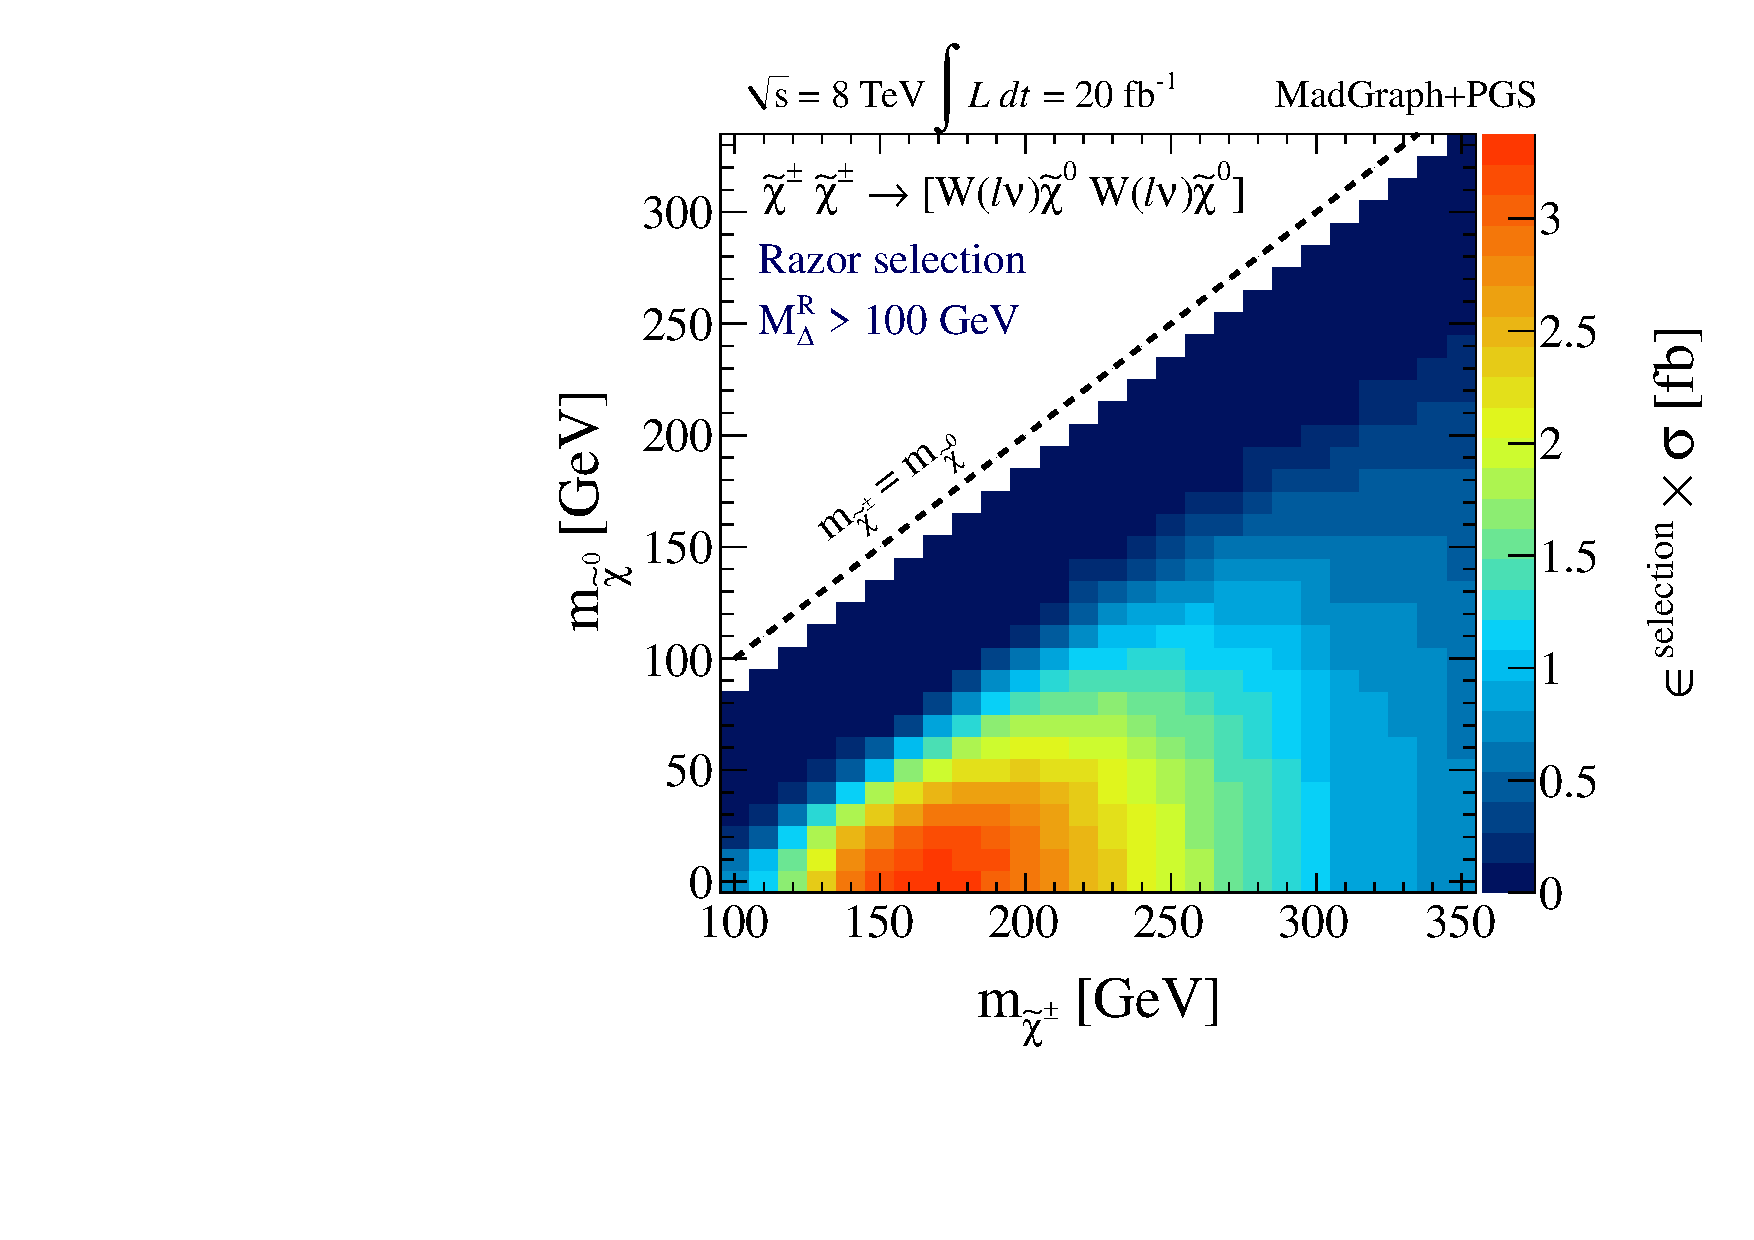
\includegraphics[width=0.3\columnwidth]{fig/sectionIII/XSEC_chargino_Razor_Mdelta100.pdf}
\caption{Selection efficiencies (left) and efficiency times cross section (right) for left-handed selectrons (upper row) and chargino (lower row) signal samples, as a function of neutralino mass for the Razor selection criteria, described in the text.  \label{fig:EFF_Razor}}
\end{figure}


\begin{table}[ht]
\begin{tabular}{|c|c|c|c|c|c|c|c|} \hline
 \multicolumn{2}{|c|}{$\sigma \times \epsilon$~[fb]}   & \multicolumn{2}{|c|}{CMS selection} & \multicolumn{2}{|c|}{ATLAS selection} & \multicolumn{2}{|c|}{Razor selection} \\ \hline
 \multicolumn{2}{|c|}{}  & \multicolumn{2}{|c|}{Inclusive ($M_{CT\perp} > 100$~GeV)} & \multicolumn{2}{|c|}{Inclusive ($M_{T2} > 100$~GeV)} &\multicolumn{2}{|c|}{Inclusive ($M_{\Delta}^{R} > 100$~GeV)} \\ \hline
Process & Jet mult. & $~~~~~ ee$+$\mu\mu ~~~~~~$ & $e\mu$  & $~~~~~ ee$+$\mu\mu ~~~~~~$ & $e\mu$ & $~~~~~ ee$+$\mu\mu ~~~~~~$ & $e\mu$ \\ \hline
                     & 0 jets            &  230 (0.067) & 280 (0.068) & 430 (0.15) & 500 (0.15) & 910 (0.55) & 1300 (0.54) \\ 
Di-Bosons  & 1 jet              &  120 (0.084) & 150 (0.085) & 120 (0.13) & 142 (0.13) & 170 (0.54) & 380 (0.86) \\ 
                     & $\ge 2$ jets &  55 (0.044) & 70 (0.061) & 37 (0.056) & 44 (0.059) & 47 (0.36) & 130 (0.78) \\ \hline         
                     & 0 jets            & 38 (0.12) & 46 (0.052) & 31 (0.14) & 34 (0.15) & 65 (0.29) & 95 (0.29) \\ 
$t\bar{t}$     & 1 jet              & 140 (0.20) & 180 (0.28) & 110 (0.29) & 120 (0.34) & 180 (0.72) & 340 (0.81) \\ 
                     & $\ge 2$ jets & 290 (0.46) & 360 (0.57) & 170 (0.50) & 200 (0.58) & 310 (1.4) & 650 (1.8) \\ \hline  
                     & 0 jets            &  70 (0.92) & 4.8 (0.037) & 160 (1.5) & 3.3 (0.046) & 1800 (1.6) & 730 ($< 0.001$)  \\ 
$Z/\gamma^*(\ell\ell)$  & 1 jet & 85 (1.3) & 37 (0.010) & 70 (1.5) & 5.2 (0.078) & 110 (0.94) & 110 ($< 0.001$)  \\ 
                     & $\ge 2$ jets & 44 (0.55) & 27 (0.001) & 13 (0.50) & 2.4 ($< 0.001$) & 46 (0.24) & 37 ($< 0.001$) \\ \hline           

%$t\bar{t}$ & $2.27 \times 10^5$ & $9.64 \times 10^{-5}$ & 21.9 & $8.91\times 10^{-5}$ & 20.2 & $2.43\times 10^{-4}$ & 55.2 \\ \hline 
%Drell-Yan & $2.56 \times 10^6$ & $4.27 \times 10^{-5}$ & 109 & $4.20\times 10^{-5}$ & 108 & $7.00 \times 10^{-6}$  & 17.9 \\ \hline 
%$W^+W^-$ & $5.88 \times 10^4$ & $1.75 \times 10^{-3}$ & 103 & $1.74 \times 10^{-3}$ & 102 & $4.35 \times 10^{-3}$ & 256 \\ \hline
\end{tabular}
\caption{Effective cross sections for di-lepton backgrounds at the LHC with $\sqrt{s} = 8$~TeV, after selection requirements (efficiency [$\epsilon$] times cross section [$\sigma$]). Cross sections are listed for each of the event selections (CMS, ATLAS and Razor) as a function of jet multiplicity and lepton flavor, with and without selection requirements on mass sensitive variables. \label{tab:BKG} }
\end{table}
%need to replace numbers with ones after cuts

